\documentclass[12pt,a4paper]{report}

% packages
\usepackage[lmargin={2.54cm},rmargin={2.54cm},tmargin={2.54cm},bmargin={2.54cm}]{geometry} % 1" margins
\usepackage[english]{babel}
\usepackage{amssymb}
\usepackage{graphicx}
\usepackage{floatrow} % for centering all figures automatically
\usepackage{tikz} % for positioning the logo
\floatsetup[table]{capposition=top} % for captions above tables
\usepackage[latin1]{inputenc}
\usepackage[bottom]{footmisc} % fix for figures under footnotes
\usepackage[backend=bibtex,style=authoryear,citestyle=authoryear]{biblatex} % for references with footnotes
\usepackage[titletoc]{appendix} % for inclusion of references in toc
\usepackage{setspace} % for spacing
\usepackage{mathtools}   % loads �amsmath�
\usepackage{amssymb} % for mathematical letters like real numbers space


\bibliography{references}

% packages only for demonstration/testing
\usepackage[textsize=tiny]{todonotes} % for todo notes
\setlength{\marginparwidth}{2.2cm} % for todo width
\usepackage{lipsum} % for lorem ipsum

\usepackage[nonumberlist,acronyms]{glossaries} % for lsit of abbreviations and list of symbols
\newglossary{symbols}{sym}{sbl}{List of Symbols}

\makenoidxglossaries

%=====================ACRONYMS=====================%
\newacronym{SMPC}{SMPC}{secure multi-party computation}
\newacronym{LAN}{LAN}{local area network}
\newacronym{MANET}{MANET}{mobile ad hoc networks}
\newacronym{SPAN}{SPAN}{smart phone ad hoc network}
\newacronym{IoT}{IoT}{Internet of Things}
\newacronym{NDK}{NDK}{Native Development Kit}
%=====================SYMBOLS=====================%
\newglossaryentry{doubleR}{	type=symbols,sort={real set}, name={\ensuremath{\mathbb{R}}} , description={set of real numbers} }


%\documentclass[12pt,a4paper]{report}
\usepackage{graphicx}
\usepackage{tikz} % for positioning the logo
\usepackage[latin1]{inputenc}

\begin{document}
	\begin{titlepage}
	\begin{tikzpicture}[remember picture,overlay]
	\node[anchor=north east,inner sep=10pt] at (current page.north east){\includegraphics[width=1.41cm,keepaspectratio]{figures/FH-logo.png}};
	\end{tikzpicture}
	\vspace{1cm}
	\centering
	{\LARGE Fachhochschule Aachen \par}
	\vspace{0.3cm}
	{\Large Campus J\"ulich \par}
	\vspace{1cm}
	{\Large Fachbereich: Medizintechnik und Technomathematik\par}
	\vspace{0.3cm}
	{\Large Studiengang: Technomathematik\par}
	\vspace{1.5cm}
	
	{\huge Secure Multi-Party Computation for Decentralized Distributed Systems\par}
	\vspace{2cm}
	{\Large Masterarbeit von Frederic Klein\par}
	\vfill
	{\large Diese Arbeit wurde betreut von:\par
	1. Pr\"ufer: Prof. Dr. rer. nat. Alexander \textsc{Vo}\ss{}\par
	2. Pr\"ufer: Dr. Stephan \textsc{Jonas}}

	\vfill
	
	% Bottom of the page
	{\large Aachen, Oktober, 2016 \par}
\end{titlepage}
\end{document}

\begin{document}

\newgeometry{left=3cm}
	\begin{titlepage}
	\begin{tikzpicture}[remember picture,overlay]
	\node[anchor=north east,inner sep=10pt] at (current page.north east){\includegraphics[width=1.41cm,keepaspectratio]{figures/FH-logo.png}};
	\end{tikzpicture}
	\vspace{1cm}
	\centering
	{\LARGE Fachhochschule Aachen \par}
	\vspace{0.3cm}
	{\Large Campus J\"ulich \par}
	\vspace{1cm}
	{\Large Fachbereich: Medizintechnik und Technomathematik\par}
	\vspace{0.3cm}
	{\Large Studiengang: Technomathematik\par}
	\vspace{1.5cm}
	
	{\huge Secure Multi-Party Computation for Decentralized Distributed Systems\par}
	\vspace{2cm}
	{\Large Masterarbeit von Frederic Klein\par}
	\vfill
	{\large Diese Arbeit wurde betreut von:\par
	1. Pr\"ufer: Prof. Dr. rer. nat. Alexander \textsc{Vo}\ss{}\par
	2. Pr\"ufer: Dr. Stephan \textsc{Jonas}}

	\vfill
	
	% Bottom of the page
	{\large Aachen, Oktober, 2016 \par}
\end{titlepage}
\restoregeometry

\pagenumbering{roman}

\clearpage
\vspace*{\fill}
\begin{center}
	\begin{minipage}{.8\textwidth}
		\thispagestyle{empty} % no pagenumber on affidavit
		Diese Arbeit ist von mir selbst\"andig angefertigt und verfasst. Es sind keine anderen als die angegebenen Quellen und Hilfsmittel benutzt worden.\par
		\vspace{1cm}
		Frederic Klein \dotfill \par
		Unterschrift
	\end{minipage}
\end{center}
\vfill % equivalent to \vspace{\fill}
\clearpage

\spacing{1.5} % line spacing

\begin{abstract}
	\thispagestyle{plain}
	\setcounter{page}{1}
	In recent years gamification has become a part in many areas of our daily routine. In regard to our personal life, companies like Amazon or Runtastic can base their gamification approach on publicly sharing personal achievements and statistics to improve user commitment. In contrast, gamification concerning our work life has to satisfy much higher privacy demands. Since comparison is a key component for gamification, privacy protecting computations of system wide statistical values (for example minimum and maximum) are needed. The solution comes in the form of \gls{SMPC}, a subfield of cryptography. Existing frameworks for \gls{SMPC} utilize the Internet Protocol, though access to the Internet or even a \gls{LAN} cannot be provided in all environments. Facilities with sensible measuring systems, e.g. medical devices in hospitals, often avoid Wi-Fi to reduce the risk of electromagnetic interference.
	To be able to utilize \gls{SMPC} in environments with Wi-Fi restrictions, this thesis studies the characteristics of \gls{MANET} and proposes the design of a \gls{SMPC} framework for \gls{MANET}, especially based on Bluetooth technology, and the implementation as a C library.
	
	Since \glspl{MANET} have a \todo*{bad word high acceptable here?} high probability for network partition, a centralized architecture for the computation and data preservation is unfavorable. Therefor a blockchain based distributed database is implemented in the framework. Typical problems of distributed systems are addressed with the implementation of algorithms for clock synchronization and coordinator election as well as protocols for the detection of computation partners and data distribution. Since the framework aims to provide distributed computations of comparable values, protocols for secure addition and secure comparison are implemented, enabling the computation of minimum, maximum and average.
	
	Devices of diverse computational power will be used to verify the applicability for wearables and \gls{IoT} grade devices. Also field-tests with a \gls{SPAN}(20-50 nodes) will be conducted to evaluated real life use cases. In contrast, the security of the framework and attack scenarios will be discussed. In summary, this thesis proposes a framework for \gls{SMPC} for decentralized, distributed systems.
\end{abstract}

\glsunsetall

\tableofcontents
\setcounter{page}{2}
\listoffigures
{\let\clearpage\relax \listoftables}

\glsresetall

\printnoidxglossary[type=\acronymtype,title={List of Acronyms}]

{\let\clearpage\relax \printnoidxglossary[type=symbols,sort=letter]}


\chapter{Introduction} \label{Introduction}
\todo*{5-10\%, including motivation, general audience}

\pagenumbering{arabic}
%In the last couple of years gamification has found it's way into many areas of our daily life. In regard to our personal life, companies like Amazon or Runtastic can base their gamification approach on publicly sharing personal achievements and statistics to improve user commitment. In contrast, gamification concerning our work life can have much higher privacy demands. Since comparison is a key component for the gamification approach, privacy protecting computations of system wide statistical values (for example minimum and maximum) are needed. The solution comes in the form of \gls{SMPC}, a subfield of cryptography.

%Existing frameworks for \gls{SMPC} utilize the Internet protocol, though access to the Internet or even a \gls{LAN} cannot be provided in all environments. Especially many hospitals tend to avoid Wi-Fi to reduce the risk of electromagnetic interference with medical devices.

%To be able to utilize \gls{SMPC} in environments with Wi-Fi restrictions, this thesis studies the characteristics of mesh-networks and proposes describes the design of a \gls{SMPC} framework for mesh-networks.

%Context

\todo*{mention \gls{IoT} problems ( \gls{DDoS} and botnets), to emphasis usefulness of connected but not online}

%Restatement of the problem

%Restatement of the response

%Roadmap

\section{Case Study: "The Hygiene Games"} \label{Case Study: "The Hygiene Games"}

\paragraph{Gamification}

\paragraph{Wireless Networks in Hospitals}

\FloatBarrier



\chapter{Background} \label{Background}

\todo*{10-15\%; thorough review of the state of the art; informed audience}


In this chapter a general understanding of \gls{SMPC} and the key features of \glspl{MANET} is established.  

First the idea for \gls{SMPC} is introduced in \ref{Secure Multi-Party Computation} \nameref{Secure Multi-Party Computation}. Since secret sharing is used for the development of \gls{SMPC} protocols, Shamir's secret sharing scheme is presented in \ref{Secret Sharing} \nameref{Secret Sharing}.
Protocols for secure addition and secure comparison with passive security are introduced in \ref{Secure Addition Protocol} and \ref{Secure Comparison Protocol} and existing frameworks for \gls{SMPC} are briefly discussed in \ref{Existing Frameworks}.

To be able to define requirements for the new framework (see \ref{Requirements}), the key features of \glspl{MANET} are identified in \fullref{Mobile Ad Hoc Networks}, with a focus on the wireless technology standards Bluetooth and Wi-Fi and the differences to similar network types like mesh networks.

%Since the \gls{SMPC} protocols expect a secure communication channel, while a pairing-less connection doesn't provide security by default, public key cryptography is needed (see \ref{Securing the Communication Channel}). 
%The key generation, as well as Shamir's secret sharing scheme, requires random numbers. Computer systems can generate pseudo-random numbers and the randomness of such an \gls{PRNG} is discussed in\fullref{Communication Layer}.

\section{Secure Multi-Party Computation} \label{Secure Multi-Party Computation}

\todo*{general idea}
\gls{SMPC} is a subfield of cryptography. The target of \gls{SMPC} is to run computations over inputs from multiple parties while keeping these inputs secret. In 1982 Yao described the problem of two millionaires trying to find out, which one is wealthier, without giving each other information about their actual capital \autocite{Yao1982}. Yaos solution for this \gls{2PC} is considered to be the basis for general \gls{SMPC} protocols.
\textcite{Cramer2015} describe for example benchmark analysis as a use-cases for \gls{SMPC}: companies want to know how well they are doing in their business area compared to other companies, while they do not want to share their current business numbers with competitors. Using a protocol for secure comparison (as described in \fullref{Secure Comparison Protocol}) the companies can calculate the best performer without leaking business information. 
\textcite{Clifton2002} describe privacy preserving data mining as another use-case: data mining on patient data can for example be used to indicate disease outbreaks but there is of course a privacy concern. Using \gls{SMPC} algorithms, statistics can be computed while keeping the personal patient data private.

For \gls{SMPC} two types of adversaries have to be considered: semi-honest and malicious adversaries.
Semi-honest adversaries "follow the protocol specification, yet may attempt to learn additional information by analyzing the transcript of messages received during the execution" \autocite{Aumann2007}. Malicious adversaries "are not bound in any way to following the instructions of the specified protocol" \autocite{Aumann2007}.
\gls{SMPC} protocols that can tolerate semi-honest parties (up to a specific threshold) provide semi-honest or passive security. \gls{SMPC} protocols that are secure against malicious adversaries achieve malicious or active security.
\textcite[p. 82]{Cramer2015} also differentiate between unconditional or perfect security and computational security: if security can be proven for an adversary with unlimited computation power a protocol has unconditional security. In contrast, computational security can only be proven for a polytime adversary.

Since the target group for the protocols used in this thesis are gamification systems potential adversaries are likely of the semi-honest type. Gamification system are usually based on intrinsic motivation. Especially in the context of workplace related gamification without public recognition, there is nothing to be gained from trying to corrupt the system, only the significance of the computation results is reduced.

Honest, but curious parties are more likely, but providing the majority of semi-honest parties (which is the requirement for gaining additional information from combined shares, see \ref{Secret Sharing}), requires considerable efforts. Even if single scores are revealed, their isolated information content is almost valueless for the adversaries and targeting specific nodes over a longer amount of time adds additional complexity because of the spatial degree of freedom of the nodes (compare \ref{Mobile Ad Hoc Networks}).
Therefor, in context of gamification systems, this thesis focuses on practical \gls{SMPC} protocols for passive security based on secret sharing.

\subsection{Secret Sharing}	\label{Secret Sharing}

\textcite[p. 32]{Cramer2015} describe secret sharing schemes as the main tool to build a \gls{SMPC} protocol with passive security. In 1979 Adi Shamir described a $(k, n)$ threshold scheme for sharing secret data $D$: "Our goal is to divide $D$ into $n$ pieces $D_i$, ..., $D_n$ in such a way that:
(1) knowledge of any k or more $D_i$ pieces makes $D$ easily computable; (2) knowledge of any $k-1$ or fewer $D_i$ pieces leaves $D$ completely undetermined (in the sense that all its possible values are equally likely)" \autocite{Shamir1979}.
Shamir's secret sharing scheme is based on polynomials of degree $k-1$ with $a_0=D$ (compare \ref{eq:polynomial}). 
\begin{equation}
\label{eq:polynomial}
q(x)=\underbrace{D}_{a_0} + a_1 \cdot x + ... + a_{k-1} \cdot x^{k-1}
\end{equation}

To divide $D$ into $n$ pieces the polynomial is evaluated: $D_i=q(i),\ i=1,...,n$. For cryptographic protocols it is not practical to work with real arithmetic, instead a finite field is used: \textcite{Shamir1979} specifies that modular instead of real arithmetic is used. A prime $p$ with $p>D$, $p>n$ is selected and used to define the set $[0, p)$. "The coefficients $a_1, ..., a_{k-1}$ in $q(x)$ are randomly chosen	from a uniform distribution over the integers in $[0, p)$, and the values $D_1, ..., D_n$ are computed modulo $p$" \autocite[p. 613]{Shamir1979} (compare \ref{eq:polynomial modular}).
\begin{equation}
\label{eq:polynomial modular}
q(x) = D + a_1 \cdot x + ... + a_{k-1} \cdot x^{k-1} \mod p \qquad D,\ a_i \in [0,p)\ , \quad p \in \gls{doubleP}
\end{equation}
\textcite[p. 7]{Cramer2015} declare the set restricted by $p$ as $\mathbb{Z}_p = \{0, 1, ..., p-1\}$. They also use the notion \textit{secret S} for the data to be shared and \textit{shares $s_i$} for the computed pieces of the secret.

\todo*{describe number off messages, usage of threshold as trade-off between security and performance -> START}

\todo*{describe number off messages, usage of threshold as trade-off between security and performance -> END}

The reconstruction of a secret $S$ can be done using Lagrange interpolation (compare \ref{eq:SSS lagrange interpolation}).
\begin{equation}
\label{eq:SSS lagrange interpolation}
S = \sum_i s_i \prod_{i \neq j} \frac{-x_j}{x_i-x_j} \mod p
\end{equation}
$k$ shares $s_i$ are needed to reconstruct $S$, so only the associated values for $i$ are used in the Lagrange interpolation.

\subsubsection*{Example Computation} \label{Example Computation}

Consider the following task: a secret $S=8$ is supposed to be shared among $n=4$ parties $P_i,\quad i=1,...,4$. The threshold for the number of needed shares for the reconstruction of the secret shall be $k=3$ (public).

First a prime $p$ has to be chosen, which has to be larger than the secret ($p>S$) and the number of parties ($p>n$): $p=17$ (public information)

Since $k=3$, the polynomial has a degree of $k-1=2$ (compare \ref{eq:SSS example polynomial}).
\begin{equation}
\label{eq:SSS example polynomial}
f(x) = S + a_1 \cdot x + a_2 \cdot x^2 \mod p
\end{equation}

The coefficients are selected randomly uniformly out of $\mathbb{Z}_p=\{0,1,...,p-1\}=\{0,1,...,16\}$: $a_1=13$ and $a_2=4$ and the shares $s_i$ are computed (compare \ref{eq:SSS example polynomial specific}).
\begin{alignat}{1}
& f(x) = 8 + 13 \cdot x + 4 \cdot x^2 \mod 17 \label{eq:SSS example polynomial specific} \\
&\qquad \qquad \qquad \quad \Downarrow \nonumber \\ 
& f(x_1)=f(1)=25\mod17=8=s_1 \nonumber \\
& f(x_2)=f(2)=50\mod17=16=s_2 \nonumber \\
& f(x_3)=f(3)=83\mod17=15=s_3 \nonumber \\
& f(x_4)=f(4)=124\mod17=5=s_4 \nonumber 
\end{alignat}

If for example parties $P_2$, $P_3$ and $P_4$ pool their shares, they can reconstruct the secret S using Lagrange interpolation (using also the public information: $p=17$):
\begin{alignat}{2}
& S = && \sum_i s_i \prod_{i \neq j} \frac{-x_j}{x_i - x_j } \mod 17 \qquad \qquad  with \ i,j \in \{2,3,4\} \\
& \quad && =s_2 \cdot \frac{-x_3}{x_2-x_3} \cdot \frac{-x_4}{x_2-x_4} + s_3 \cdot \frac{-x_2}{x_3-x_2} \cdot \frac{-x_4}{x_3-x_4} + s_4 \cdot \frac{-x_2}{x_4-x_2} \cdot \frac{-x_3}{x_4-x_3} \mod 17 \nonumber \\
& \quad && =16 \cdot \frac{-3}{2-3} \cdot \frac{-4}{2-4} + 15 \cdot \frac{-2}{3-2} \cdot \frac{-4}{3-4} + 5 \cdot \frac{-2}{4-2} \cdot \frac{-3}{4-3} \mod 17  \nonumber \\
& \quad && = 96-120+15 \mod 17 \nonumber \\
& \quad && = -9 \mod 17 \label{eq:SSS example negative modulo} \\
& \quad && = 8 \nonumber 
\end{alignat}
\textit{Note:} in cryptography $a \mod n$ for $a<0$ (negative dividend) is calculated by adding a multiple of  $n$ ($mn\mod n=0$), so that $m \cdot n+a>0$: e.g. $-9 \mod 17 = (\underbrace{1 \cdot 17-9}_{>0}) \mod 17$ (compare \ref{eq:SSS example negative modulo}), which resolves to: $a\mod n = n-(|a|\mod n), a<0$.

When performing the Lagrange interpolation there are also cases with modulo operations on fractions (\autoref{eq:modular frac}). Here the modular multiplicative inverse (\autoref{eq:modular inverse}) has to be calculated using the extended Euclidean algorithm. For example $\frac{1}{3}\mod 17=6$ since $6\cdot 3\mod 17=1$.
\begin{alignat}{1}
& \frac{1}{a}\mod n \label{eq:modular frac} \\
& m\cdot a\mod n=1 \label{eq:modular inverse} \\
 \rightarrow & \frac{1}{a}\mod n=m \label{eq:modular frac result}
\end{alignat}

\subsection{Secure Addition Protocol} \label{Secure Addition Protocol}

For an environment with honest parties there are simple \gls{SMPC} protocols to compute the sum over shares. \textcite{Clifton2002} describe a ring based method, where the initializing party adds a random number $R$ to the secret input $s_1$ before passing it to the next node. Each node then adds its secret until the first party receives the result. By removing $R$ the party can than reconstruct the sum over all secret inputs (see figure \ref{figure:smpc sum ring}).

\begin{figure}[!htb] % h for placement here
	\caption{Simple secure sum protocol for ring} \label{figure:smpc sum ring}
	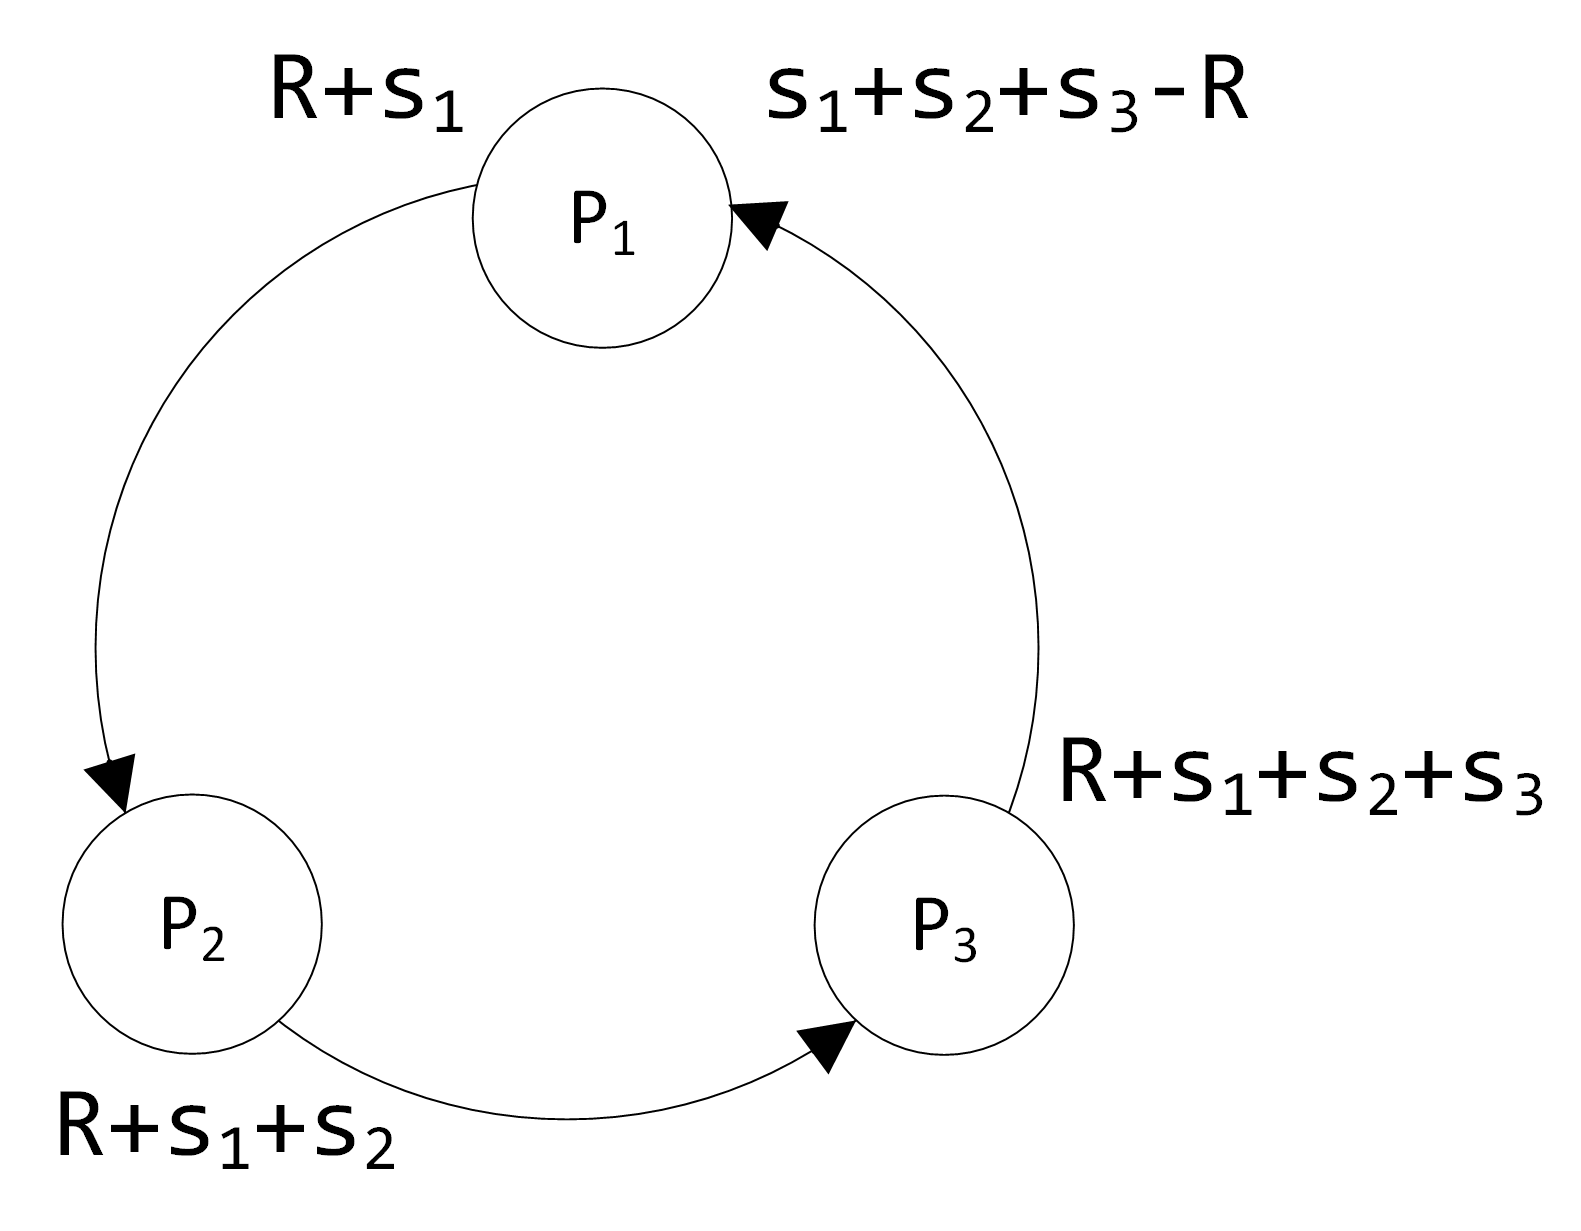
\includegraphics[scale=1.0]{figures/smpc-sum-simple-ring.png}
\end{figure}

This method is efficient ($2n$ messages for computation and announcing the sum in a $n$-node ring) but if parties collude, party $P_i$ only needs the output of $P_{i+1}$ as received by party $P_{i+2}$ to reconstruct the secret input of $P_{i+1}$. \textcite{Clifton2002} propose using shares in combination with permutation of the ring order, so neighbors change in each iteration and the number of parties in need to pool their data increases. This approach was extended in the "k-Secure Sum Protocol" \autocite{Sheikh2009}. Especially with a focus on security ($k\rightarrow n$) the permutation of the ring approaches share-exchanges between each node. To reduce the complexity through the ring permutation and motivated by the restrictions of the network (see \autoref{practicability of an implementation}), for which the protocol is intended, this thesis  uses a Shamir based protocol for a fully connected mesh network. 

In \ref{Secret Sharing} it was demonstrated how a secret can be reconstructed from the shares using Lagrange interpolation. It is also possible to reconstruct the sum of secrets by using the sums of shares for a Lagrange interpolation.

Proof:

$n$ shares for $m$ secrets $s_l$:
\begin{alignat}{1}
&s_{l,i} = f_l(x_i) = s_l + \sum_{i=1}^{k-1} \alpha_{l,i} x_i^i \mod p \\
& \Leftrightarrow \begin{cases}
s_{1,i} = f_1(x_i) = & s_1 + \alpha_{1,1} x_i + \alpha_{1,2} x_i^2 + ... + \alpha_{1,k-1}x_i^{k-1} \mod p \\
&\vdots \\
s_{m,i} = f_n(x_i) = & s_n + \beta_{n,1} x_i + \beta_{n,2} x_i^2 + ... + \beta_{n,k-1}x_i^{k-1} \mod p
\end{cases} \nonumber \\
& \text{with} \ \{l \in \gls{doubleN} \ | \ 1 \leq l \leq m \},
\ \{i \in \gls{doubleN} \ | \ 1 \leq i \leq n \},
\ \{ p \in \gls{doubleP} \ | \ p > \sum_l s_l \}, \nonumber \\
&\{ \alpha \in \gls{doubleN} \ | \ 0 \leq \alpha \leq p \},
\ \{k \in \gls{doubleN} \ | \ 2 < k \leq n \} \nonumber
\end{alignat}

Lagrange-interpolation for secret $s_l$:
\begin{alignat}{1}
&s_l = \sum_{i=1}^{n}s_{l,i}\prod_{i\neq j}\frac{-x_j}{x_i - x_j} \mod p \label{eq:Lagrange for s_l}
\end{alignat}
Sum $s$ over secrets $s_l$:
\begin{alignat}{1}
&s = \sum_{l=1}^{m} s_l \overset{\text{with} \ \ref{eq:Lagrange for s_l}}{=} \sum_{l=1}^{m} \sum_{i=1}^{n} s_{l,i}\prod_{i\neq j} \frac{-x_j}{x_i-x_j} \mod p \label{eq:sum over secrets}
\end{alignat}
\begin{alignat}{1}
&\text{with} \quad \sum_{i=1}^{n}\sum_{j=1}^{m}a_{ij} = \sum_{j=1}^{m}\sum_{i=1}^{n}a_{ij} \quad \text{follows for \ref{eq:sum over secrets}} \nonumber\\
&s= \underbrace{ \sum_{i=1}^n \underbrace{\sum_{l=1}^{m} s_{l,i}}_{\text{sum over shares}} \prod_{i\neq j} \frac{-x_j}{x_i-x_j} \mod p }_{\text{Lagrange-interpolation for sum over shares}}
\end{alignat}	

\subsubsection*{Example Computation}
Public information: $n=4$, $p=67$, $k=4$\par

\noindent Secrets: $s_1=13$, $s_2=27$, $s_3=17$, $s_4=1$\par

\noindent Target computation: sum $s$ over secrets $s= \sum_{i=1}^4 s_i=58$ without revealing ones secret to another party.		
\begin{alignat}{1}
s_{1,i}&=f_1(x_i)=13 + 35x + 22x^2 + 7x^3 \mod 67 \label{eq:example shares 1,i} \\
s_{2,i}&=f_2(x_i)=27 + 3x + 19x^2 \mod 67 \label{eq:example shares 2,i} \\
s_{3,i}&=f_3(x_i)=17 + 9x^2 + 27x^3 \mod 67 \label{eq:example shares 3,i} \\
s_{4,i}&=f_4(x_i)=1 + 13x + 31x^2 + 40x^3 \mod 67 \label{eq:example shares 4,i}
\end{alignat}
with $x_1=1$, $x_2=2$, $x_3=3$, $x_4=4$ follows
\begin{alignat}{7}
\overset{\ref{eq:example shares 1,i}}{\Rightarrow} s_{1,1}&=10 \quad &&s_{1,2}&&=26 \quad &&s_{1,3}&&=36 \quad  &&s_{1,4}&&=15  \nonumber \\
\overset{\ref{eq:example shares 2,i}}{\Rightarrow} s_{2,1}&=49 \quad &&s_{2,2}&&=42 \quad &&s_{2,3}&&=6 \quad &&s_{2,4}&&=8  \nonumber \\
\overset{\ref{eq:example shares 3,i}}{\Rightarrow} s_{3,1}&=53 \quad &&s_{3,2}&&=1 \quad &&s_{3,3}&&=23 \quad &&s_{3,4}&&=13  \nonumber \\
\overset{\ref{eq:example shares 4,i}}{\Rightarrow} s_{4,1}&=18 \quad &&s_{4,2}&&=2 \quad &&s_{4,3}&&=59 \quad &&s_{4,4}&&=27 \nonumber \\
\Rightarrow \sum_l s_{l,1}&=130 \quad \sum_l && s_{l,2}&&=71 \quad \sum_l && s_{l,3}&&=124 \quad \sum_l && s_{l,4}&&=63 \nonumber		
\end{alignat}
Lagrange-interpolation:
\begin{alignat}{2}
s&= &&\sum_{i=1}^{4}\sum_{l=1}^{4}s_{l,i}\prod_{i \neq j} \frac{-x_j}{x_i-x_j}\mod 67 \nonumber \\
&= &&130\frac{-2}{1-2}\frac{-3}{1-3}\frac{-4}{1-4}+71\frac{-1}{2-1}\frac{-3}{2-3}\frac{-4}{2-4} \nonumber \\
& &&+124\frac{-1}{3-1}\frac{-2}{3-2}\frac{-4}{3-4}+63\frac{-1}{4-1}\frac{-2}{4-2}\frac{-3}{4-3}\mod 67 \nonumber \\
&=&& 527 \mod 67 = 58 = \sum_{i=1}^4 s_i \label{eq:example result lagrange}
\end{alignat}
As expected, the result of the Lagrange-interpolation for the sum over shares is equal to the sum over the initial secrets (compare \ref{eq:example result lagrange}).

\subsubsection*{Protocol Description}
Assumptions:
%\vspace{-\topsep}
\begin{itemize}
	%\itemsep-0.5em
	\item number of parties $n>2$
	\item secure communication channel
	\item no malicious adversaries
	\item upper bound of sum $s \leq b$ can be estimated, so a prime $p > b$ can be chosen 
\end{itemize}
The secure addition protocol, as used in this thesis, consists of six phases:
\begin{enumerate}
	%\itemsep-0.5em
	\item The coordinator announces the number of parties for the computation and the indexation of each party.
	\item Each party $j$ sends shares $s_{j,i}$ of the secret input $s_j$ to the other parties.
	\item Each party $i$ computes the sum over the received shares $s_{j,i}$.
	\item Each party sends the computed sum to the coordinator.
	\item The coordinator reconstructs the sum over the inputs using Lagrange-interpolation.
	\item The coordinator broadcasts the reconstructed sum.
\end{enumerate}

In total $(n+3)\cdot (n-1)=n^2+2n-3$ messages are exchanged, so the traffic increases with the number of parties squared. Selecting a lower threshold for the secret reconstruction $\frac{n}{2} \leq k<n$ lowers the total messages by $\Delta_{\text{messages}}=n^2-n(k-1)$.

For a secure channel this protocol is information-theoretically secure: independent from computation power an adversary with $m_\text{leaked}<k$ shares will gain no information regarding the inputs.

\todo*{secure addition with verification \autocite{Cramer2015}; number of messages}

\subsection{Secure Comparison Protocol}	\label{Secure Comparison Protocol}
The secure comparison protocol compares the secret inputs and provides the minimum or maximum in a set without revealing the inputs or the parties holding the minimum or the maximum.

The protocol is based on the privacy preserving protocol for maximum computation as described in \textcite{Hasan2013}. The general idea is to use bit-decomposition and utilize the secure addition protocol bit-wise. In iterations the secure-sum for the bits ($0 \lor 1$) of the secrets multiplied with a random value are computed, starting from the \gls{MSB}, limited by a predefined upper bound, to the \gls{LSB}. The announced sum gives each party the information that at least one party has this bit set, if the sum is unequal zero. If a party has this bit not set itself it has a lower value and commits only zeros in the following iterations. Storing the result of each iteration, the parties can reconstruct the maximum.
For finding the minimum the protocol from \textcite{Hasan2013} needs an extension as described in \ref{Protocol Extension for Minimum Determination}: inputs are negated (using the binary operation NOT), making the minimum in the set the largest value. Afterwards the maximum is determined as described above. Finally the found maximum is negated again to reconstruct the minimum in the set.

\subsubsection{Example Computation} \label{Secure Comparison Example}

Public information: $n=3$, $p=67$, $\mathbb{Z}_p=\{1,...,p-1\}$, $k=3$, $s_i<b=64$ (upper bound for secret value range) \par
\noindent Secrets: $s_1=13$, $s_2=27$, $s_3=17$ \par

\noindent Target computation: $\min(s_i)=13$, $\max(s_i)=27$

Since $64_{10}=1000000_2$ is defined as upper bound for the secret values the \gls{MSB} is the sixth bit (second column in table \ref{table:secure maximum binary representation of secrets}).

\begin{table}[!htb]
	\centering
	\caption{Binary representation of secrets $s_i$} \label{table:secure maximum binary representation of secrets}
	\begin{tabular}{|c|l|l|l|l|l|l|}
		\hline
		Decimal $s_{i,10}$ & \multicolumn{6}{l|}{Binary $s_{i,2}$} \\ \hline
		13                 & 0    & 0    & 1    & 1    & 0   & 1   \\ \hline
		27                 & 0    & 1    & 1    & 0    & 1   & 1   \\ \hline
		17                 & 0    & 1    & 0    & 0    & 0   & 1   \\ \hline
	\end{tabular}
\end{table}

Each party multiplies each bit with a random within $\mathbb{Z_p}$:

\begin{table}[!htb]
	\centering
	\caption{Randomized binary representation of secrets} \label{table:secure maximum randomized binary representation}
	\begin{tabular}{|c|l|l|l|l|l|l|l|l|l|l|l|l|}
		\hline
		Decimal $s_{i,10}$ & \multicolumn{6}{l|}{Binary $s_{i,2}$}  & \multicolumn{6}{l|}{Randomized} \\ \hline
		13                 & 0    & 0    & 1    & 1    & 0   & 1 & 0    & 0    & 45    & 61    & 0   & 57   \\ \hline
		27                 & 0    & 1    & 1    & 0    & 1   & 1 & 0    & 12    & 31    & 0    & 5   & 15   \\ \hline
		17                 & 0    & 1    & 0    & 0    & 0   & 1 & 0    & 24    & 0    & 0    & 0   & 9   \\ \hline
	\end{tabular}
\end{table}

\begin{alignat}{3}
\intertext{There are six bits, therefore six rounds of secure addition ($\sum_{secure}$) are computed:}
1^{st} \ \text{round:} \quad & \sum_{secure}=0 && \Rightarrow \quad 6^{th} \ \text{bit of the maximum is} && 0 \nonumber \\
2^{nd} \ \text{round:} \quad &\sum_{secure}=36 > 0 \quad && \Rightarrow \quad 5^{th} \ \text{bit of the maximum is} \quad && 1 \nonumber \\
\intertext{Party $p_1$ disqualifies itself as the maximum (see table \ref{table:secure maximum p1 not maximum})}
3^{rd} \ \text{round:} \quad &\sum_{secure}=31 > 0 && \Rightarrow \quad 4^{th} \ \text{bit of the maximum is} && 1 \nonumber \\
\intertext{Party $p_3$ disqualifies itself as the maximum (see table \ref{table:secure maximum p3 not maximum})}
4^{th} \ \text{round:} \quad &\sum_{secure}=0 && \Rightarrow \quad 3^{rd} \ \text{bit of the maximum is} && 0 \nonumber \\
5^{th} \ \text{round:} \quad &\sum_{secure}=5>0 && \Rightarrow \quad 2^{nd} \ \text{bit of the maximum is} && 1 \nonumber \\
6^{th} \ \text{round:} \quad &\sum_{secure}=15>0 && \Rightarrow \quad 1^{st} \ \text{bit of the maximum is} && 1 \nonumber
\end{alignat}

\begin{table}[!htb]
	\centering
	\caption{Secure maximum protocol example: $2^{nd}$ round} \label{table:secure maximum p1 not maximum}
	\begin{tabular}{|l|l|l|l|l|l|l|}
		\hline
		Decimal $s_{i,10}$ & \multicolumn{6}{l|}{Randomized} \\ \hline
		13                 & 0    & \textcolor{red}{\underline{0}}    & $\cancelto{\textcolor{red}{0}}{45}$    & $\cancelto{\textcolor{red}{0}}{61}$    & \textcolor{red}{0}   & $\cancelto{\textcolor{red}{0}}{57}$   \\ \hline
		27                 & 0    & 12    & 31    & 0    & 5   & 15   \\ \hline
		17                 & 0    & 24    & 0    & 0    & 0   & 9   \\ \hline
	\end{tabular}
\end{table}

\begin{table}[!htb]
	\centering
	\caption{Secure maximum protocol example: $3^{rd}$ round} \label{table:secure maximum p3 not maximum}
	\begin{tabular}{|l|l|l|l|l|l|l|}
		\hline
		Decimal $s_{i,10}$ & \multicolumn{6}{l|}{Randomized} \\ \hline
		13                 & 0    & 0    & 0    & 0    & 0   & 0   \\ \hline
		27                 & 0    & 12    & 31    & 0    & 5   & 15   \\ \hline
		17                 & 0    & 24    & \textcolor{red}{\underline{0}}    & \textcolor{red}{0}    & \textcolor{red}{0}   & $\cancelto{\textcolor{red}{0}}{9}$   \\ \hline
	\end{tabular}
\end{table}

In total, each party has the bits $0|1|1|0|1|1$ stored and can reconstruct the correct maximum $\max(s_i)=27$.

\subsubsection{Protocol Extension for Minimum Determination} \label{Protocol Extension for Minimum Determination}

Using the negation of the binary representation, the order of the corresponding values in decimal numeral system is inverted (compare table \ref{table:secure minimum negation}). The computation is then the same as for the maximum search. The reconstructed maximum is finally negated to result in $\min(s_i)$.

\begin{table}[!htb]
	\centering
	\caption{Negation of binary representation for minimum determination} \label{table:secure minimum negation}
	\begin{tabular}{|l|l|l|l|l|l|l|l|l|l|l|l|l|}
		\hline
		Decimal $s_{i,10}$ & \multicolumn{6}{l|}{Binary $s_{i,2}$}  & \multicolumn{6}{l|}{Negated $\bar{s}_{i,2}$} \\ \hline
		13                 & 0    & 0    & 1    & 1    & 0   & 1 & 1    & 1    & 0    & 0    & 1   & 0   \\ \hline
		27                 & 0    & 1    & 1    & 0    & 1   & 1 & 1    & \textcolor{red}{\underline{0}} & 0    & 1    & 0   & 0   \\ \hline
		17                 & 0    & 1    & 0    & 0    & 0   & 1 & 1    & \textcolor{red}{\underline{0}} & 1    & 1    & 1   & 0   \\ \hline
	\end{tabular}
\end{table}

In the second round booth $P_2$ and $P_3$ disqualify themselves as maximum. After six rounds each party holds: $1|1|0|0|1|0$ as the maximum (see red markings in table \ref{table:secure minimum negation}). Negated this gives the minimum as $0|0|1|1|0|1_2=13_{10}$ 

\FloatBarrier

\subsubsection{Protocol Description}
Assumptions:
% \vspace{-\topsep}
\begin{itemize}
	% \itemsep-0.5em
	\item number of parties $n>2$
	\item secure communication channel
	\item no malicious adversaries
	\item upper bound of sum $s \leq b$ can be estimated, so a prime $p > b$ can be chosen 
\end{itemize}
The secure comparison protocol, as used in this thesis, consists of the phases for secure addition within iterations for the bitwise length of a predefined upper bound for the inputs: 
\begingroup
\sloppy
\begin{enumerate}
	\item The coordinator announces the number of parties for the computation and the indexation of each party.
	\item For minimum-search: each party negates the secret input.
	\item For each bit in the secret input starting from \gls{MSB} to \gls{LSB} each party runs through iterations:
	\begin{enumerate}
		\item If input is flagged as lower than maximum, then use $s_j=0$ as the input. Otherwise multiply actual bit $b$ with a random value $R$: $s_j=b \cdot R$.
		\item Each party $j$ sends shares $s_{j,i}$ of the input $s_j$ to the other parties.
		\item Each party $i$ computes the sum over the received shares $s_{j,i}$.
		\item Each party sends the computed sum to the coordinator.
		\item The coordinator reconstructs the sum over the inputs using Lagrange-interpolation.
		\item The coordinator broadcasts the reconstructed sum.
		\item Each party stores if the sum for the bit was equal 0 (set bit 0) or unequal 0 (set bit 1).
		\item Each party compares if bit from the computed sum is greater than own bit. If so input is flagged as lower than maximum.
	\end{enumerate}
	\item For minimum-search: each party negates the stored sum-result.
\end{enumerate}
\endgroup

Note: the assumption $n>2$ for the secure addition and secure comparison protocols is not strict enough, if sum, $\min$ and $\max$ are computed for the same parties, since for $n=3$ the secret between minimum and maximum can be restored (for a honest majority the mapping of values to parties is still secure though).

\subsection{Existing Frameworks} \label{Existing Frameworks}

In this section a short overview over existing \gls{SMPC} solutions is given. While \gls{SMPC} is an intensely researched field, practical work is less common.

The following solutions were considered

\begin{itemize}
	\item MpcLib (see \textcite{Online:MpcLib})
	\item SEPIA (see \textcite{Online:Sepia})
	\item SPDZ (see \textcite{Online:SPDZ})
	\item Sharemind (see \textcite{Online:Sharemind})
	\item Enigma (see \textcite{Online:Enigma})
\end{itemize}

Some key-features of the solutions are illustrated in figure \ref{figure:existing frameworks}. All projects emerged from university research. With the exception of Sharemind and Enigma, the frameworks seem to target primarily other researchers, reflecting in the lack of documentation and thereby reduced usability. The open-source library MpcLib is C\# based, SPDZ uses C++ and Python and SEPIA is a Java library.  Sharemind and Enigma are also booth based on university research (Enigma at MIT and Sharemind at University of Tartu) but evolved into market-ready business solutions. While Sharemind uses dedicated application-server, Enigma uses a distributed system of nodes based on Blockchain technology for \gls{SMPC}, booth with a focus on scalable secure data analysis.
All solution are based on the Internet protocol suite and require at least locally run server or Internet access.

\begin{figure}[!htb] % h for placement here
	\caption{Existing \gls{SMPC} software grouped by properties} \label{figure:existing frameworks}
	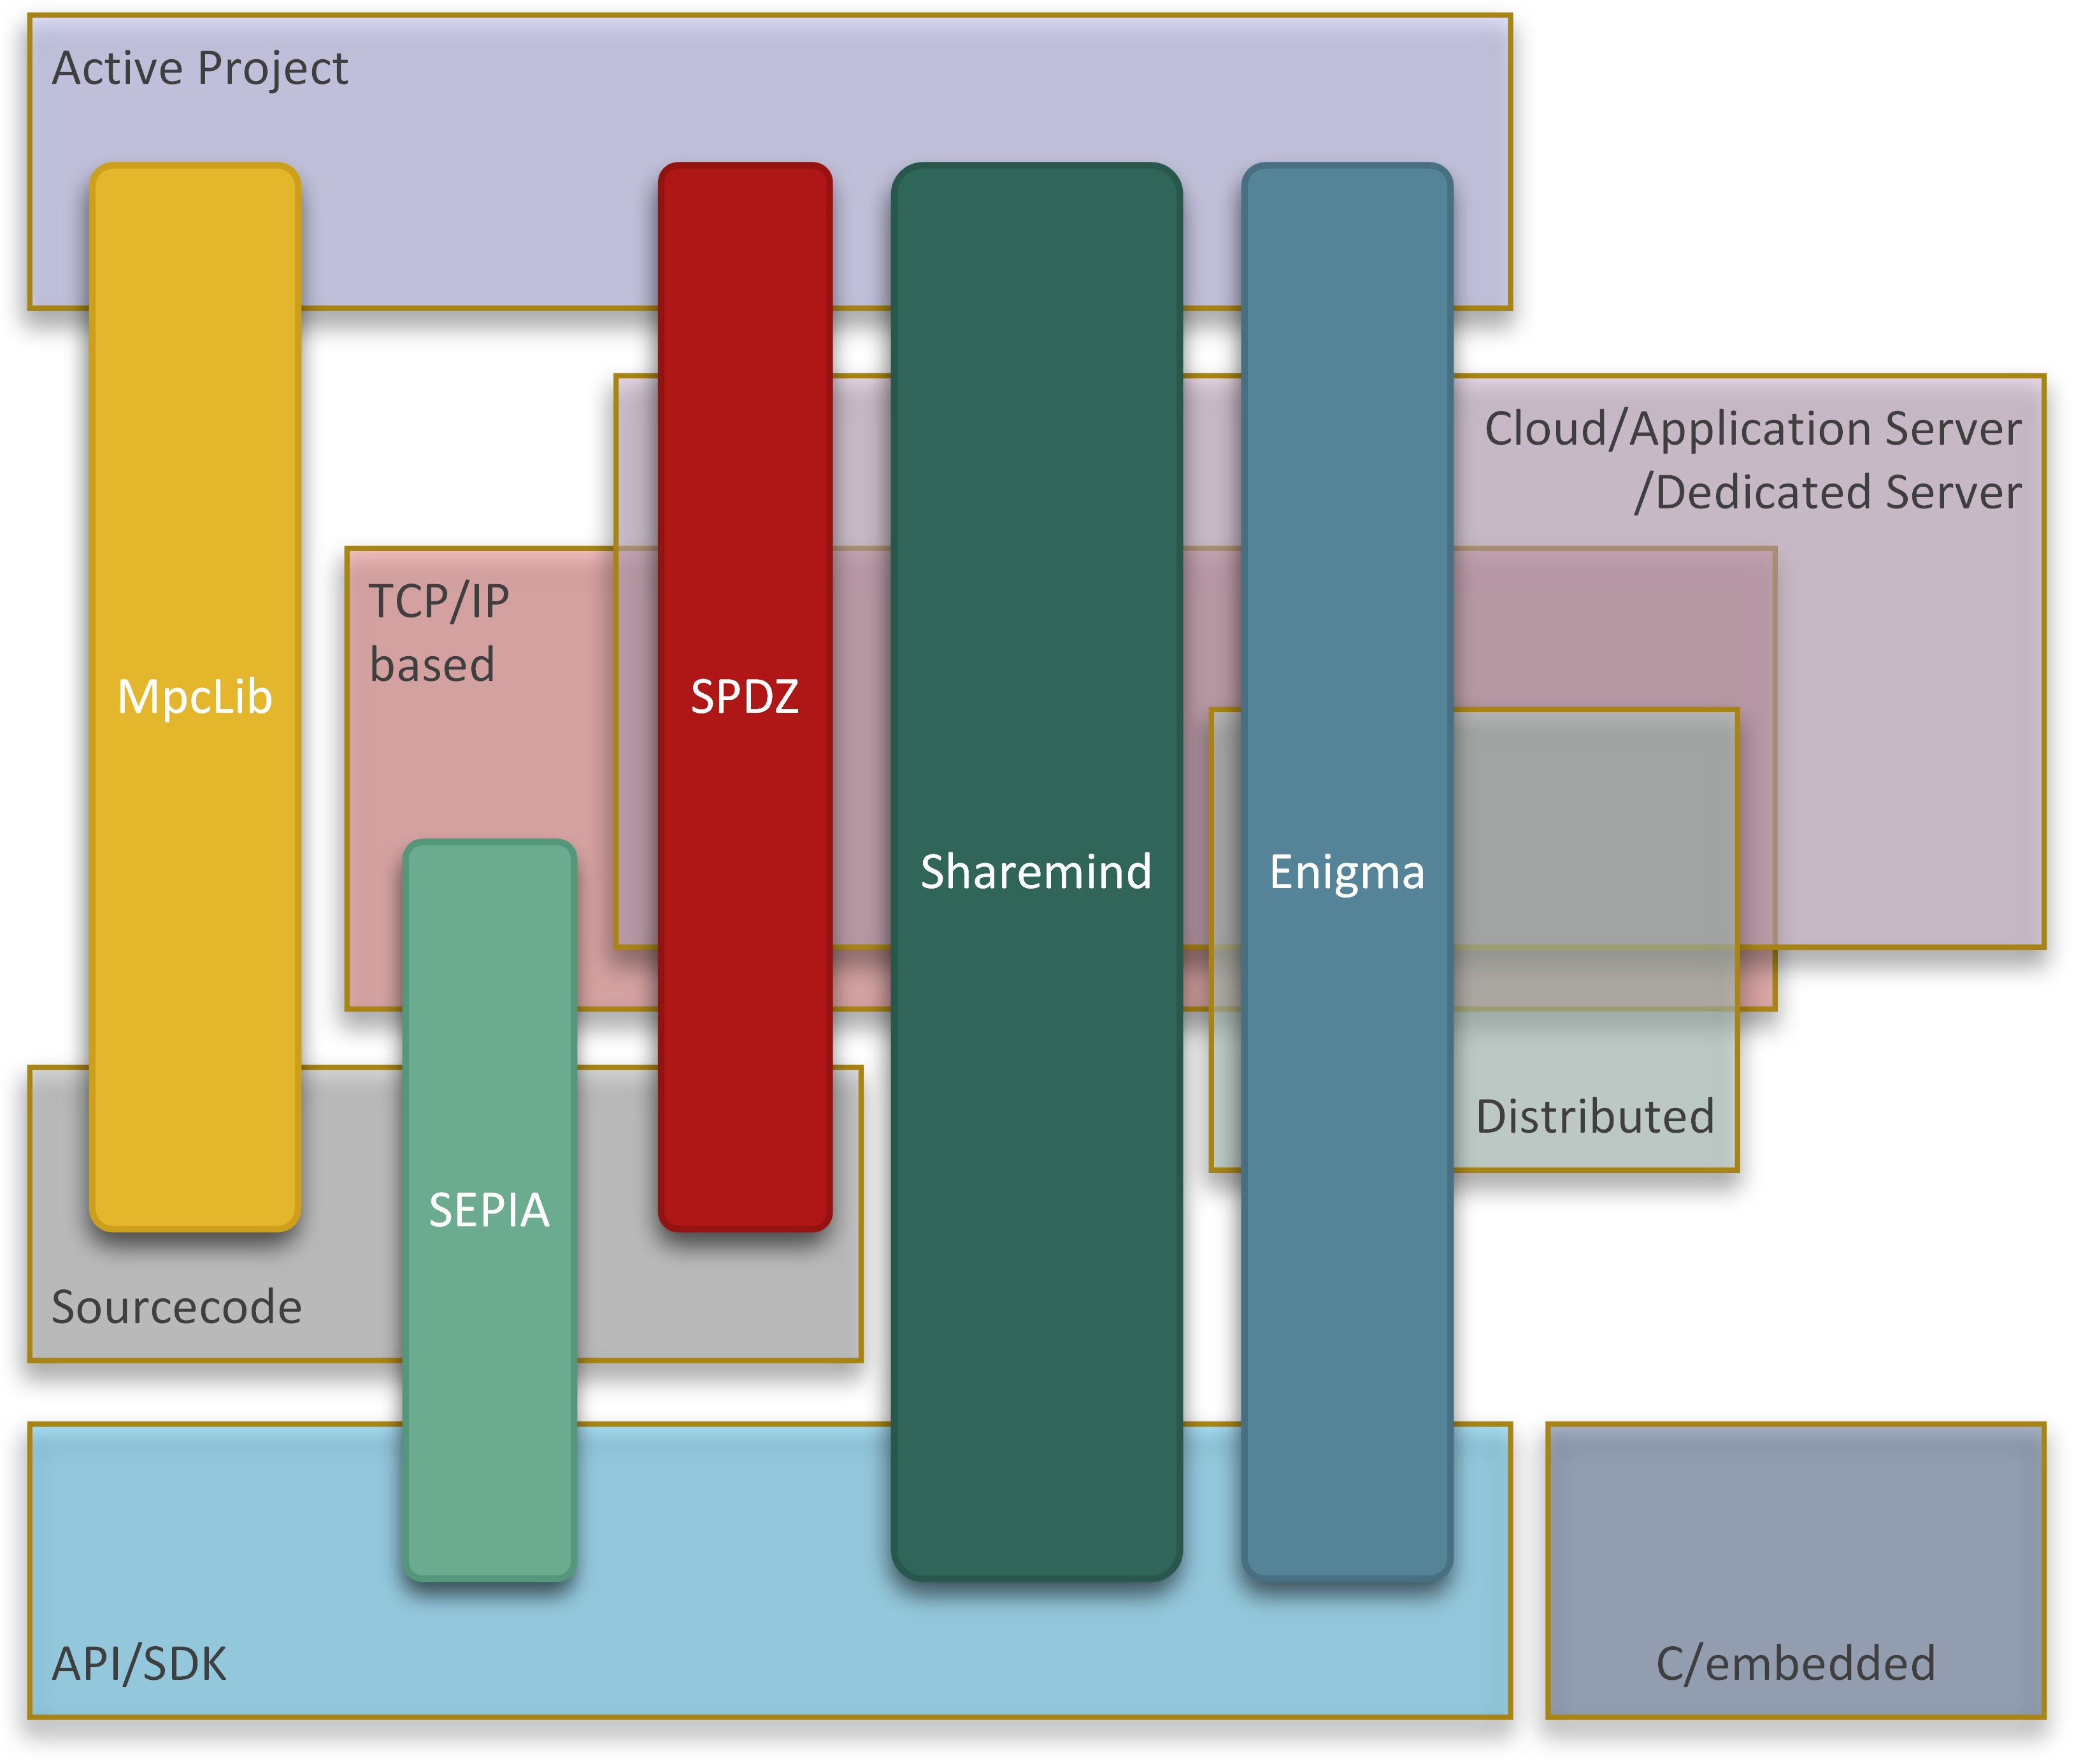
\includegraphics[scale=1.0]{figures/frameworks.png}
\end{figure}

While all frameworks exceed the requirements regarding the \gls{SMPC} functionality, they don't provide a solution for local ad-hoc networks without permanently available servers. Also the support for low-level devices is either undocumented or not given through programming language dependencies.
The development of a framework with a focus on cross-platform usage, usability for developers without cryptographic research background and applicability for local ad-hoc networks for the described gamification use-cases is therefore justified.

\FloatBarrier

\section{Mobile Ad Hoc Networks} \label{Mobile Ad Hoc Networks}
The framework developed as part of this thesis focuses on providing \gls{SMPC} for \glspl{MANET} or \gls{MANET}-like networks. In this section the network topologies related to \glspl{MANET} are briefly described (see \ref{Network Topologies}) and the practicability of an implementation based on current technology standards are examined (see \ref{practicability of an implementation}).

\subsection{Network Topologies} \label{Network Topologies}

\begingroup 
\sloppy
\textcite{Dorri2015} describe a \gls{MANET} as an "infrastructure-in\-de\-pen\-dent network with wireless mobile nodes" \autocite[p. 15]{Dorri2015}. A \gls{MANET} is similar to a mesh network, but the distinctive feature is the nodes' spatial degree of freedom. In comparison to a star network, there is no central switch dedicated to routing messages. Instead each node provides message passing abilities and acts as a multi-hop relay.
\endgroup
The advantage of \glspl{MANET} is the open network boundary: nodes can freely join and leaving nodes do not affect the functionality of the \gls{MANET}. The key-features are:

%\vspace{-\topsep}
\begin{itemize}  
	%\itemsep-0.5em
	\item continuously self-configuring
	\item self-forming
	\item self-healing
	\item infrastructure-less
	\item peer-to-peer
	\item  mobility of nodes (main difference to mesh network)
\end{itemize}

The message passing in a \gls{MANET} can either be done by routing or flooding. Since the nodes can move freely, the neighbors will change often, so maintaining routing tables is expensive. The passing of messages without the availability of authentication protocols like \gls{HTTPS} makes the communication also vulnerable against man-in-the-middle attacks. Of course flooding means broadcasting and is not cheap either in regard to message quantity and network load.

The mentioned key-features of \glspl{MANET} make it a good network choice for a gamification setting based on mobile devices (smartphones, wearables, etc.), because it promises unobtrusive usage for participants without administrative maintenance effort. In the next section the availability and the practicability of an implementation for Android devices is discussed, because of Androids dominant position as the globally leading smartphone \gls{OS} with a market share of above 80\% (see \textcite{Online:Gartner2016}). 

\subsection{Practicability of an implementation on Android Devices} \label{practicability of an implementation}

\glspl{MANET} are especially of interest for military applications and disaster management but they are also gaining research focus for civil usage for example in context of \gls{IoT} devices. Demonstrations of an implementation can be found for example in Open Gardens MeshKit \gls{SDK} \autocite{Online:MeshKit}, which offers \gls{MANET} abilities for Android and iOS devices and thereby forming a \gls{SPAN}. MeshKit is also the foundation for Open Gardens FireChat \autocite{Online:FireChat}, which is for example known in context of pro-democracy demonstrations. Since Android does not provide an \gls{API} for \gls{MANET} functionality on Android devices (\gls{API} 24 at the time of writing) and the MeshKit \gls{SDK} is not open source and only available through Open Gardens partner program, a simplified (but extendable) implementation of \gls{MANET}-like behavior is developed in the application layer (compare \ref{Coordinator Election}).
Both for Wi-Fi and Bluetooth based connections, there can be limitations in regard to maximum concurrent connections. Vendor specific restrictions (hardware, driver) are hard to compensate reactive at runtime, so this issue has to be addressed proactive in \ref{Architecture} \nameref{Architecture}.

\subsubsection{Bluetooth Based \gls{MANET}}

Usually Bluetooth connections with smartphones require pairing and user actions. This is not a useful process flow to build a \gls{MANET}-like network, since nodes cannot simply join.
Using the Bluetooth protocol \gls{RFCOMM} an insecure connection can be established, without the need for pairing and user interaction. \textcite{RFCOMM2012} describe \gls{RFCOMM} as the emulation of serial ports over \gls{L2CAP}, supporting the emulation of multiple ports between two devices and ports between multiple devices (device dependent).
Since multiple simultaneous connection have to share the available bandwidth per node, it takes $\frac{n}{2}$ times longer to share the same amount of data when using only one-to-one connections sequentially. For the targeted number of computation partners in this thesis, this is a tolerable overhead and practical system parameters will be evaluated in \autoref{Evaluation} and \autoref{Discussion}.
The Bluetooth Special Interest Group has announced mesh networking protocols for upcoming specifications \autocite{Online:BluetoothMesh}. This is very promising in regard of system provided \gls{MANET} features, though it will take time (from experience with Bluetooth LE likely years) until enough devices are equipped with compliant Bluetooth modules.

\subsubsection{Wi-Fi Based \gls{MANET}}

Situations in which we can use Wi-Fi (or \gls{GSM}) usually provide Internet access, so Wi-Fi is not the primary target technology for this thesis. Generally, the callback-based architecture of the developed framework (compare \ref{Architecture} \nameref{Architecture}) enables the usage of different wireless technologies though. Even the interconnection of \gls{MANET}-like networks is conceivable (as demonstrated with MeshKit), but it complicates the forming of the computation group (compare \ref{Coordinator Election}), because different optional channels between nodes have to be evaluated.
With Android 4.0 (\gls{API} level 14) the Wi-Fi Peer-to-Peer framework was introduced, which complies with the Wi-Fi Alliance's Wi-Fi Direct certificate program. Wi-Fi Direct states that one-to-one or group (many-to-one) connections are possible. One device acts as a group owner (soft access point), so it forms a star topology. To imitate a \gls{SPAN} with Wi-Fi Direct multi-group communication has to be provided. In \textcite{Funai2015} limitations of Android in regard of multi-group networking as well as solutions are discussed.
Other solutions (compare \textcite{Online:SPANProject}) include usage of custom kernels on rooted smartphones. Even though  demonstrations on selected devices have shown the feasibility, such system modifications neglect the target group and the intentions of this framework.

%\section{Pseudo-Random Numbers} %maybe move to implementation/secureing channel
%\label{sec:Pseudo-Random Numbers}

%\todo*{random numbers important for cryptography: selection of coefficients in secret sharing, public key generation, ...; RNG in different environments; entropy}

%https://en.wikipedia.org/wiki/Cryptographically_secure_pseudo-random_number_generator

%\todo*{lib will require a callback for random number generator -> maybe mention with outlook for requirements}

\FloatBarrier

\chapter{Design} \label{Design}

\todo*{15-20\%; explains complete processing chain; explains what methods are used; for someone that wants to know what was done in detail}

Based on the findings in chapter \fullref{Background} and extended with use-cases the requirements for the framework are specified in \fullref{Requirements}. In \fullref{Decentralized, Distributed Computing} specific requirements in context of complex processes are substantiated with algorithms for decentralized, distributed computing. Finally, a draft design is presented in \fullref{Architecture}.

\section{Requirements} \label{Requirements}

In general this thesis follows the FURPS+ system for requirements as described by \textcite{Online:FURPS}: 
requirements are categorized into functional and non-functional requirements:
\begin{alignat*}{1}
& \begin{rcases*}
\mathmakebox[\widthof{\text{Supportability}}][l]{\text{Functionality}} & \quad
\end{rcases*} \mathmakebox[\widthof{\text{non-functional requirements}}][l]{\text{functional requirements}} \\
& \begin{rcases*}
\text{Usability} & \quad \\
\text{Reliability} & \quad \\
\text{Performance} & \quad \\
\text{Supportability} & \quad
\end{rcases*} \text{non-functional requirements}
\end{alignat*}

The functional and non-functional requirements are specified in \ref{Functional Requirements} and \ref{Non-Functional Requirements}. 

\subsection{Functional Requirements} \label{Functional Requirements}

Functional requirements define the functions the framework has to offer to meet the acceptance criteria. Based on chapter \fullref{Background} we can divide the requirements into two main fields: features regarding the accurate computation of the \gls{SMPC} protocols and functions required to compensate the lack of a \gls{MANET} \gls{API} and technical limitations.
Figure \ref{figure:requirements use-case node} presents the general functionality a party - respectively a node - expects from the system: especially the need for a secure channel and the limitation to run the \gls{SMPC} only with nearby computation partners is caused by the missing multi-hop capabilities.

\begin{figure}[!htb] % h for placement here
	\caption[General functional requirements of a node]{\gls{UML} use-case diagram for the general functional requirements of a node} \label{figure:requirements use-case node}
	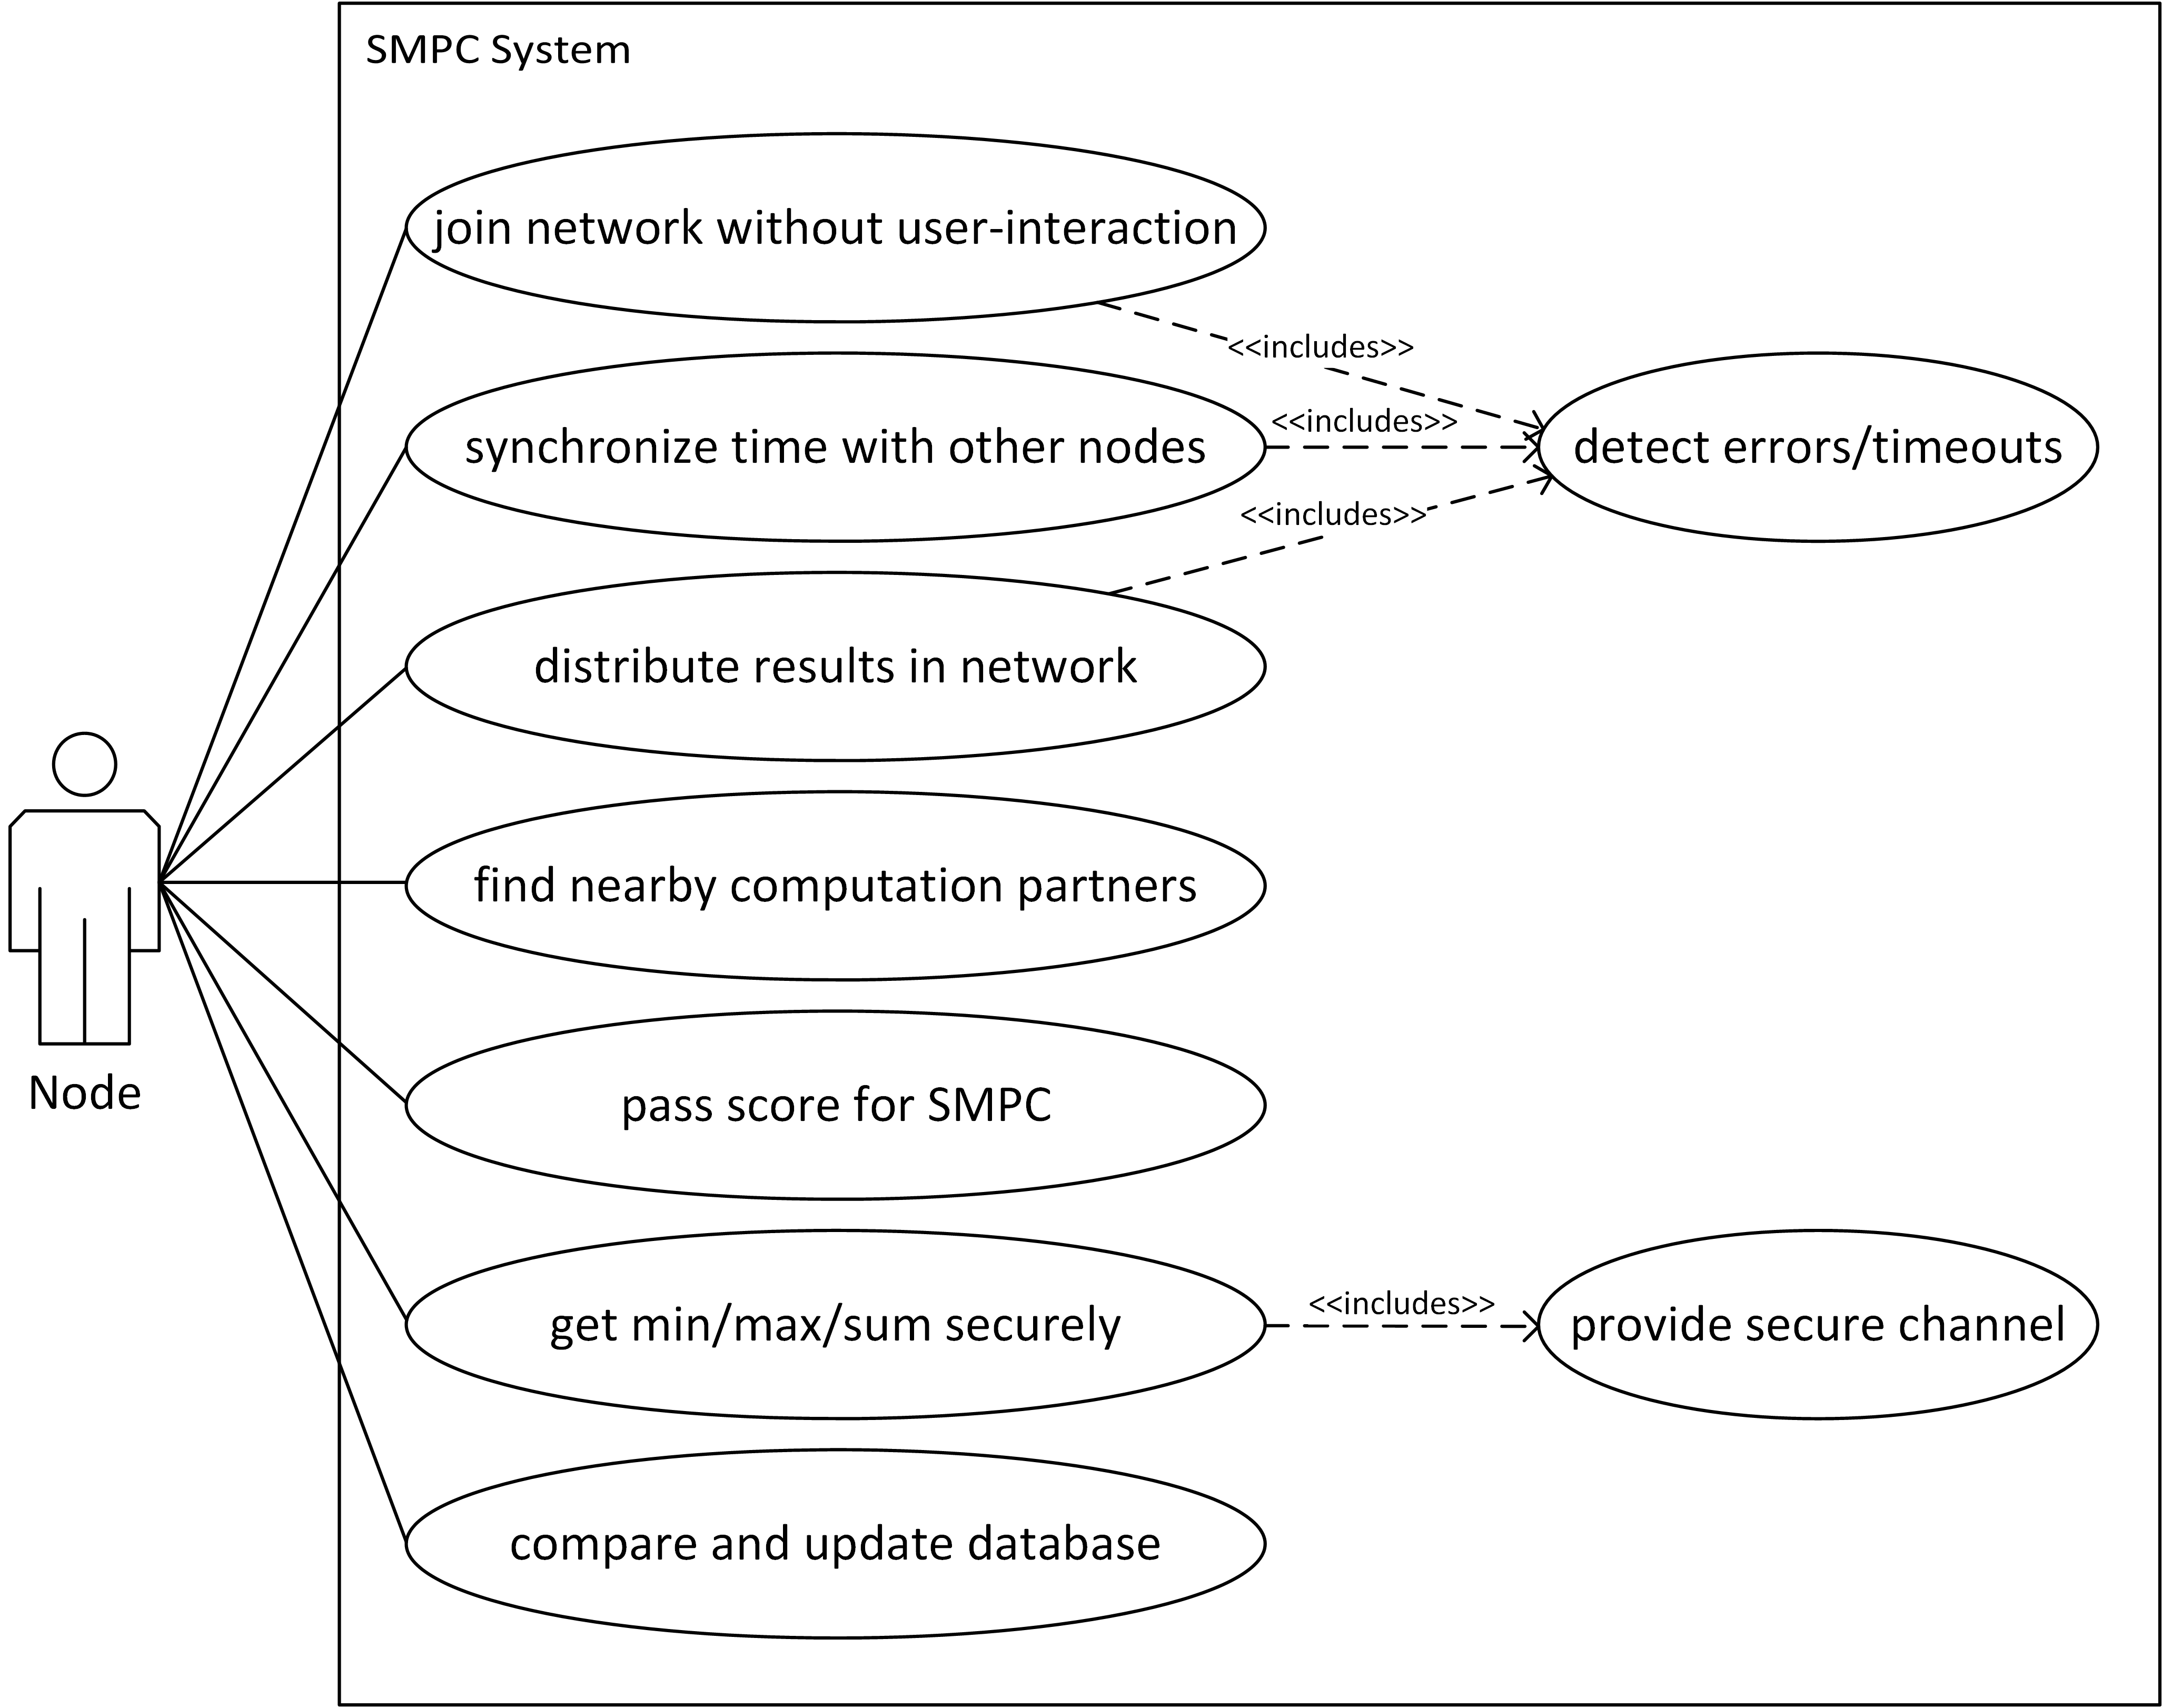
\includegraphics[scale=0.85]{figures/use-case-node.png}
\end{figure}

Since most functions (like the time synchronization and the multi-party computation) require the interaction between nodes, these processes need to be coordinated. In a distributed system there is no central authority, so a node has to become the temporal leader or coordinator for the duration of a process. In figure \ref{figure:requirements use-case coordinator} the processes requiring coordination are described as use-cases from the view of a temporal coordinator.

\begin{figure}[!htb] % h for placement here
	\caption[Use-case diagram for coordinator requirements]{\gls{UML} use-case diagram for the functional requirements for the coordinator} \label{figure:requirements use-case coordinator}
	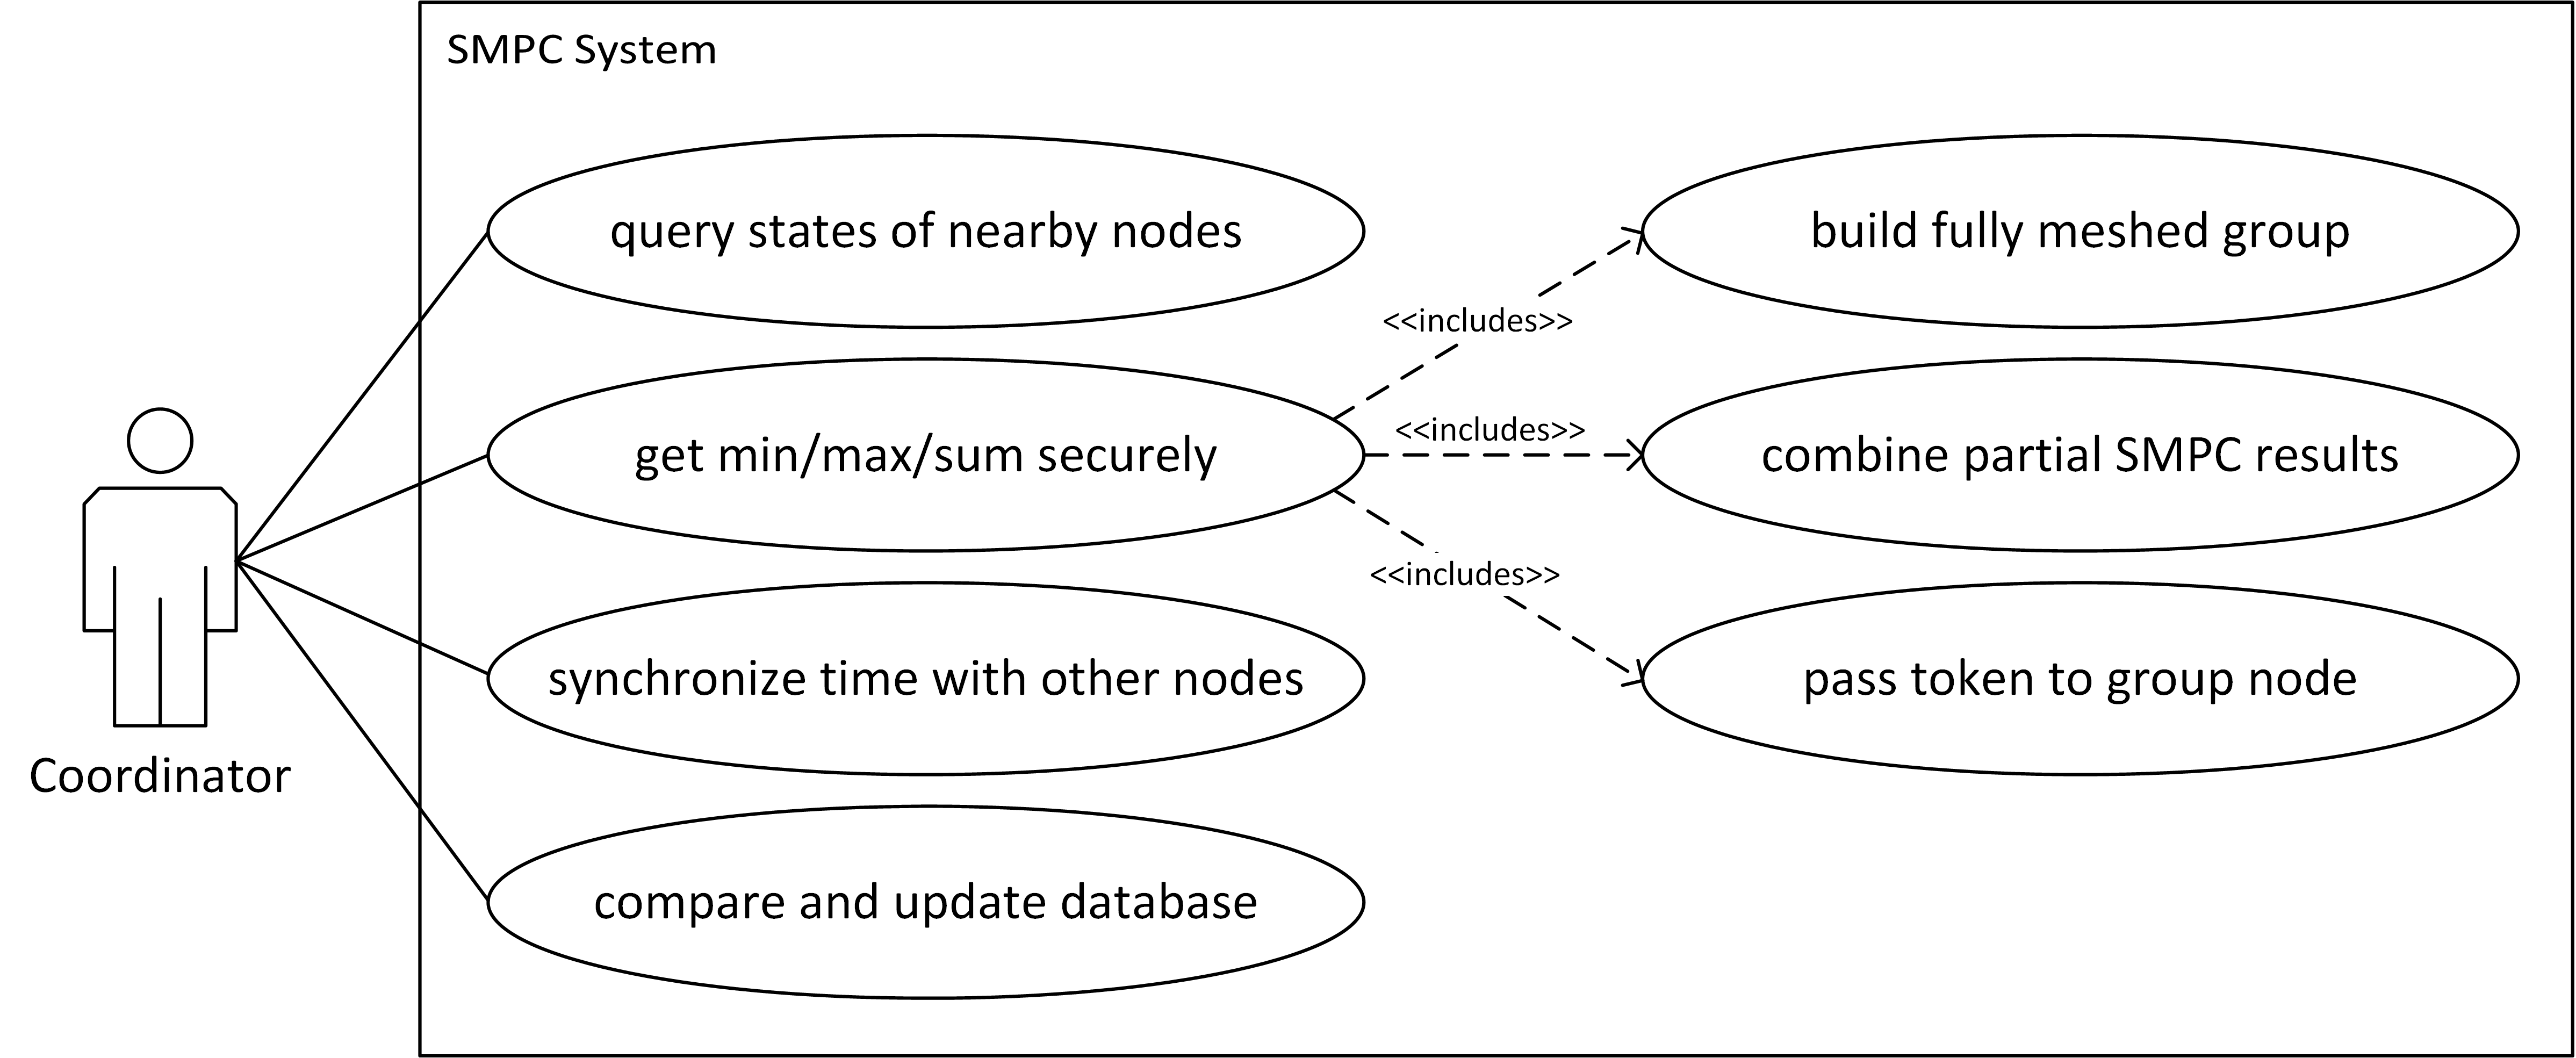
\includegraphics[scale=0.75]{figures/use-case-coordinator.png}
\end{figure}

Based on the use-cases functional requirements can easily be identified and specified. In table \ref{table:functional requirements} the functional requirements are stated as user-stories, alongside assumptions and targeted tests.


\begin{table}[!htb] % h for placement here
	\centering
	\caption{Functional requirements} \label{table:functional requirements}
	\begin{tabular}{|l|p{\textwidth*5/6-7mm}|}
		\toprule
		Name & \funcreq{Pairing-less Connection}\label{req:Pairing-less Connection} \\ \midrule
		Requirement & As a node I want to join the system without having to pair with other devices so that the system remains unobtrusive. \\
		Assumptions & Device has Bluetooth capabilities with \gls{RFCOMM} protocol. \\ \midrule
		Name & \funcreq{Heartbeat}\label{req:Heartbeat} \\ \midrule
		Requirement & As a node I need to inform my coordinator if my computation is running longer than expected so that the system does not assume that the process has failed. As a coordinator I need to inform all group nodes if a computation is running longer than expected. \\
		Assumptions & Hosting system provides system time. \\ \midrule
		Name & \funcreq{Non-termination Detection}\label{req:Non-termination Detection} \\ \midrule
		Requirement & As a node I must be able to detect a communication problem so that I can reset my status. \\
		Assumptions & Hosting system provides system time. \\ \midrule
		Name & \funcreq{Coordinator Election}\label{req:Coordinator Election} \\ \midrule
		Requirement & As a node I want to become coordinator for nearby nodes so that communication can be organized. \\ \midrule
		Name & \funcreq{Token-Passing}\label{req:Token-Passing} \\ \midrule
		Requirement & As coordinator I want to be able to assign a group-member to coordinate a subprocess so that direct communication between group-members can be established. \\ \midrule
		Name & \funcreq{Secure Multi-Party Computation Module}\label{req:SMPC Module} \\ \midrule
		Requirement & As a coordinator I want to form a group of fully meshed nodes and coordinate the execution of the secure addition and secure comparison protocols using a secure communication channel. \\ \todo*{visualize finding fully-meshed nearby group in mesh network}
		Assumptions & Group size $>2$. All group-members are time-synchronized and have a score within the same time-frame limits. \\
		Testability & Unit tests to proof correctness of implementation. Performance-tests with different number of computation partners and validation of result. \\ \midrule
		Name & \funcreq{Clock Synchronization}\label{req:Clock Synchronization} \\ \midrule
		Requirement & As coordinator I want to synchronize the clocks of nearby nodes so that computation results are not biased because of different time settings. \\
		Testability & Unit tests to proof correctness of implementation. \\ \midrule
		Name & \funcreq{Database Synchronization}\label{req:Database Synchronization} \\ \midrule
		Requirement & As coordinator I want to compare my database status with nearby nodes and exchange missing entries without having to compare all entries. \\
		Assumptions & Participating nodes are idle and not waiting for a computation.\\
		\bottomrule
	\end{tabular}
\end{table}

\subsection{Non-Functional Requirements} \label{Non-Functional Requirements}

Non-functional requirements describe quality attributes the system has to comply to. Two use-cases from a developer view are illustrated in figure \ref{figure:requirements use case developer}.

\begin{figure}[!htb] % h for placement here
	\caption{\gls{UML} use case diagram for developer} \label{figure:requirements use case developer}
	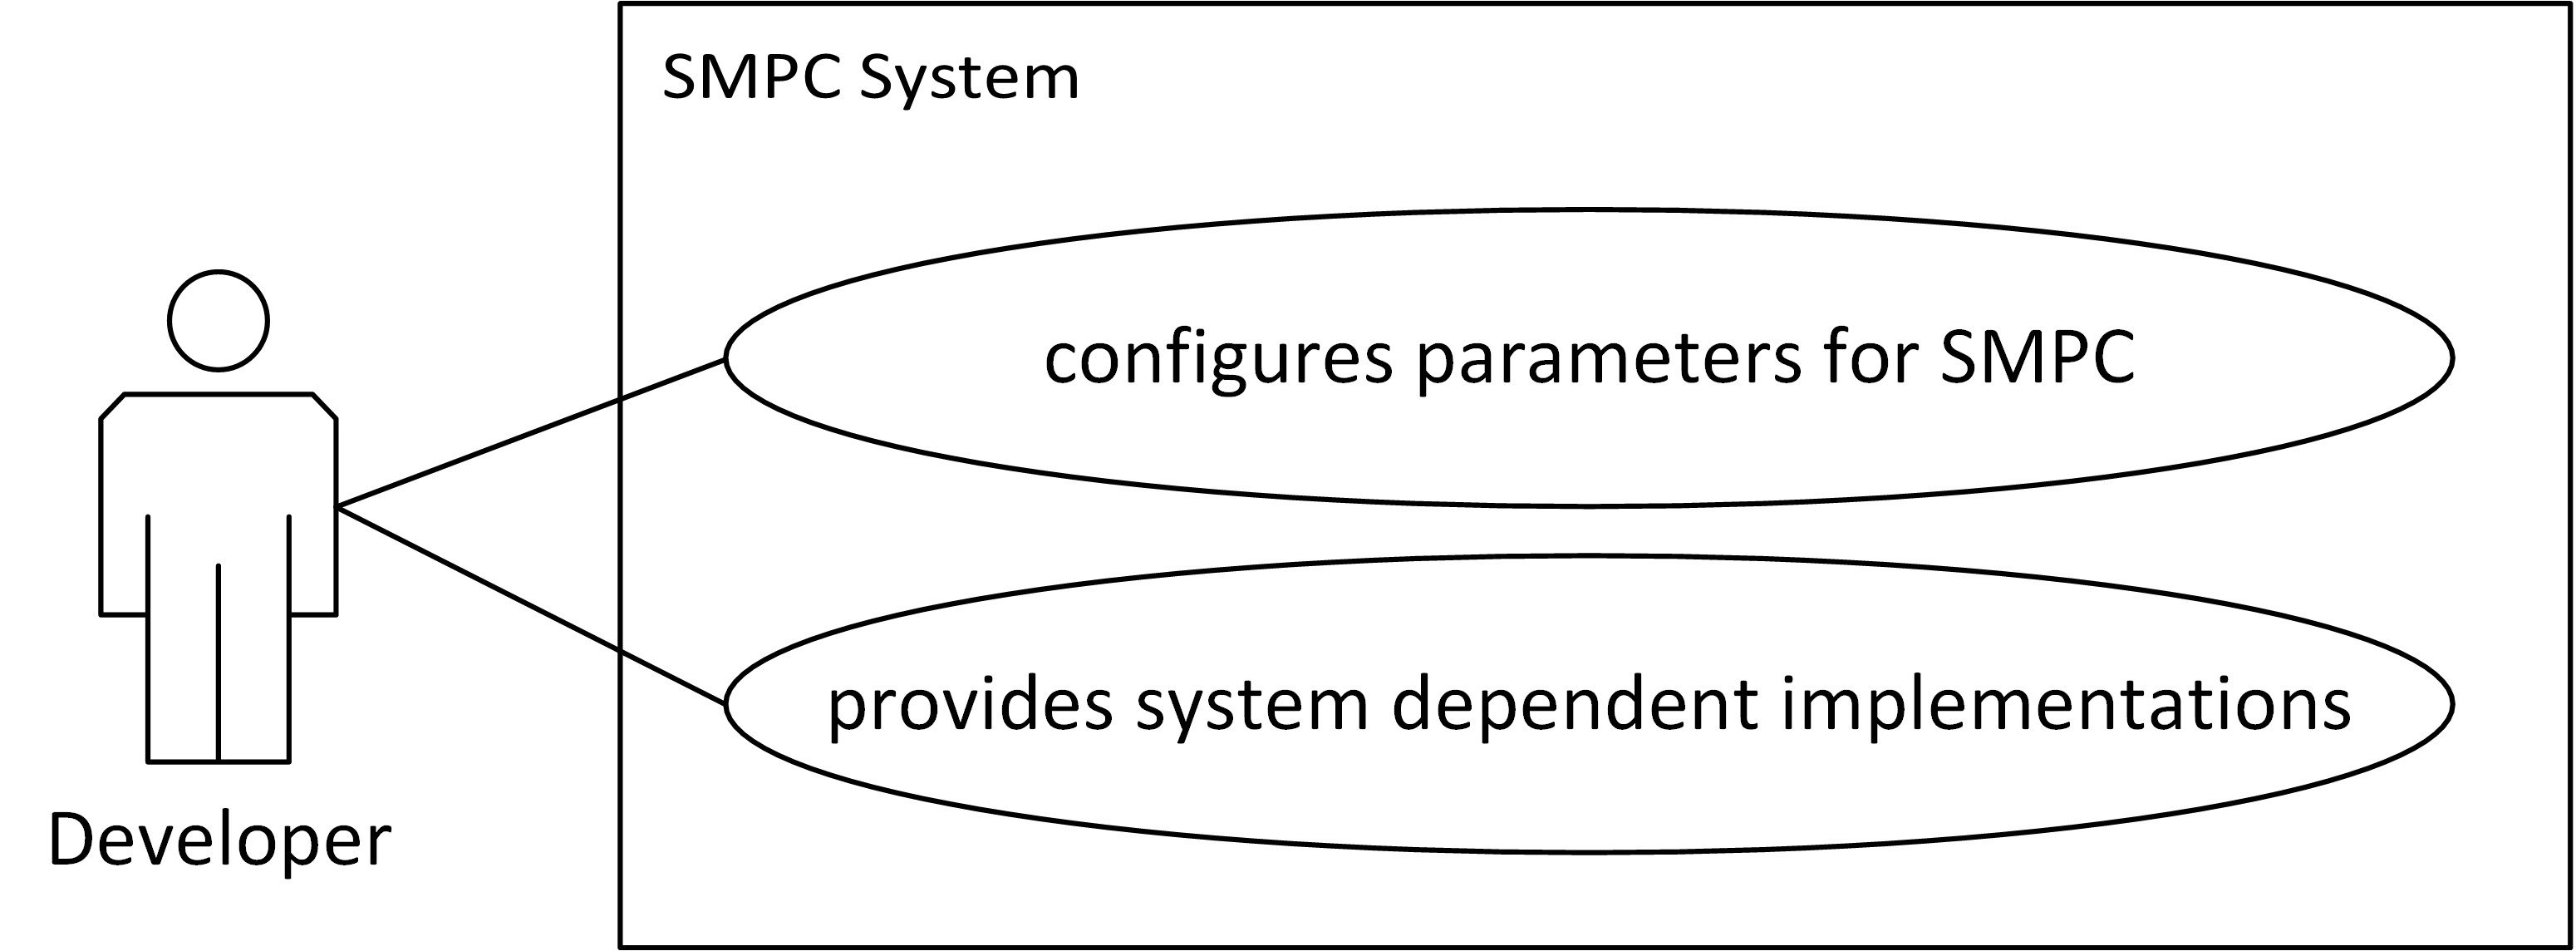
\includegraphics[scale=0.85]{figures/use-case-developer.png}
\end{figure}

Based on the use-cases for developers and general demands regarding the maintainability, expandability and performance to make the framework applicable for real-life settings, non-functional requirements can be specified as listed in table \ref{table:non-functional requirements}.

\begin{table}[!htb] % h for placement here
	\centering
	\caption{Non-functional requirements} \label{table:non-functional requirements}
	\begin{tabular}{|l|p{\textwidth*4/5}|}
		\toprule
		Name & \nonfuncreq{Usability}\label{req:Usability} \\ \midrule
		Requirement & The framework shall be configurable, so that a developer using the framework can configure the settings for the \gls{SMPC}. \\ \midrule
		Name & \nonfuncreq{Maintainability}\label{req:Supportability} \\ \midrule
		Requirement & The framework shall be maintainable, so that the code and documentation make it clear for a developer what callbacks have to be implemented and how the framework can be used in an Android device. \\ \midrule
		Name & \nonfuncreq{Performance}\label{req:Performance} \\ \midrule
		Requirement & The framework shall be secure while providing enough performance, that computations can properly terminate for nodes that move at walking speed ($\approx1\frac{m}{s}$). \\ \midrule
		Name & \nonfuncreq{Expandability}\label{req:Expandability} \\ \midrule
		Requirement & The frameworks coupling with the wireless technology shall be loosely, so that the system can be extended without having to touch core functionalities regarding the \gls{SMPC}.  \\ \bottomrule
	\end{tabular}
\end{table}

\section{Decentralized, Distributed Computing} \label{Decentralized, Distributed Computing}

While the protocols for secure addition and secure comparison and thereby the requirement \ref{req:SMPC Module} are already well-defined (compare \autoref{Secret Sharing}, \autoref{Secure Addition Protocol} and \autoref{Secure Comparison Protocol}), other functional requirements need further methodical substantiation. \ref{req:Coordinator Election} and \ref{req:Token-Passing} are addressed in \autoref{Coordinator Election}, \ref{req:Heartbeat} and \ref{req:Non-termination Detection} are discussed in \autoref{Non-termination Detection}, an algorithm for \ref{req:Clock Synchronization} is provided in \autoref{Clock synchronization} and finally \ref{req:Database Synchronization} is covered in \autoref{Distributed Database}.

\subsection{Coordinator Election and Coordinator Role} \label{Coordinator Election}

As discussed in \autoref{practicability of an implementation} fully featured \glspl{MANET} are currently not provided and mapping it completely in the application layer is beyond the scope of this thesis. Overcoming the technical limitations, the system can be build with sequential communications instead of parallel. As stated in \fullref{Network Topologies} communication in context of \glspl{SMPC} is only done in a fully meshed subgroup of the network, which also simplifies the coordinator election.

\noindent A node will try to become the coordinator, when \nolinebreak
%\vspace{-\topsep}
\begin{enumerate}
	%\itemsep-0.5em
	\item it enters the network after longer disconnection: event driven.
	\item a new personal score is ready for \gls{SMPC}: event driven.
	\item all \gls{SMPC} computations for a score are done: event driven.
	\item an event driven attempt failed and a certain amount of time passed: timer based.
\end{enumerate}

Extending requirement \ref{req:Coordinator Election} and to avoid situations of competing nodes trying to become coordinator and thereby booth repeatedly failing because neither can acquire enough computation partners, the timer based approach is supported by the exponential backoff algorithm. \textcite[p.67]{IEEE2010} describe the exponential backoff algorithm for collision detection and retransmission: if a coordinator appointment failed (equivalent to collision detection in original description) a factor for the waiting time till the next attempt is selected uniformly random from an increasing range, reducing the probability for competing coordinator candidates. The process is outlined in form of an \gls{UML} activity diagram in figure \ref{figure:coordinator exponential backoff}.

\begin{figure}[htbp] % h for placement here
	\caption{\gls{UML} activity diagram for exponential backoff algorithm} \label{figure:coordinator exponential backoff}
	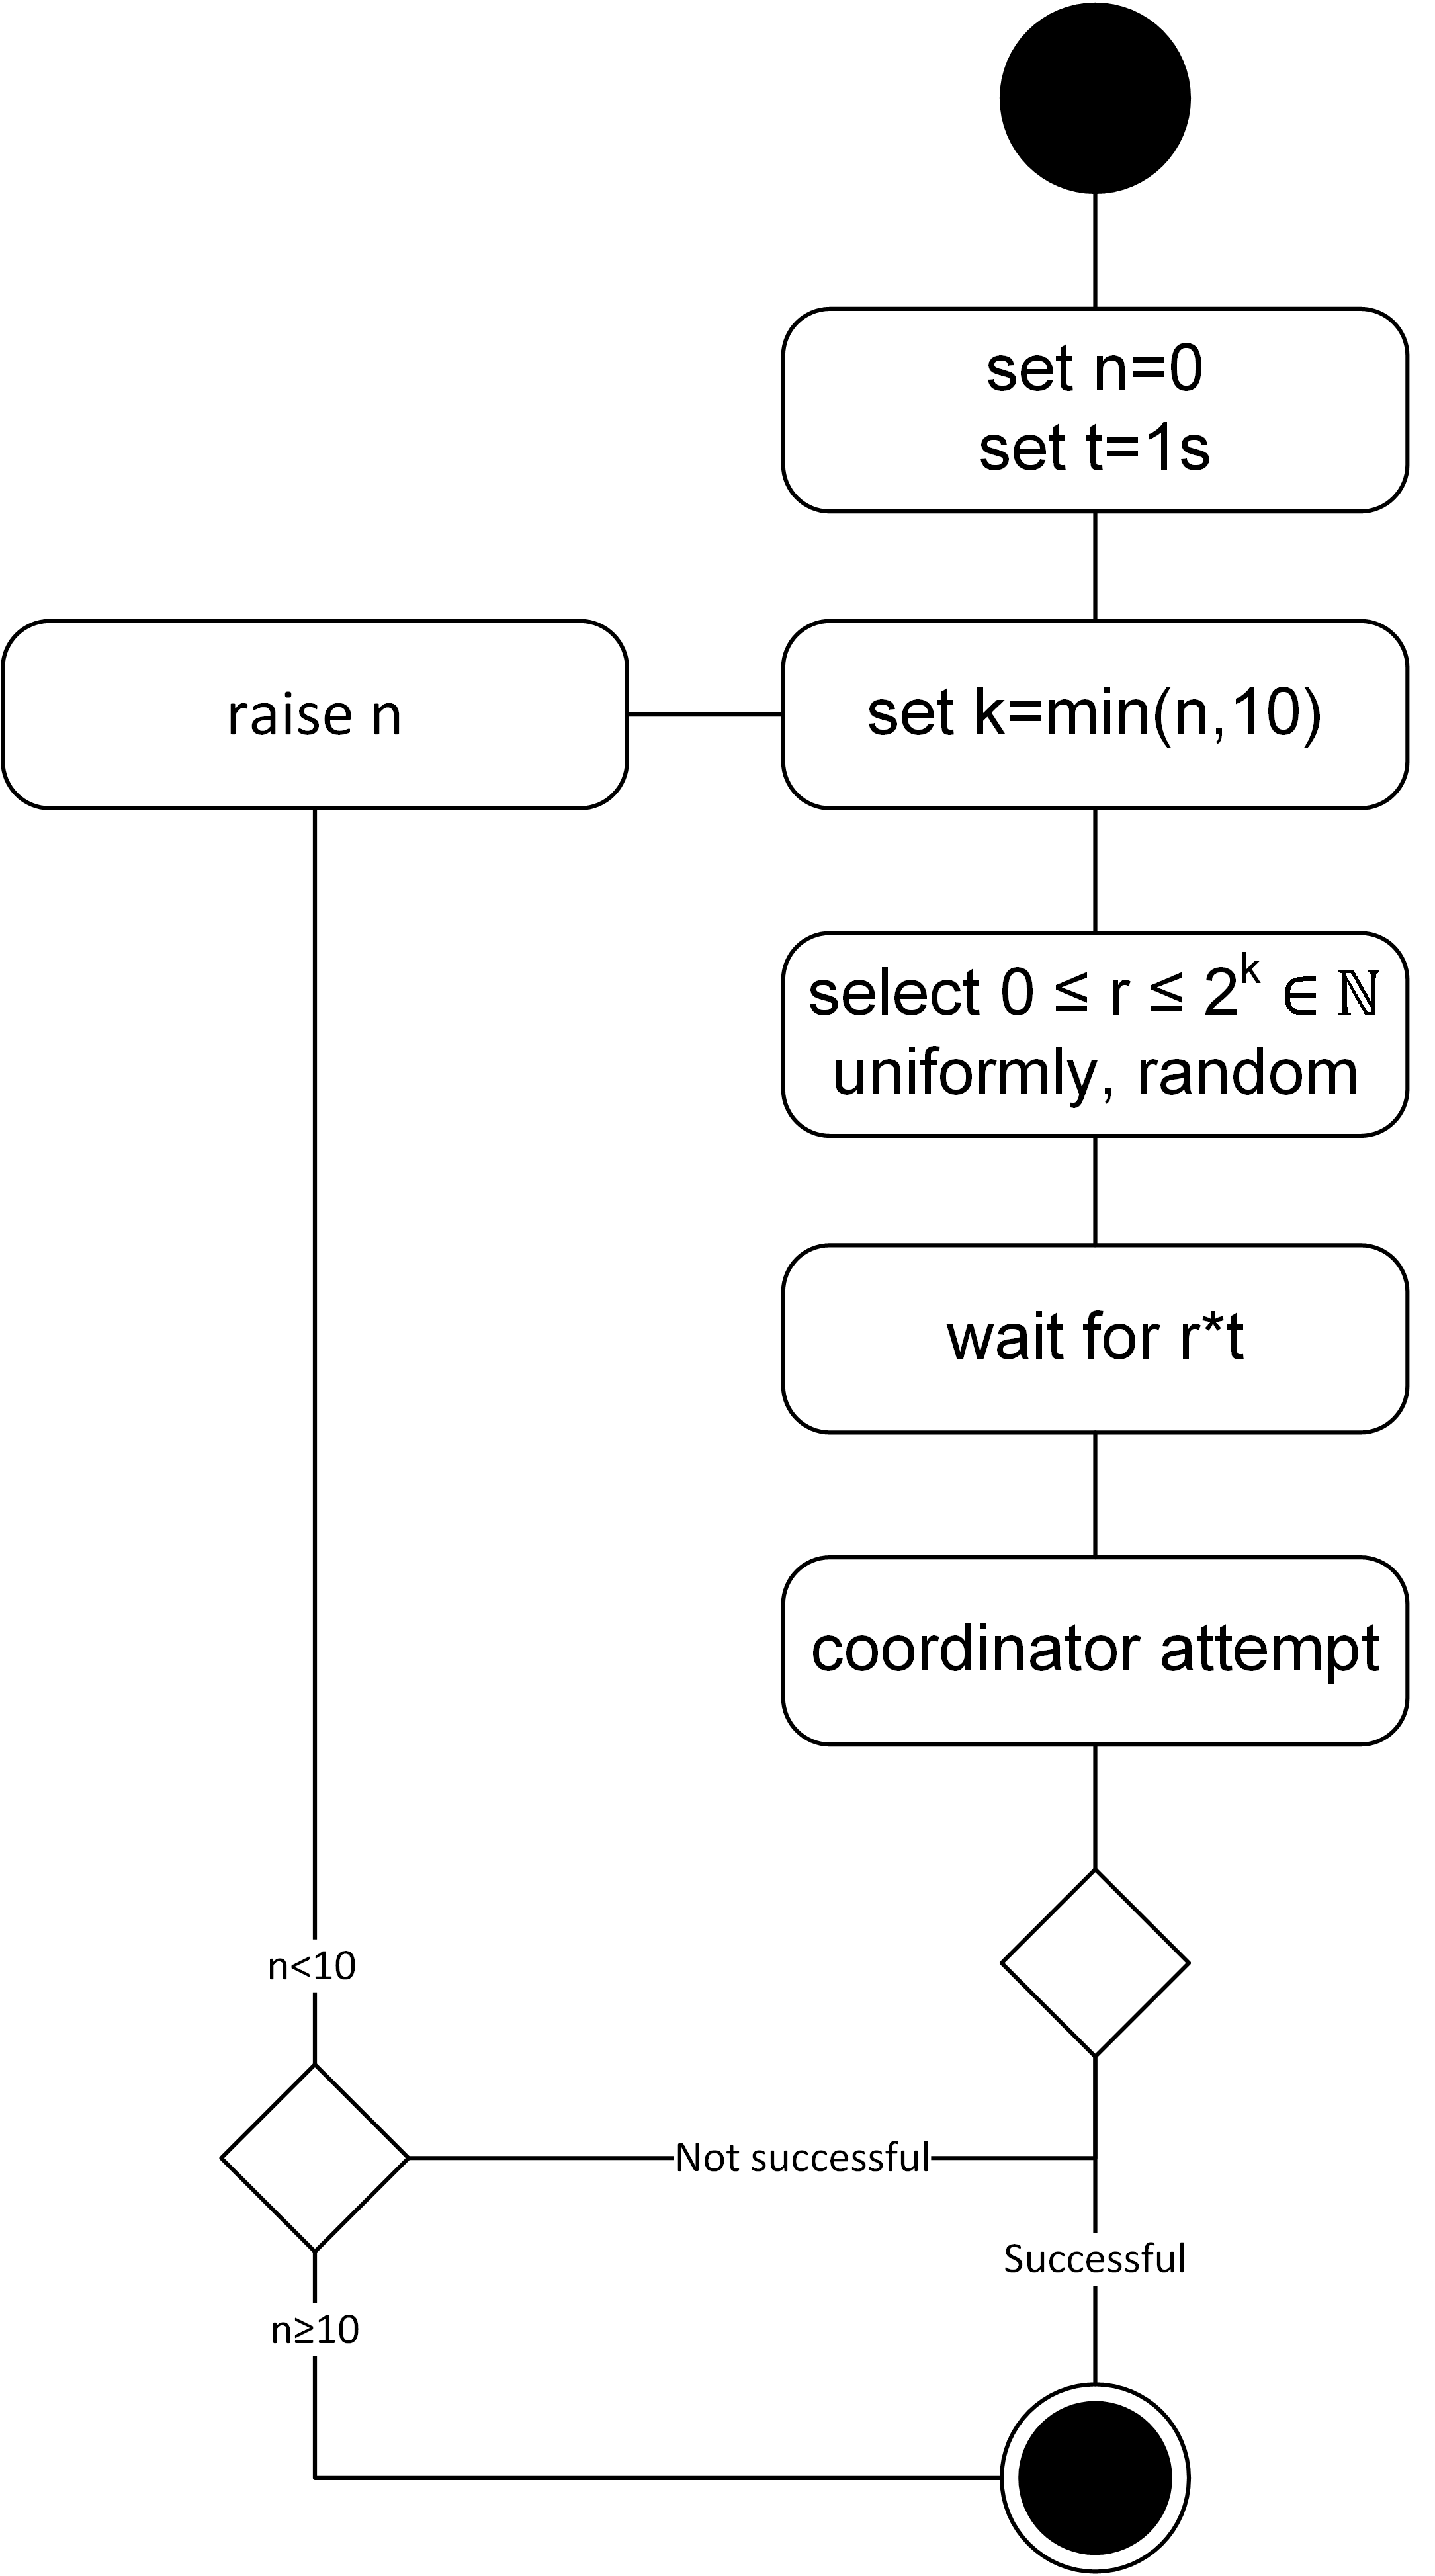
\includegraphics[scale=0.8]{figures/exponential-backoff.png}
\end{figure}

\todo*{Reduction of active connections; compare number of additional rounds needed; discuss timeouts}

In regard to the execution of the \gls{SMPC} protocols in \ref{req:SMPC Module}, the coordinator has to find a computation group. In a mesh network with routing and point-to-point encryption as displayed in \autoref{figure:Formation of fully meshed computation group - a}, the green marked coordinator can simply broadcast a computation request and responding nodes form the computation group. Caused by the technical limitations (see \autoref{practicability of an implementation}), the coordinator has to find a fully meshed group within its reach: this guarantees that each node can directly communicate with all computation partners and messages required for securing the channel are not passed through other nodes. First the coordinator $n_1$ discovers nearby nodes (see \autoref{figure:Formation of fully meshed computation group - b}). Then a list of these devices (identified by \gls{MAC} address) is sent to every neighboring node (see $n_2$ to $n_7$ in \autoref{figure:Formation of fully meshed computation group - c}). Each node responds with the intersection of the received device list with the own list of discovered devices (see \autoref{figure:Formation of fully meshed computation group - d}). To reduce the payload of the responses, they only contain a list of booleans, indication if the device with the same index in the received device list is seen by the node. The coordinator then computes the maximum group of fully meshed nodes and sends computation partners an associative array assigning new 8-bit ids (see \autoref{figure:Formation of fully meshed computation group - e}), which reduce the payload in following steps. Nearby nodes, that are not part of the computation group, receive an indicator to abort the computation. Each node in the computation group has a list of the group and the assigned ids and can exchange public keys with group members, forming a fully meshed, end-to-end encrypted group (see figure \ref{figure:Formation of fully meshed computation group - f}).

\begin{figure}[!htb] % h for placement here

	\centering
	\subfloat[Coordinator initialzation]{%
		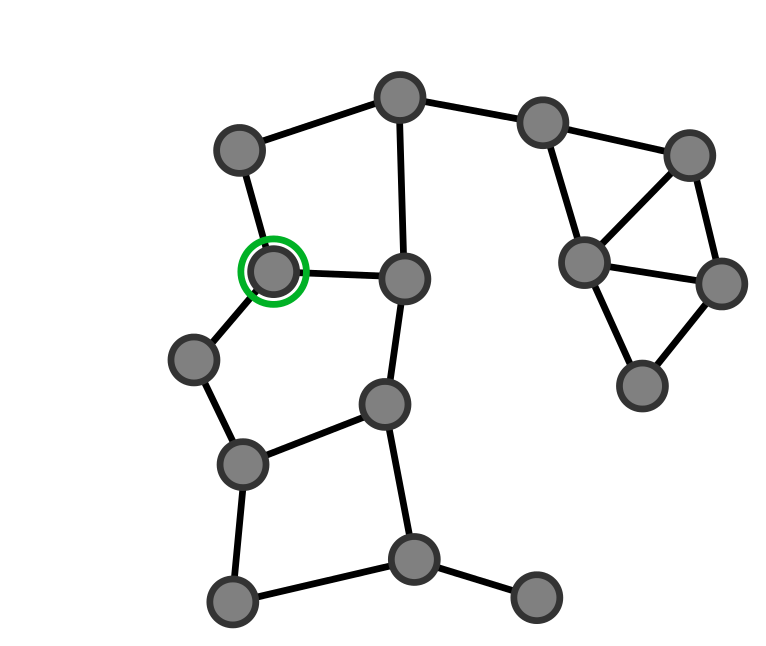
\includegraphics[scale=1.0]{figures/coordinator-1.png}
		\label{figure:Formation of fully meshed computation group - a}
	}%
	\hfill
	\subfloat[Coordinator discovery]{%
		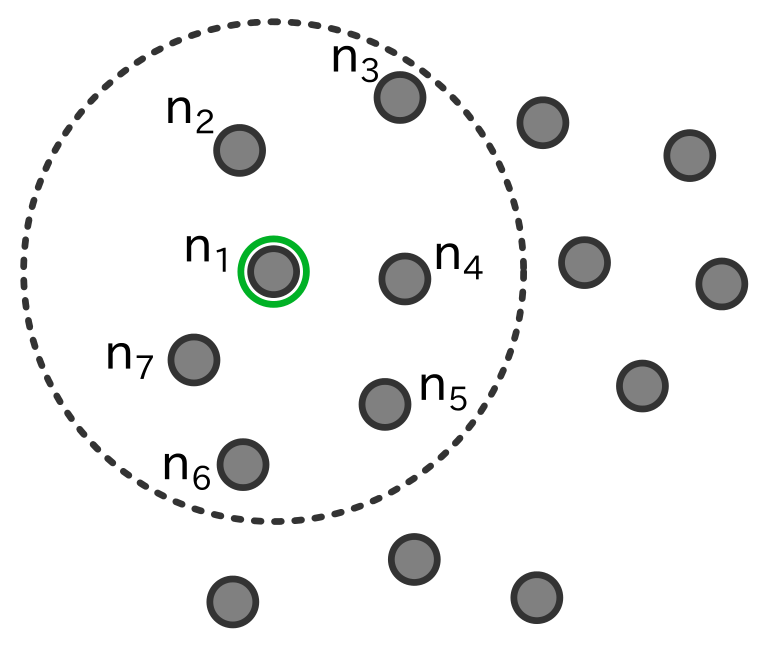
\includegraphics[scale=1.0]{figures/coordinator-2.png}
		\label{figure:Formation of fully meshed computation group - b}
	}\\
	\subfloat[Coordinator sends discovery request and own node list]{%
		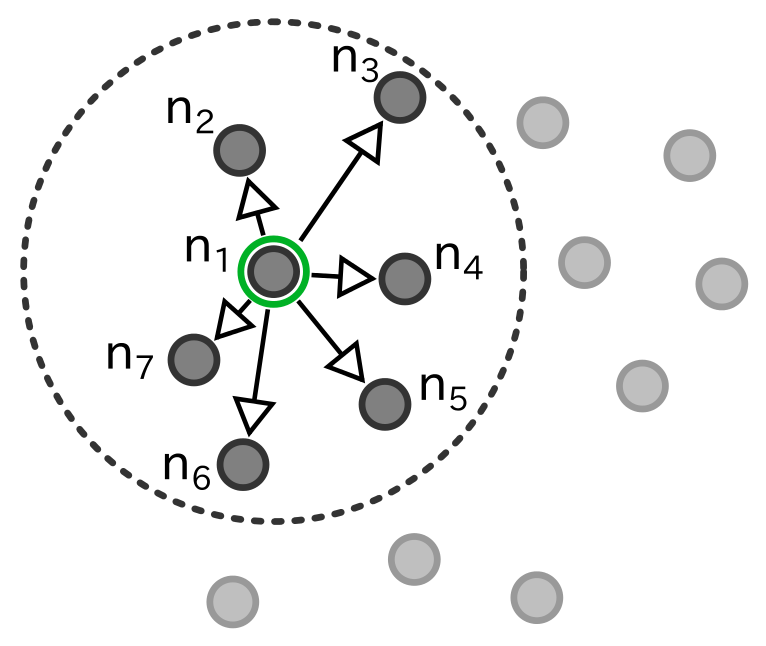
\includegraphics[scale=1.0]{figures/coordinator-3.png}
		\label{figure:Formation of fully meshed computation group - c}
	}%
	\hfill
	\subfloat[Nodes respond with intersection of discovered devices]{%
		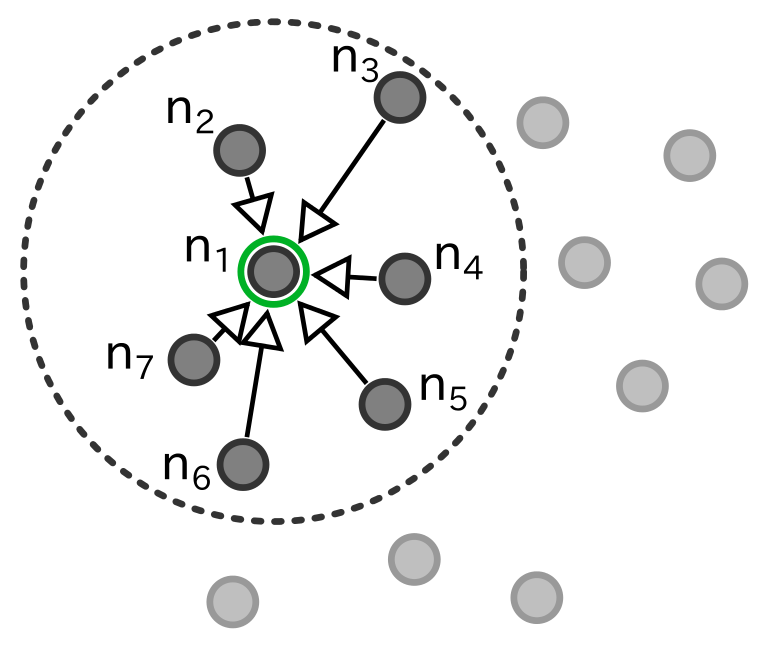
\includegraphics[scale=1.0]{figures/coordinator-4.png}
		\label{figure:Formation of fully meshed computation group - d}
	}\\
	\subfloat[Coordinator computes and announces fully meshed computation group]{%
		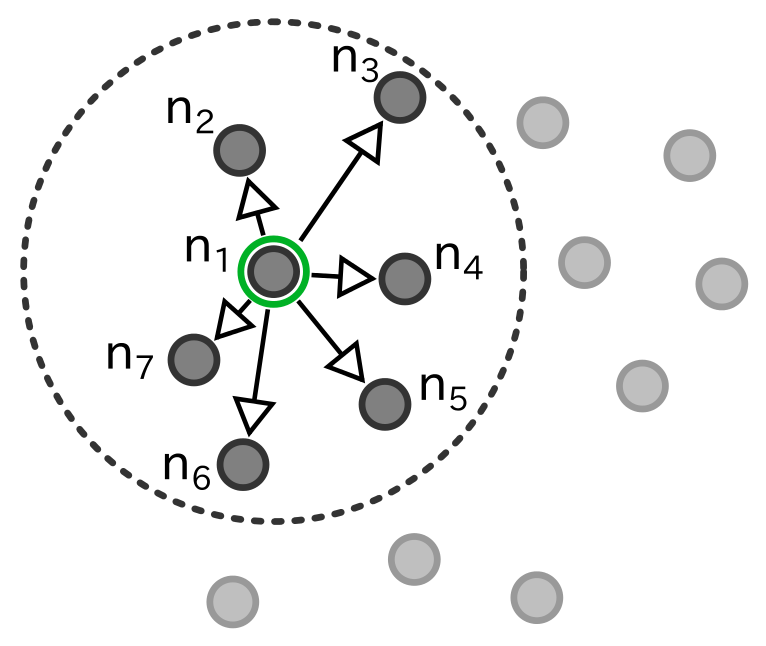
\includegraphics[scale=1.0]{figures/coordinator-5.png}
		\label{figure:Formation of fully meshed computation group - e}
	}%
	\hfill
	\subfloat[Meshed network is ready for \gls{SMPC} computation]{%
		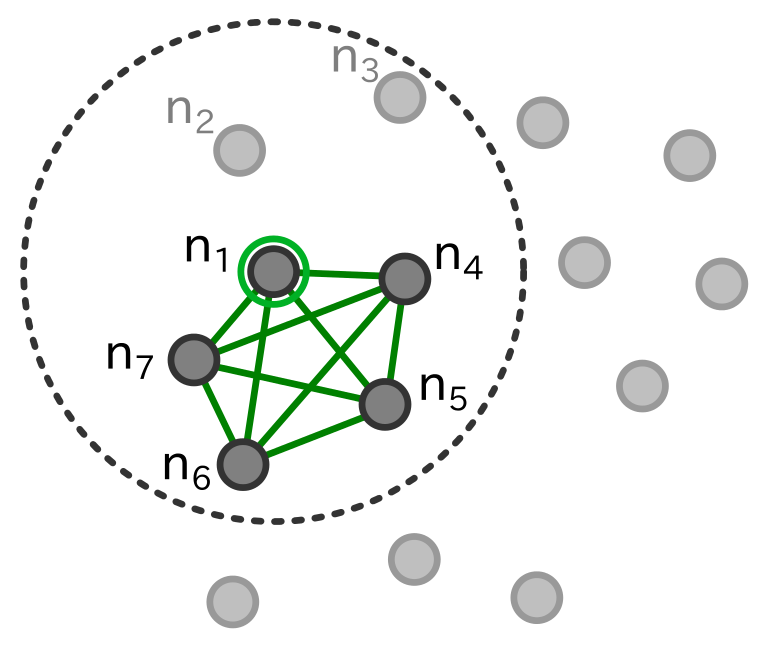
\includegraphics[scale=1.0]{figures/coordinator-6.png}
		\label{figure:Formation of fully meshed computation group - f}
	\caption{Formation of fully meshed computation group} \label{figure:Formation of fully meshed computation group}
	}
\end{figure}

Since parallel message exchange for the computation group cannot be guaranteed (see \autoref{practicability of an implementation}), the coordinator controls sequential message exchanges with token passing in accordance with \ref{req:Token-Passing}. For example when $n$ nodes want to exchange $n$ secrets divided into $n$ shares each, the coordinator first requests successively the shares for himself ($s_i,1$) from the other $n-1$ nodes, while transmitting his own shares ($s_1,j$) with the request. Then the communication token gets passed to the next node, which in turn requests the shares for himself from the other $n-2$ nodes while transmitting his own shares and so on. An exemplary share-exchange for $n=3$ with token-passing is illustrated in figure \ref{figure:coordinator token passing}.

\begin{figure}[!htb] % h for placement here
	\caption{\gls{UML} sequence diagram for passing of communication token t} \label{figure:coordinator token passing}
	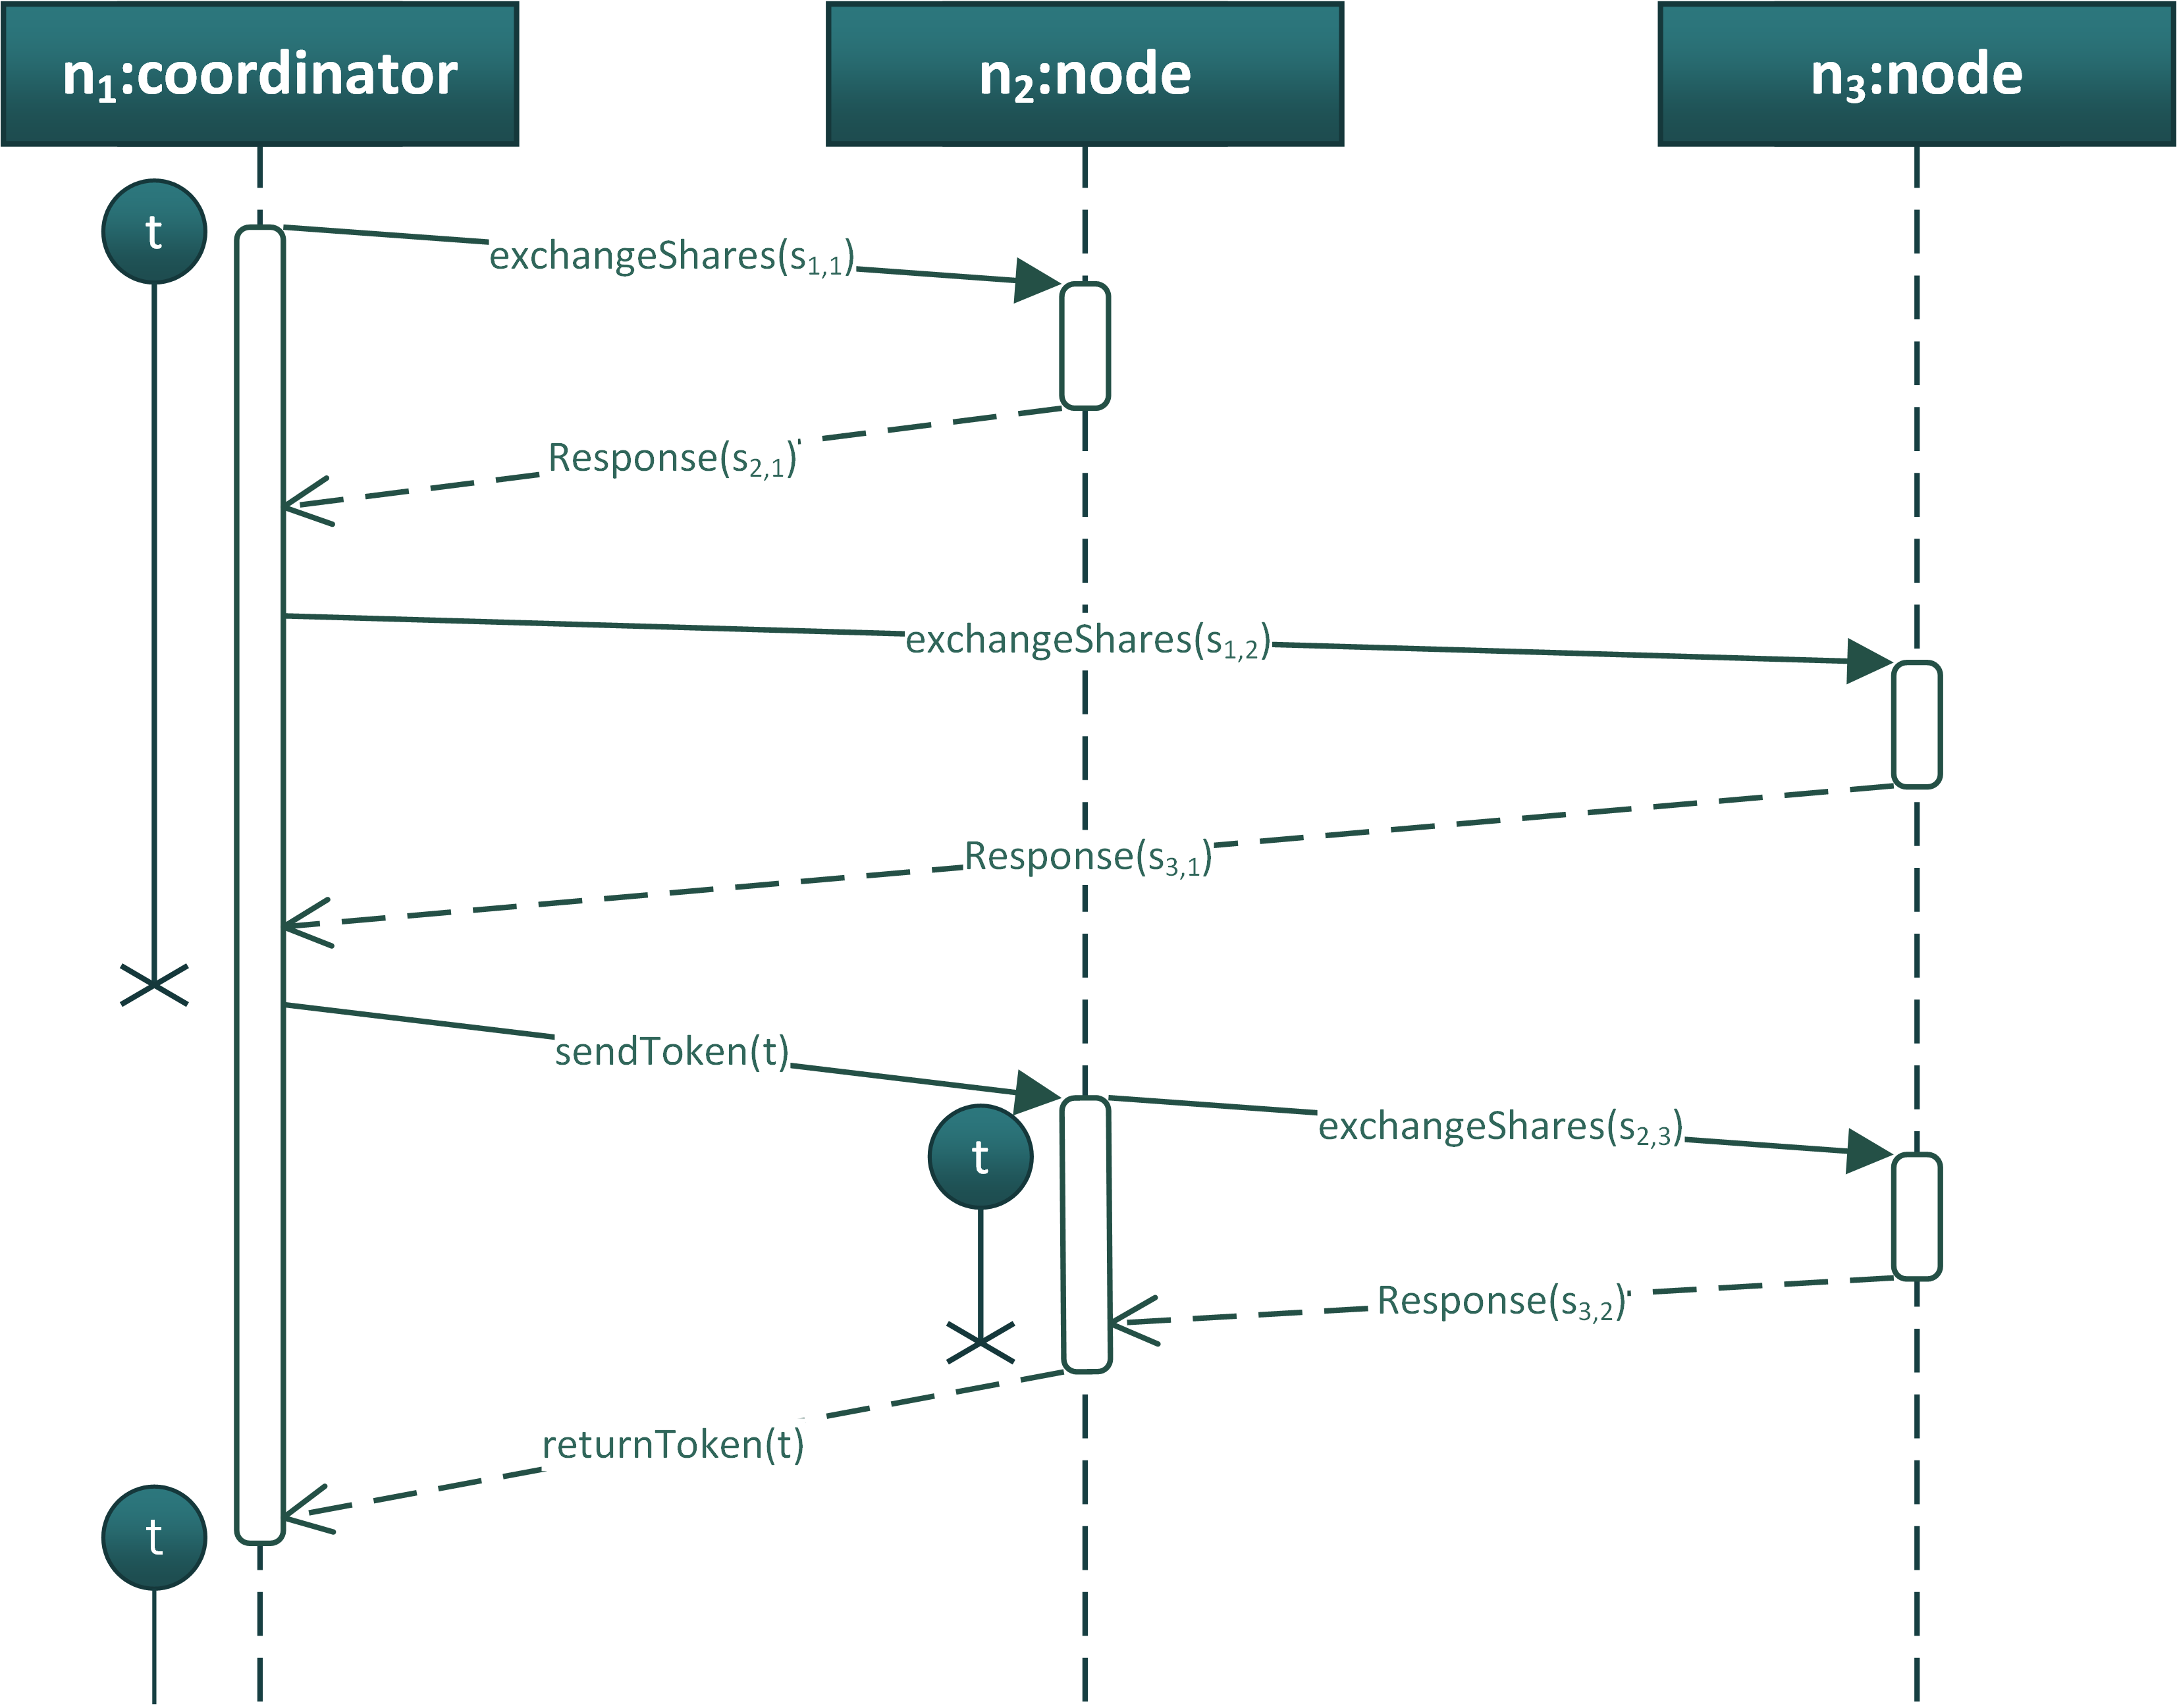
\includegraphics[scale=1.0]{figures/token-passing-ion.png}
\end{figure}

The combination of processes with the same communication partners, single-digit bytes of payloads and short process termination is a good option to reduces the total message-occurrence in the network: for example when a coordinator requests the states of nearby nodes, it can be combined with the clock synchronization.

\subsection{Clock Synchronization} \label{Clock synchronization}

For statistical data in a gamification system, the sequence of events in infinitesimal time units is not as important as comparing the data for the same durations in \gls{UTC}, so a synchronization of physical clocks is needed as requested in \ref{req:Clock Synchronization}. In this thesis  the well known Berkeley-algorithm for internal clock synchronization in distributed systems is used as described in \textcite{Ghosh2015}.

\noindent The coordinator
%\vspace{-\topsep}
\begin{enumerate}
	%\itemsep-0.5em
	\item requests the current time values $t_i$ from participating nearby nodes $i$.
	\item computes the average of these values $t_{average}$.
	\item reports back the adjustments $\Delta_{i}=t_{average}-t_i$
\end{enumerate}

Since the communication between the coordinator and a node takes time, the received response is already outdated. This is compensated by observing the \gls{RTT} and using half of the duration as a correction value (compare \ref{eq:berkeley RTT}). The \gls{RTT} is herein the timespan between sending a request to a node and receiving its response (see figure \ref{figure:berkeley RTT}).
\begin{alignat}{1}
t'_i &=t_i+\underbrace{\frac{RTT}{2}}_{\text{correction value}}=t_i+\frac{t_e-t_s}{2} \label{eq:berkeley RTT}
\end{alignat}

%\begin{figure}[!htbp] % h for placement here
%	\caption{Round Trip Time} \label{figure:berkeley RTT}
%	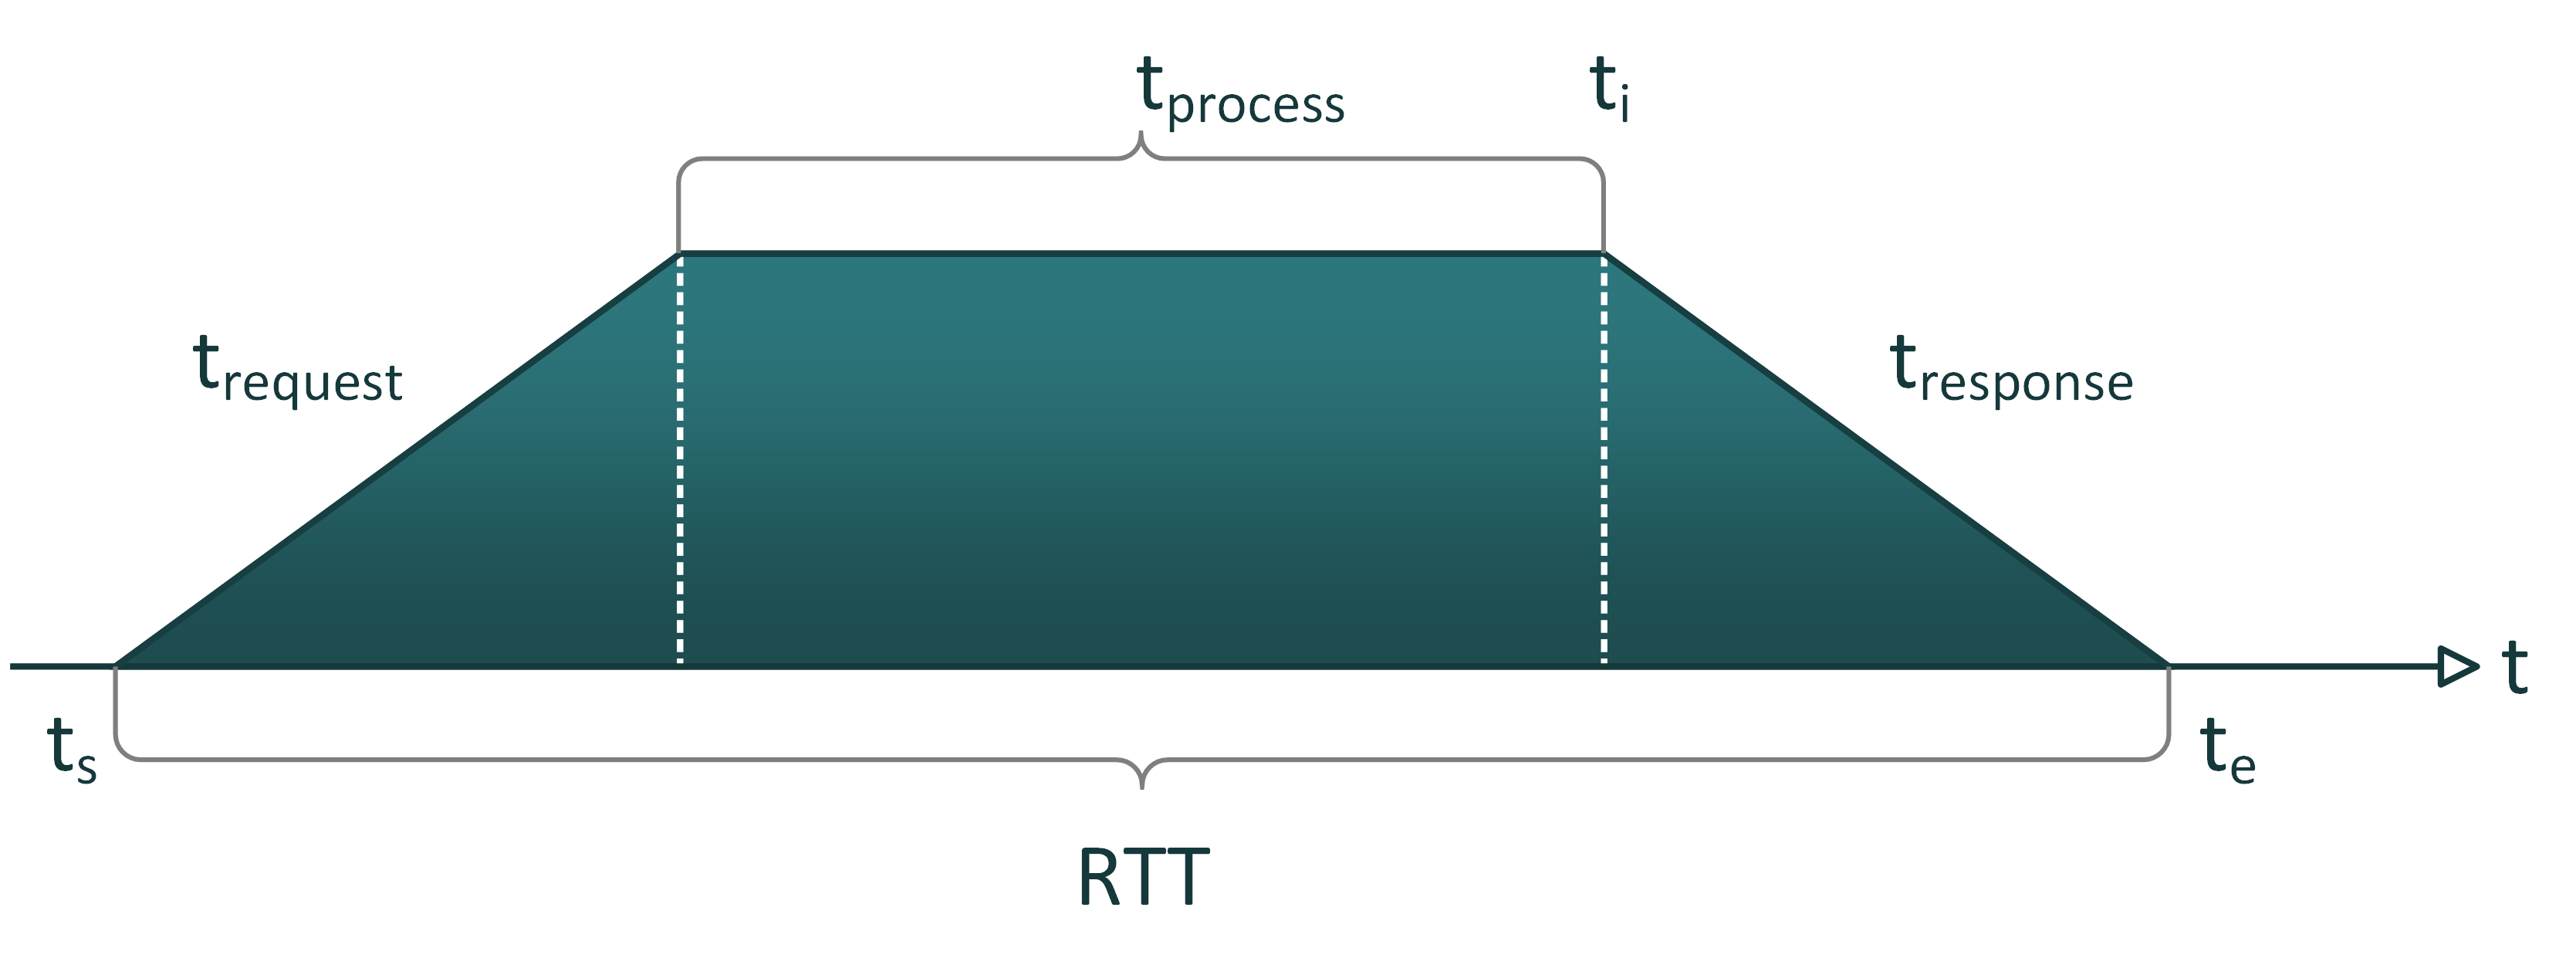
\includegraphics[scale=1.0]{figures/berkeley-ion.png}
%\end{figure}

By sending the adjustments $\Delta_i$ instead of the adjusted time, the receiving nodes do not need to compensate the received value with the \gls{RTT}. Figure \ref{figure:berkeley example} depicts the computation of the adjustments using Berkeley with \gls{RTT} correction for three nodes. 

%\begin{figure}[!htbp] % h for placement here
%	\caption{Example computation of adjustments with Berkeley} \label{figure:berkeley example}
%	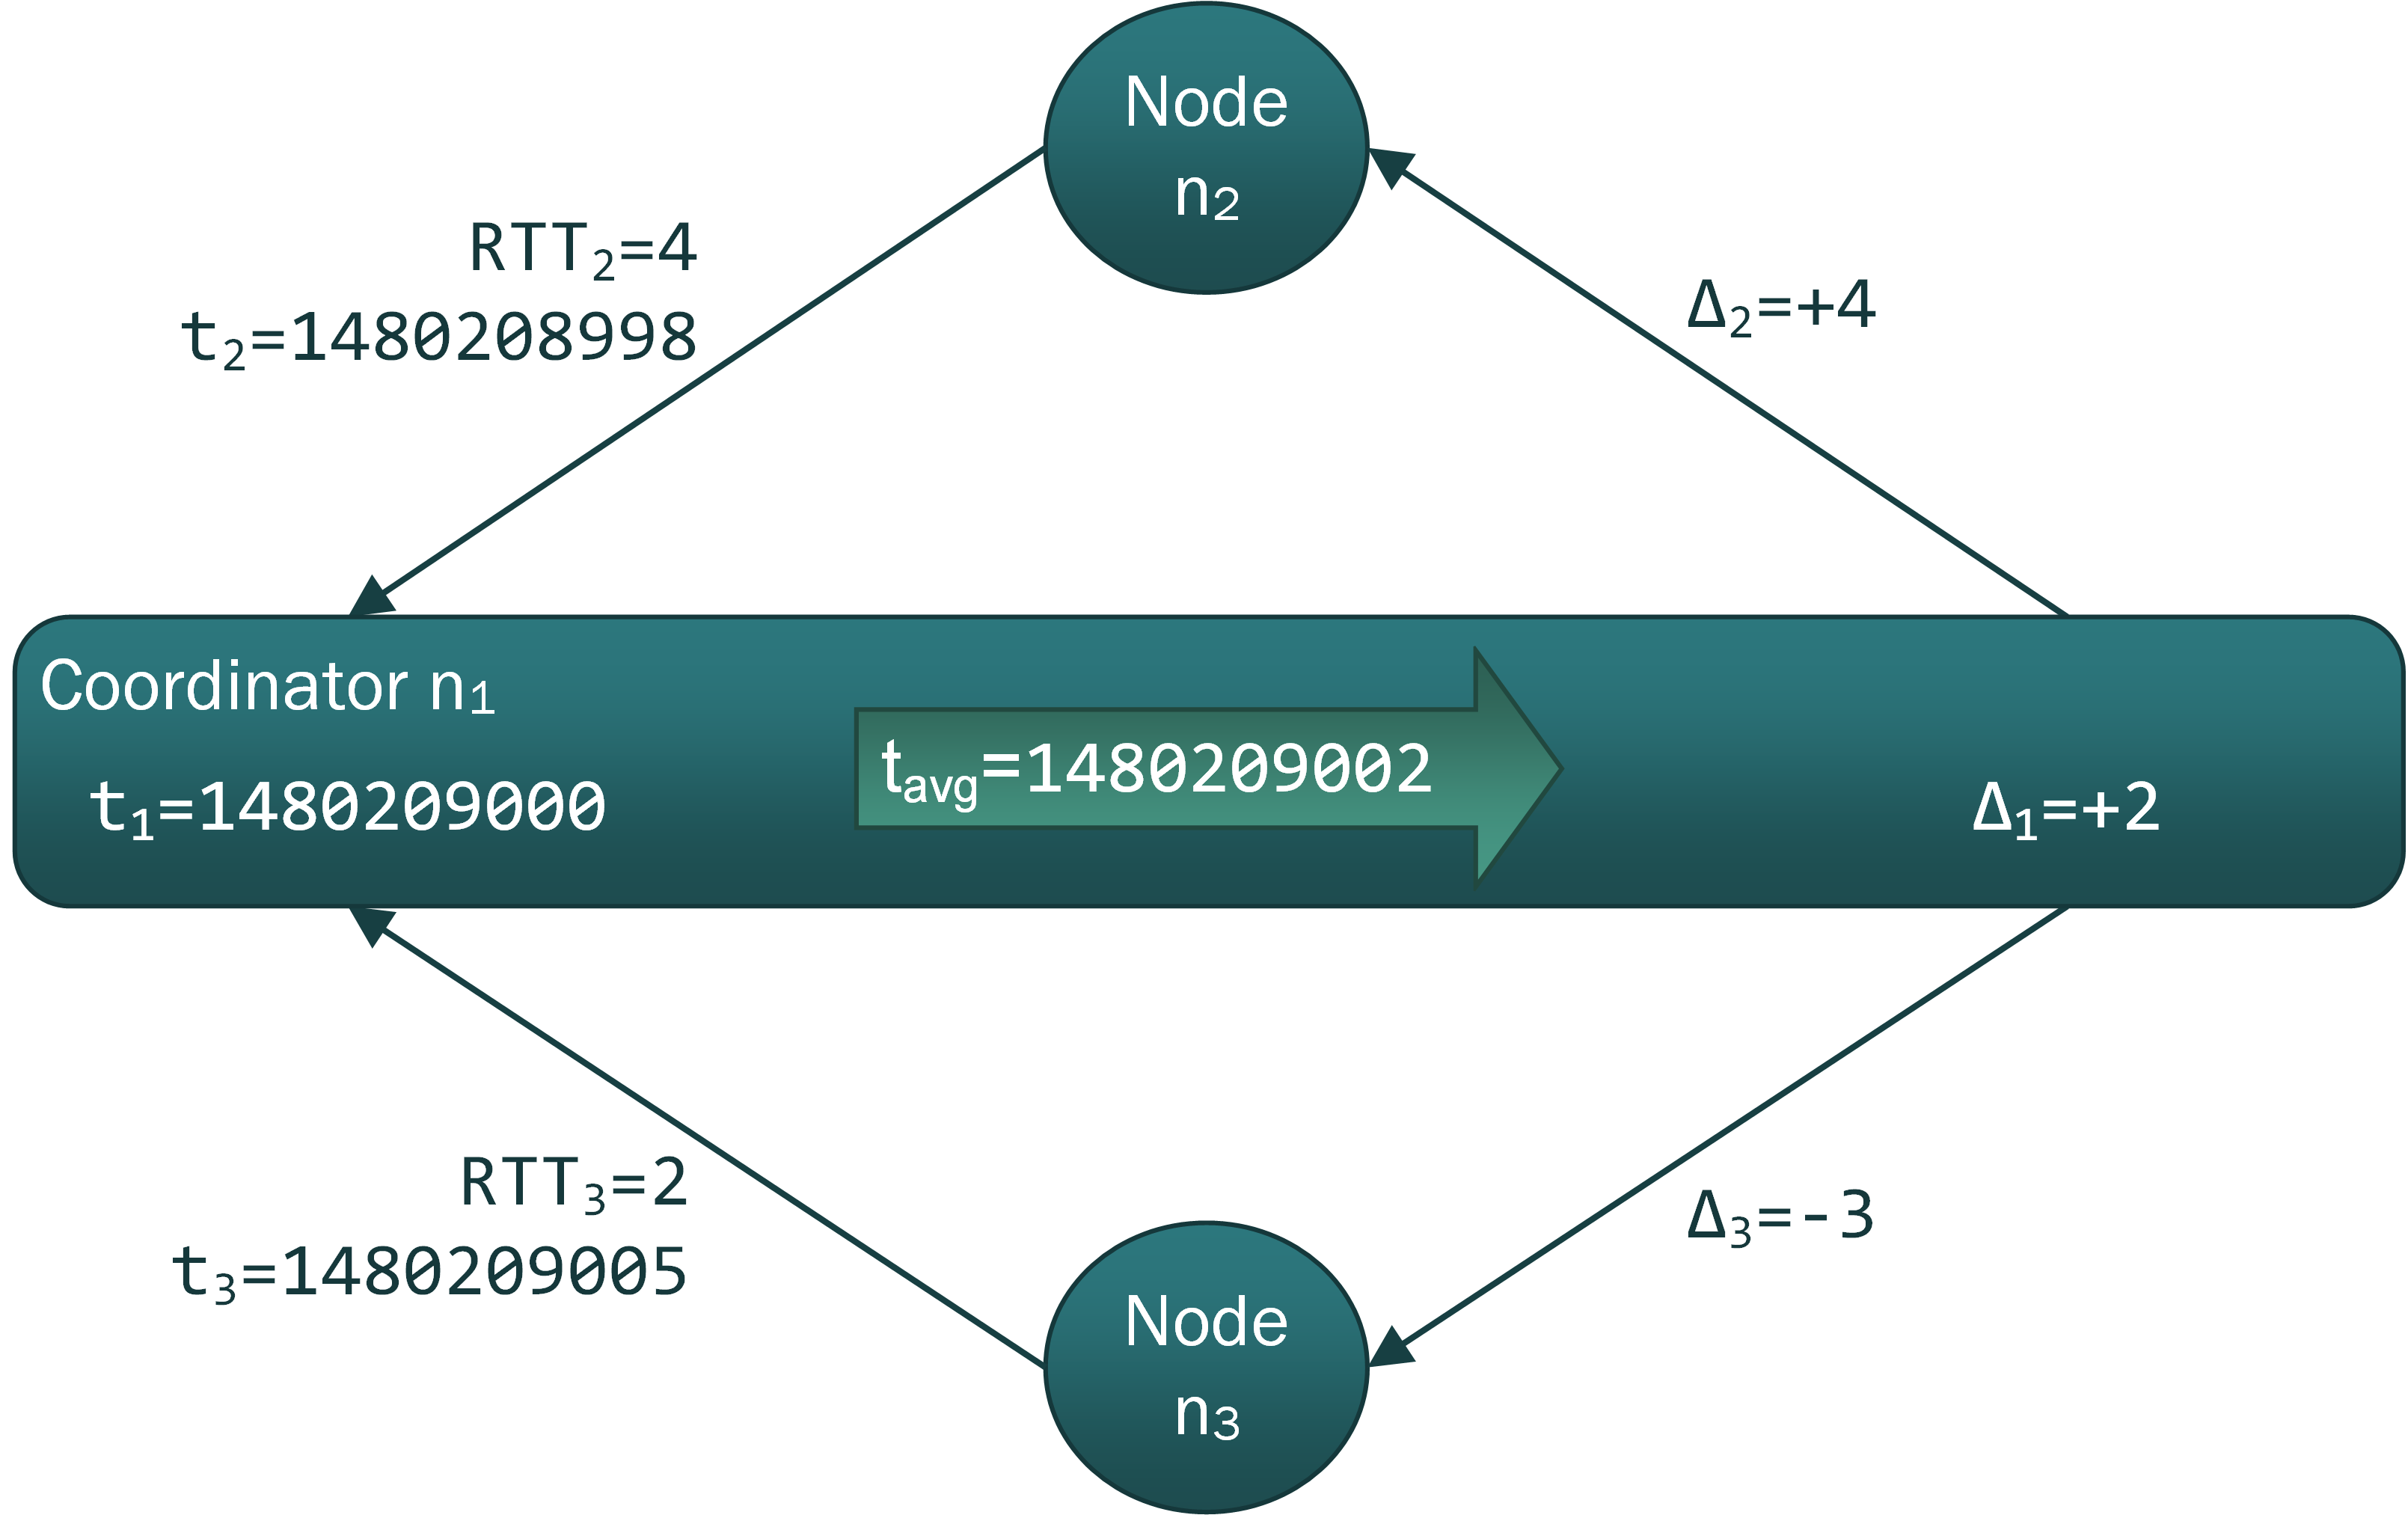
\includegraphics[scale=1.0]{figures/berkeley-example-ion.png}
%\end{figure}

\begin{figure}[!htb] % h for placement here
	\centering
	\subfloat[Round Trip Time]{%
		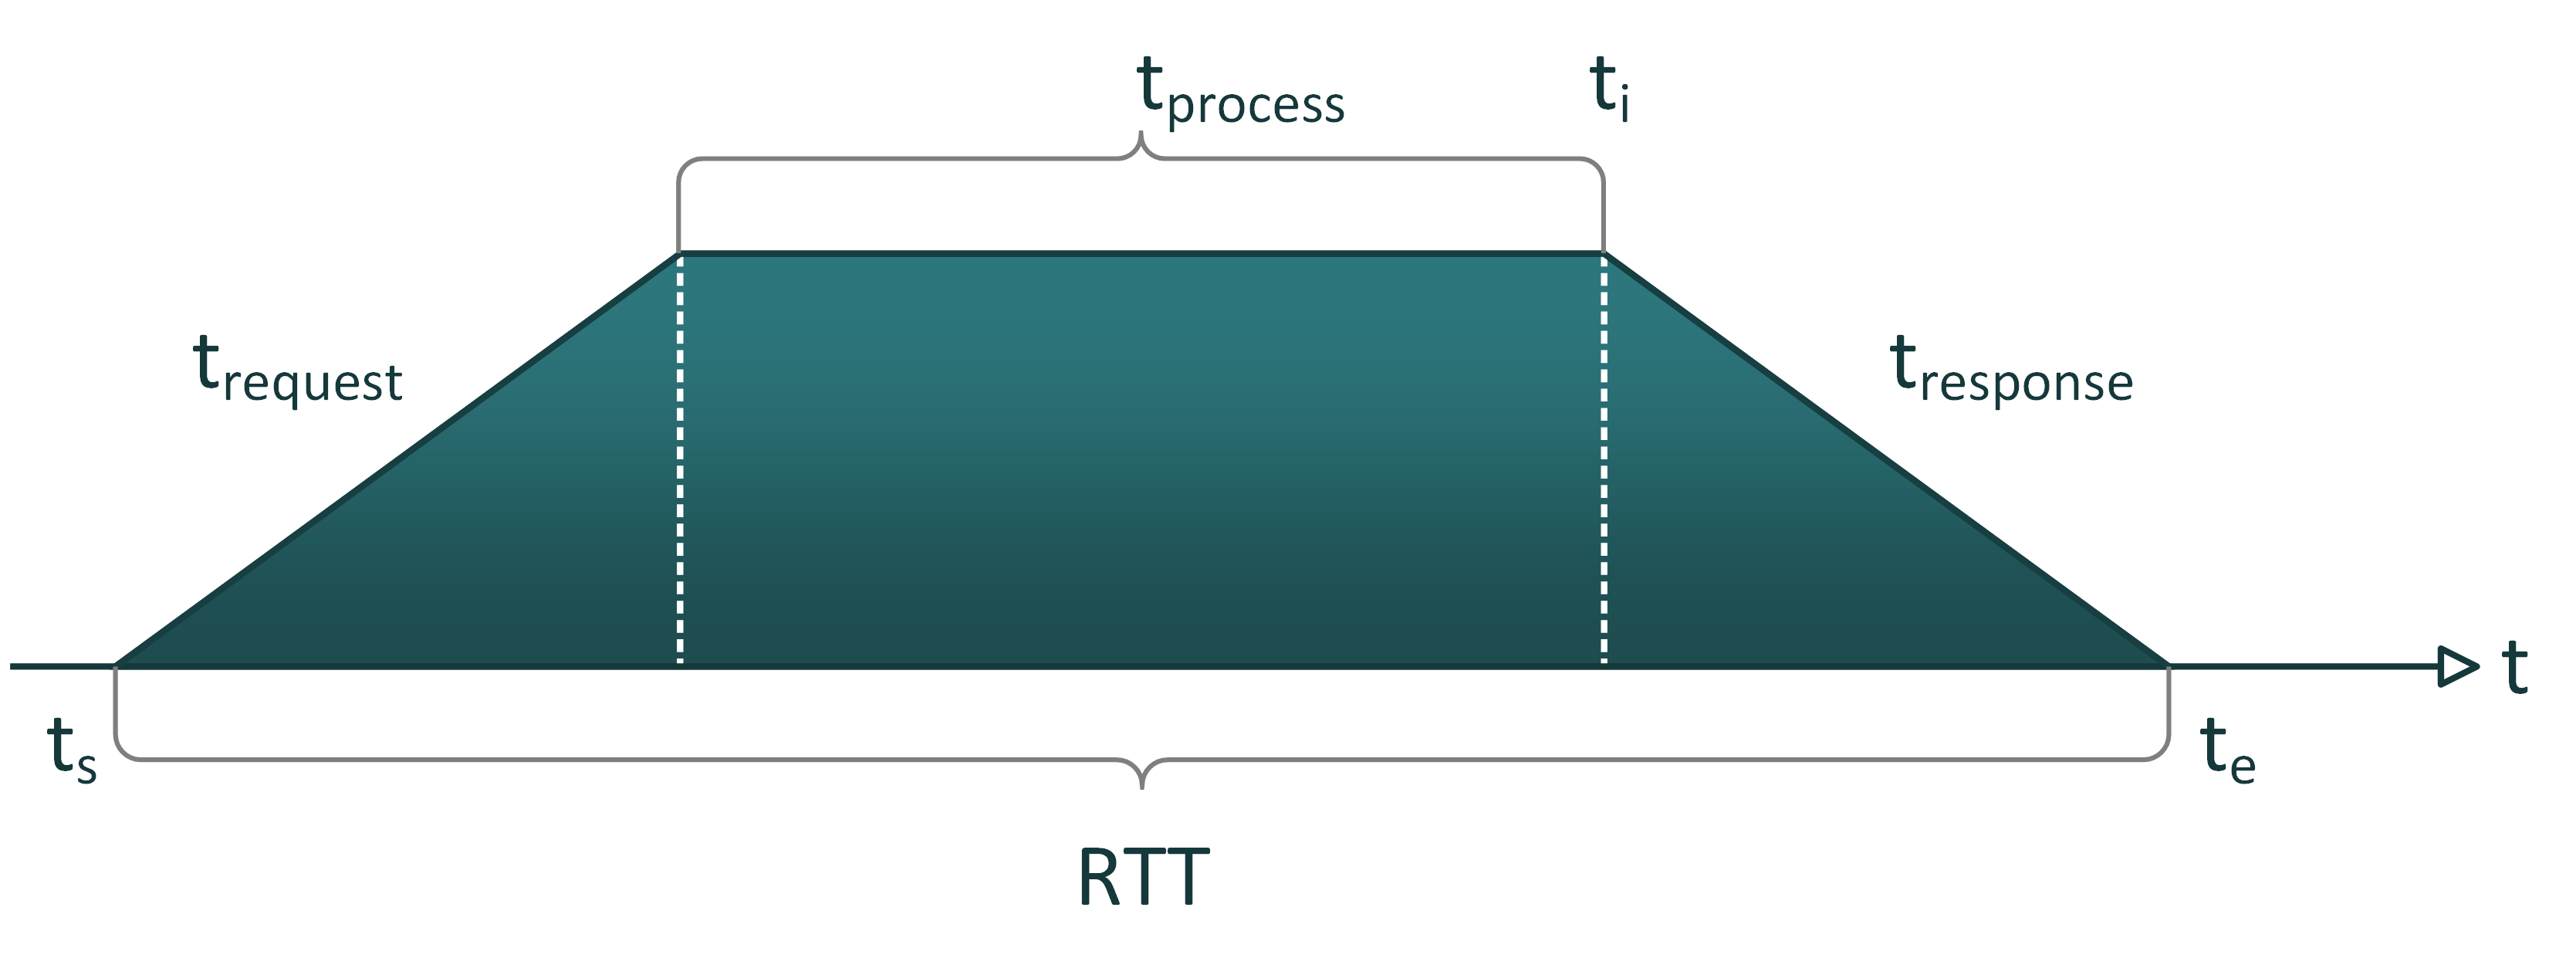
\includegraphics[scale=1.0]{figures/berkeley-ion.png}
		\label{figure:berkeley RTT}
	}%
	\\
	\subfloat[Example computation of adjustments with Berkeley]{%
		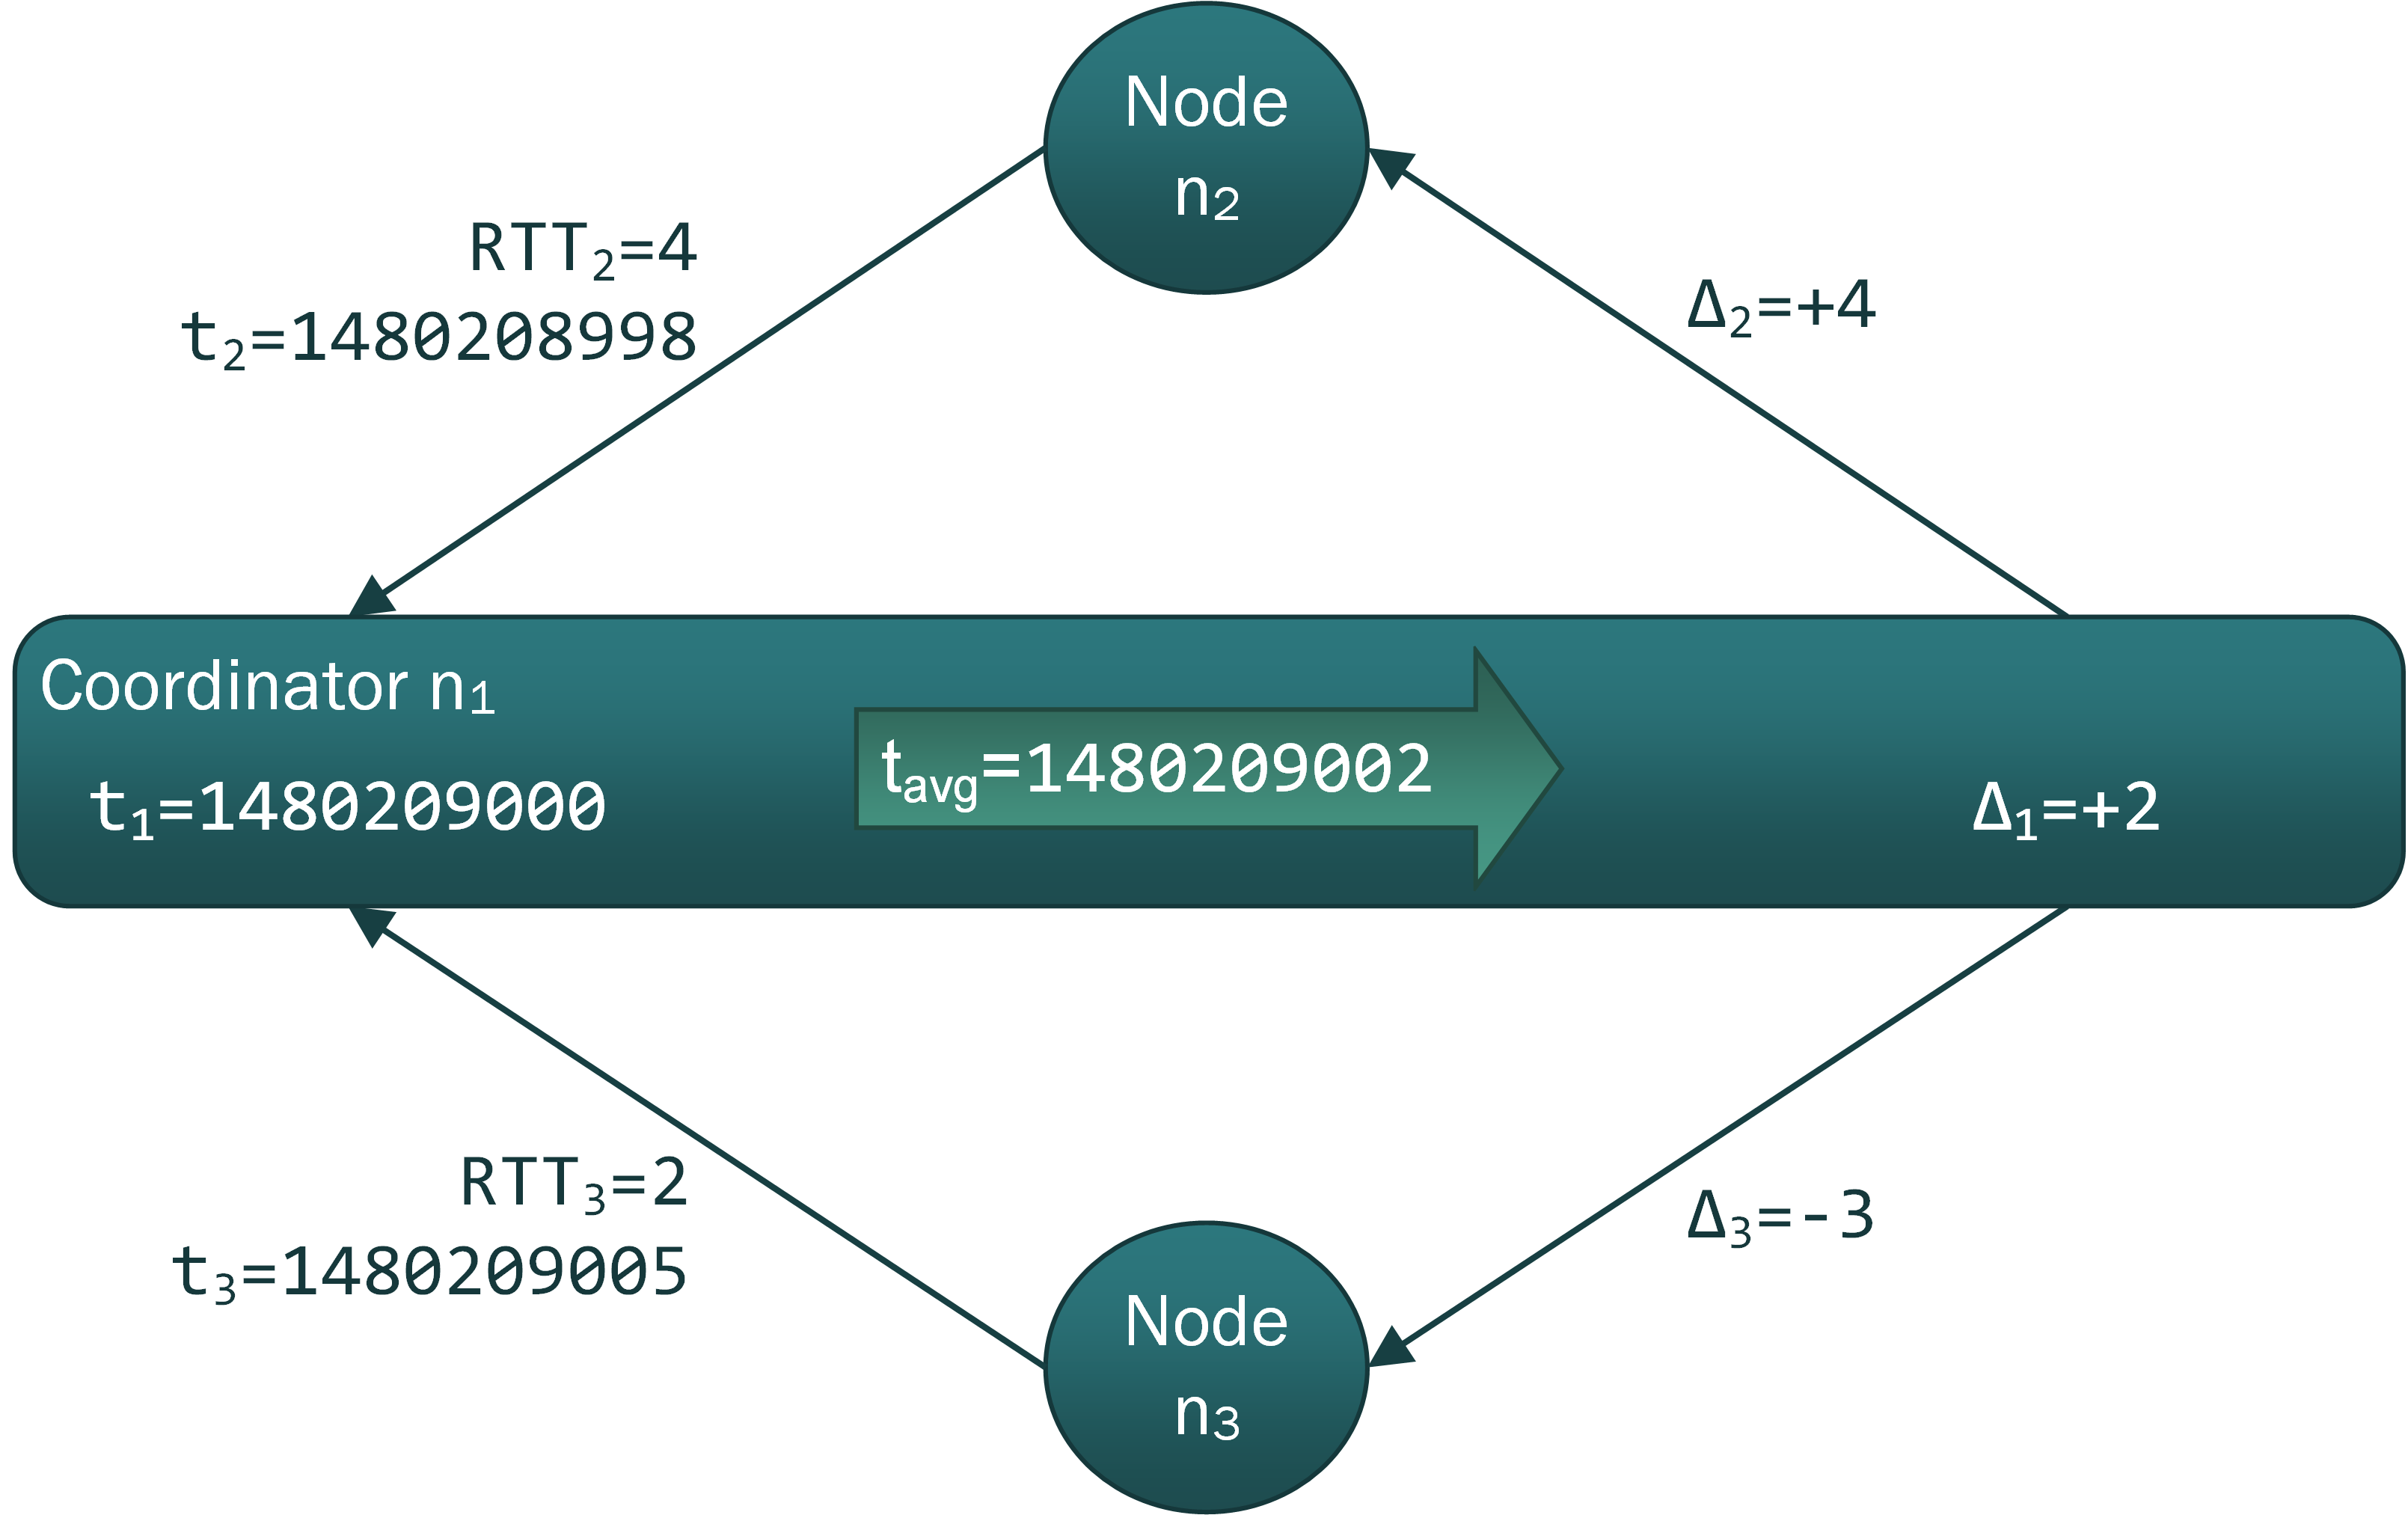
\includegraphics[scale=0.8]{figures/berkeley-example-ion.png}
		\label{figure:berkeley example}
	}
	\caption[Distributed clock synchronzation]{Internal clock synchronzation in distributed networks} \label{figure:Distributed clock synchronzation}
\end{figure}

For further improvement of the accuracy the processing duration between receiving a request and sending the response $t_{process}$ can be measured and send to the coordinator. In this thesis the simple approximation for $t_{response}$ is used, since the additional payload extends the transmission duration. The \gls{RTT} has to be below an upper bound though, otherwise there is to much uncertainty regarding the influence of $t_{request}$, $t_{process}$ and $t_{response}$.
Also bounds for the deviation of the time can be defined to reduce the influence of outliers.

The framework does not change the actual clock setting on the hosting system, but stores the computed time difference $\Delta_t$ and applies the value to all time-related actions. To make sure that a node is time-synchronized before scores and computations are acquired, it is reasonable to trigger a synchronization when the node joins the network. 

\subsection{Non-termination Detection} \label{Non-termination Detection}

Especially since the coordinator gives temporarily away the message token and goes into a waiting state, there has to be a protocol to detect non-termination for processes. Meeting \ref{req:Non-termination Detection} each request to another node and each local computation initializes the start of timers. The local timer triggers the transmission of a heartbeat message (compare \ref{req:Heartbeat}) to the coordinator, signaling that the process is still intact, but not yet finished. If the coordinator receives a heartbeat message, it informs the other nodes in the computation group (causing them to reset their local timers), and resets its local timeout-timer. If the coordinator reaches a limit for the timer without receiving a heartbeat message, non-termination is assumed and all group members are informed, that the computation failed. The heartbeat protocol for the coordinator waiting for response is outlined in figure \ref{figure:heartbeat coordinator}, while the protocol for a node in possession of the message token is displayed in figure \ref{figure:heartbeat node}.  

\begin{figure}[!htb] % h for placement here
	\centering
	\subfloat[]{%
		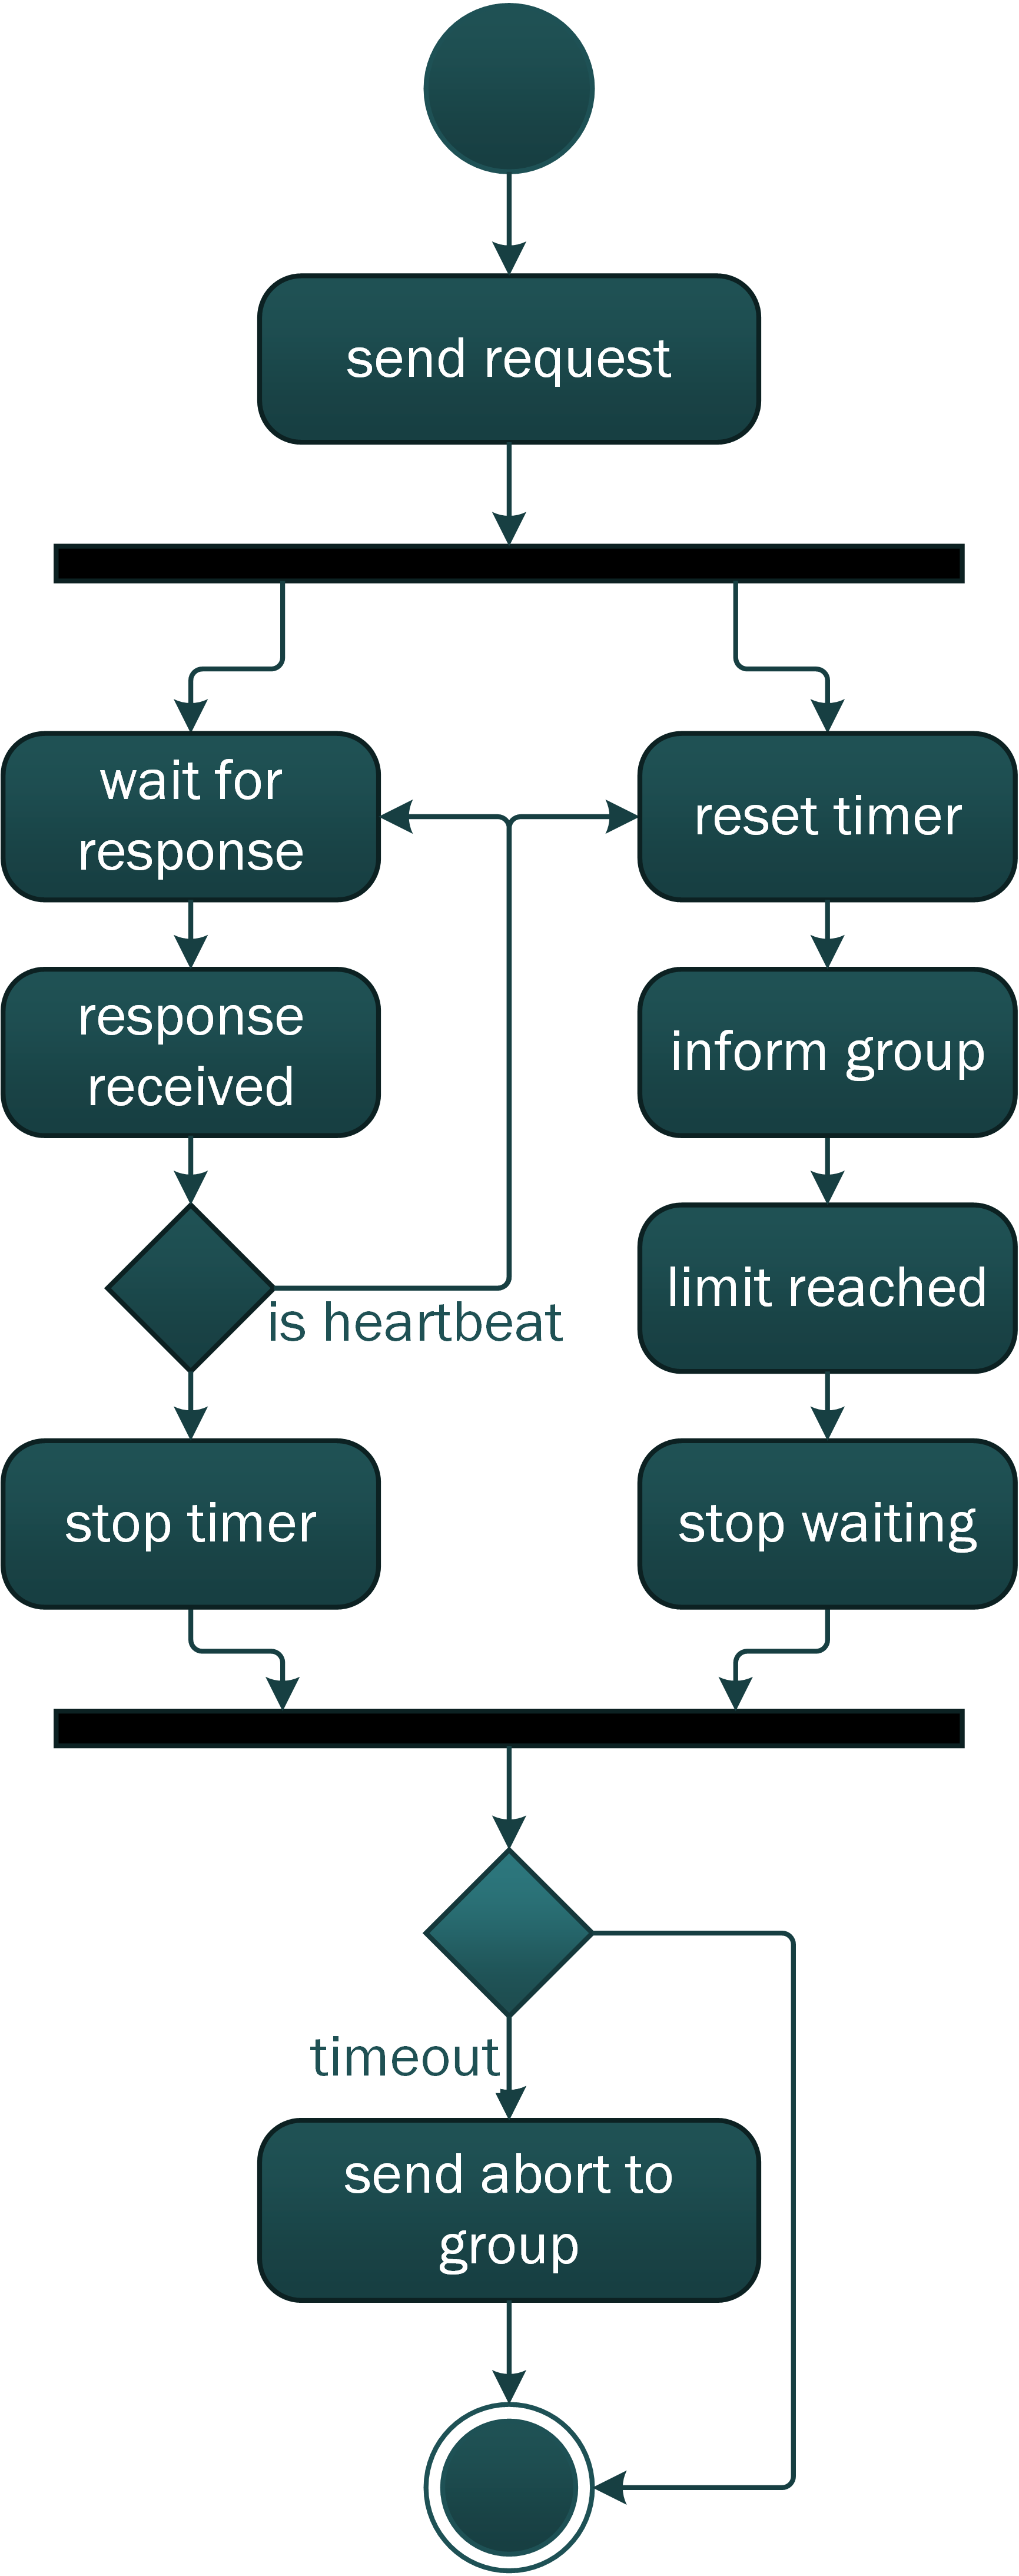
\includegraphics[scale=0.8]{figures/heartbeat-coordinator.png}
		\label{figure:heartbeat coordinator}
	}%
	\hfill
	\subfloat[]{%
		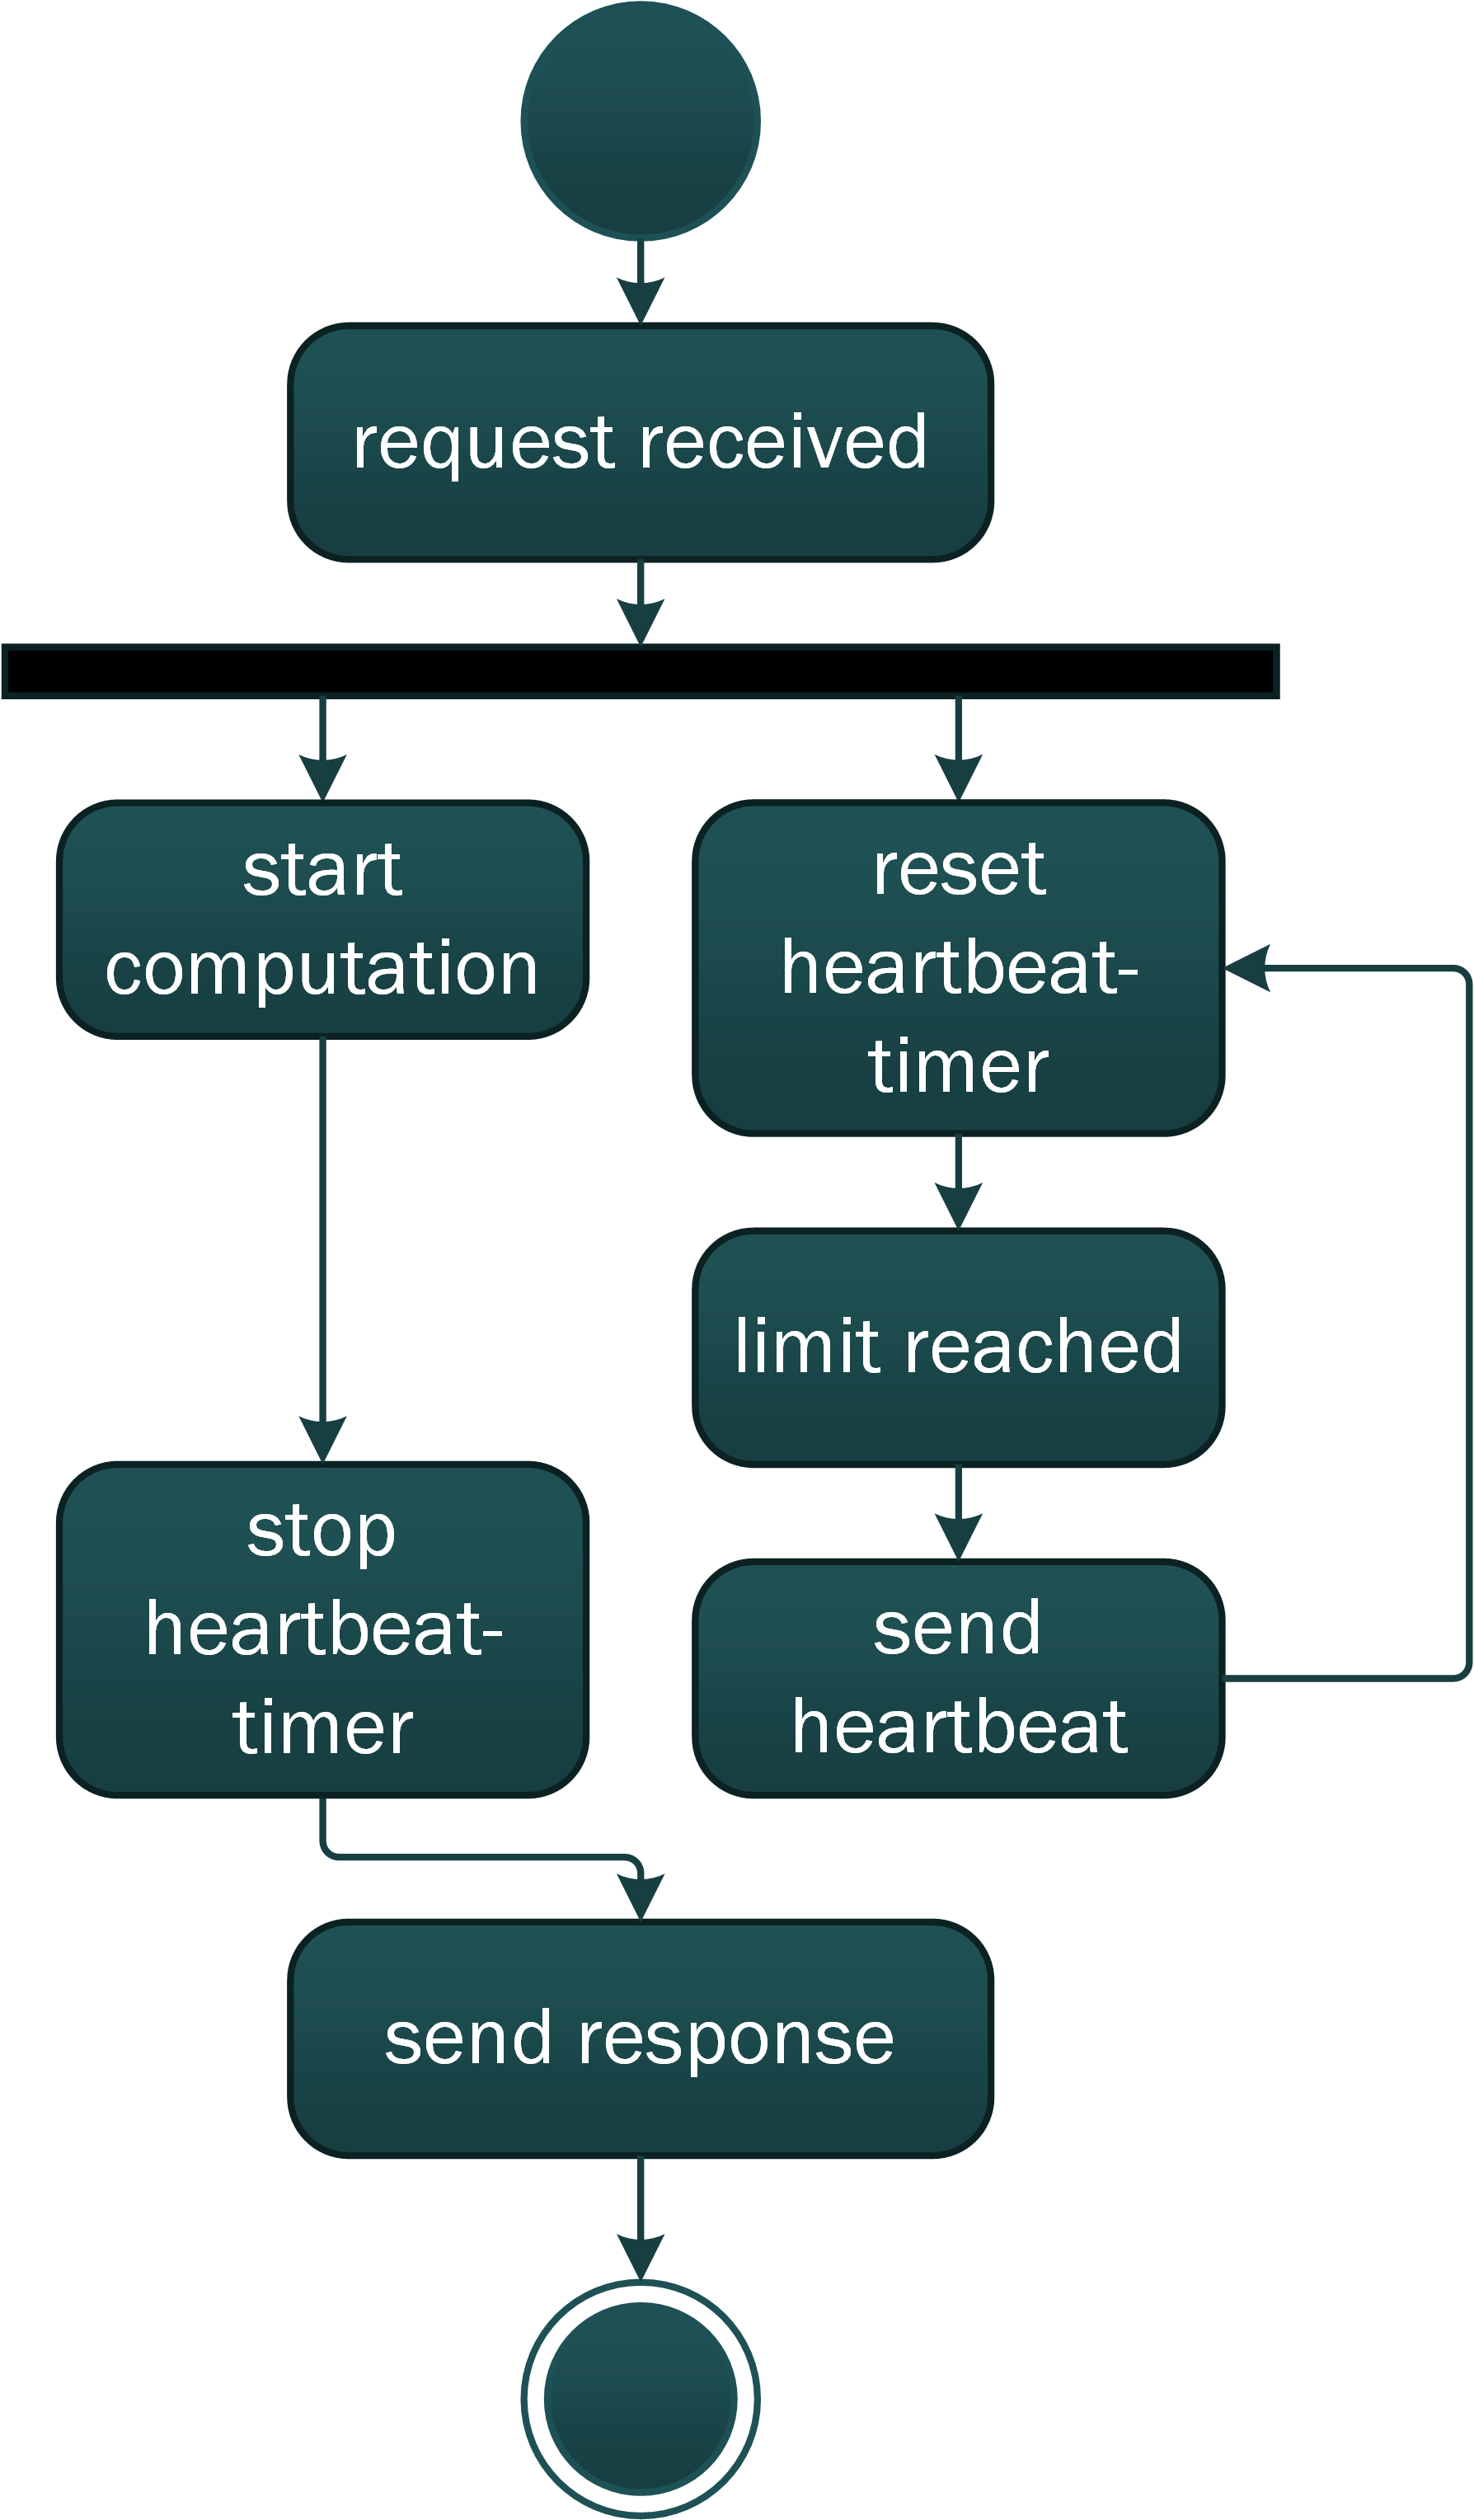
\includegraphics[scale=0.8]{figures/heartbeat-node.png}
		\label{figure:heartbeat node}
	}
	\caption[Heartbeat messages for termination control]{Avoidance of false non-termination detection through heartbeat messages} \label{figure:False non-termination detection with heartbeat messages}
\end{figure}

\subsection{Distributed Databases} \label{Distributed Database}

A distributed system without central servers, that guarantee availability throughout the network, has to provide a distributed database model. This means, that nodes need to compare their database states with each other and synchronize differences. Since the nodes can enter and leave the network freely, preservation of the data in the system as well as consistency has to be considered.

The framework deals only with entry-sets of the database and lets the hosting system handle the actual storage. Since each node hosts its own database, transactions for concurrent access is not an issue.

\noindent An entry consists of:
%\vspace{-\topsep}
\begin{itemize}
	%\itemsep-0.5em
	\item Hash over the entry
	\item Unix timestamp
	\item size of computation group
	\item indicator for min, max or sum
	\item value
\end{itemize}

The combination of hash and Unix timestamp generates a key for the entry that is most likely collision free. The size of the computation group is needed to compute the arithmetic average from multiple entry-sum-values in a specified time-window (compare \autoref{eq:average of average}).
\begin{align}
\begin{rcases*}
\begin{rcases*}
\mathmakebox[2.5cm][c]{ \underbrace{s_1, s_2, s_3, s_4, s_5}_{n_1=5} }  & \quad
\end{rcases*} v_1=\sum_{i}s_i \\
\begin{rcases*}
\mathmakebox[2.5cm][c]{ \underbrace{s_6, s_7, s_8}_{n_2=3} } & \quad
\end{rcases*} v_2=\sum_{i}s_i
\end{rcases*} \overline{v}_i=\frac{v_1+v_2}{n_1+n_2} \label{eq:average of average}
\end{align}

Since the framework offers three types of \glspl{SMPC}, the entry must reflect the source of the value. By comparing and updating, each node will have eventually all entries, so a distributed database has eventual consistency.
To meet with the requirement \ref{req:Database Synchronization} each node holds the sum of the entries' hashes within a specified time-window. This value is used to compare the database-states between nodes: if the values are equal, the databases are likely consistent (collisions are possible though but only for short durations until new \gls{SMPC} results are generated or collision free nodes are encountered), otherwise entries are compared and exchanged. First the coordinator request the hash-sum. If they match an acknowledgment is send, otherwise up to $n$ (predefined upper bound) hashes of the entries in anti-chronological order are sent in an array to the node. The node response with an array of booleans, representing if the hashes are known. If the response-array contains zeros, then the unknown entries are transmitted. After an entry-exchange the hash-sums are compared, to determine if consistency is reached (coordinator request hash-sum if needed, compare figure \ref{figure:Database synchronization scheme}). If the hash-sums do not match, the node sends up to n entry-hashes to the coordinator, skipping already evaluated entries. This is repeated until consistency is reached or a request times out and the process is aborted.
Figure \ref{figure:Database synchronization scheme} displays the basic process for $n=2$, with ASCII-values as mock-up hashes:

\begin{figure}[!htbp] % h for placement here
	\caption{Database synchronization scheme} \label{figure:Database synchronization scheme}
	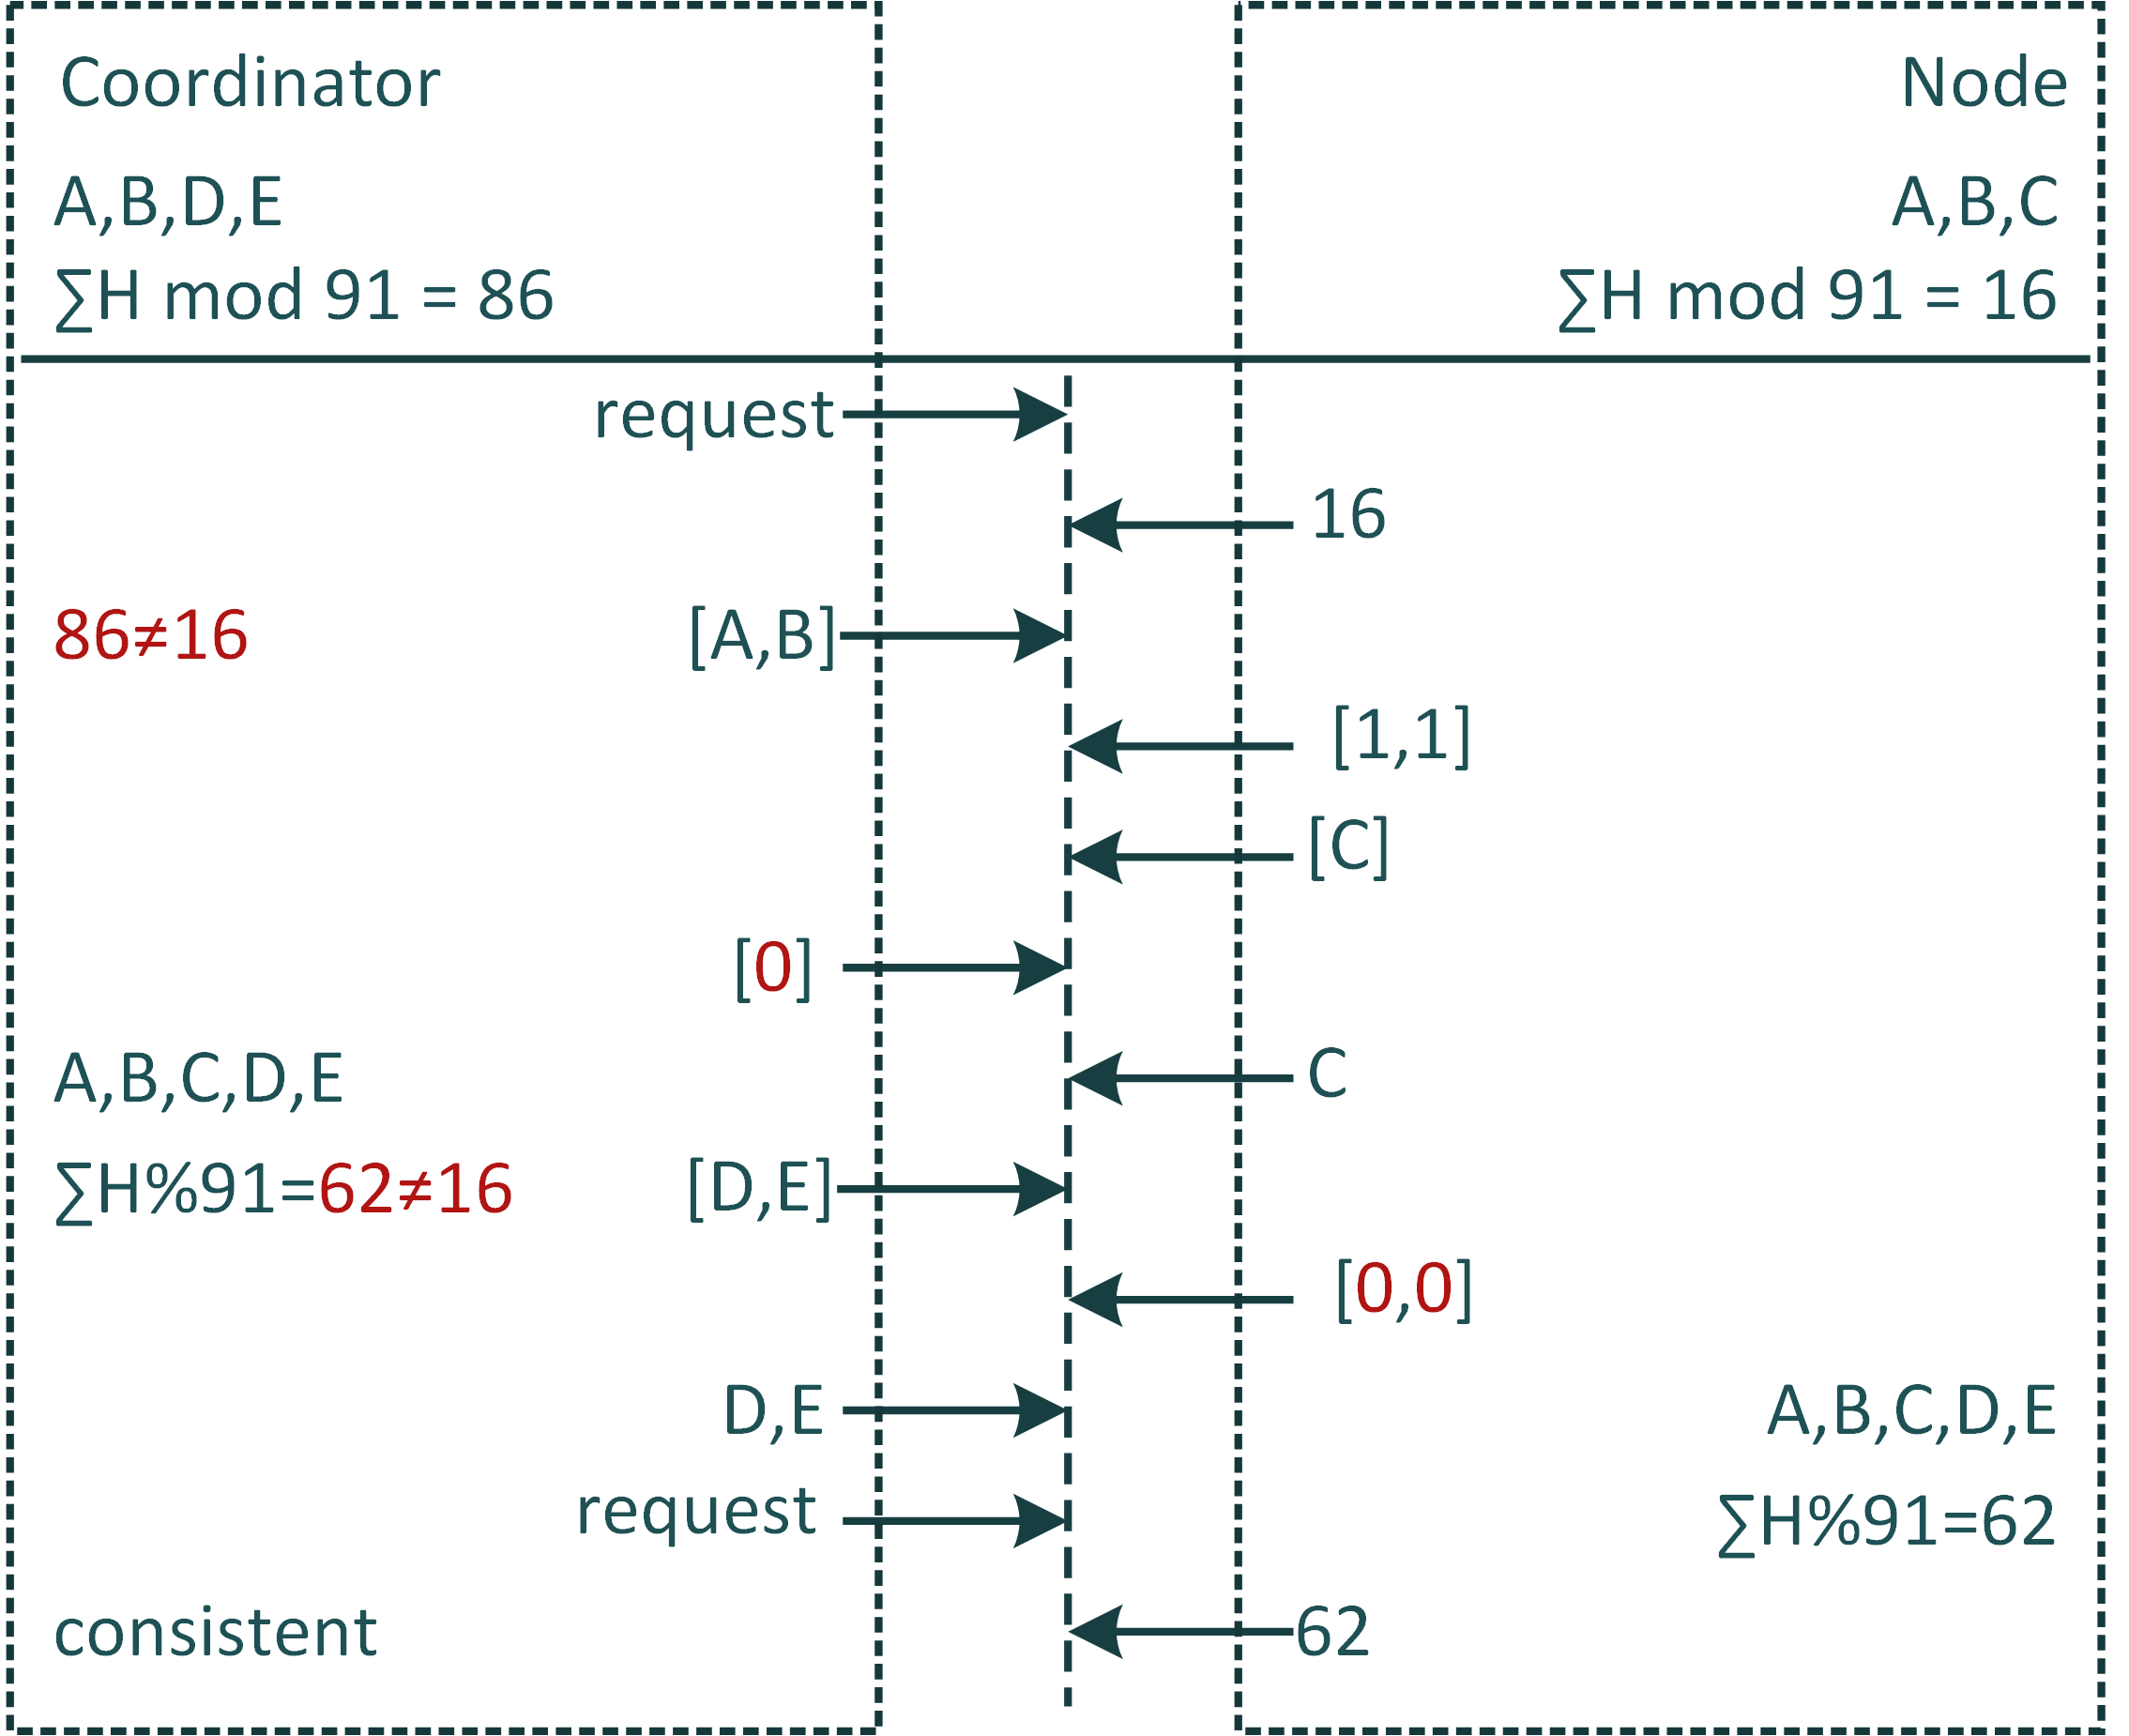
\includegraphics[scale=1.0]{figures/db-synchronization-ion.png}
\end{figure}

\subsection{Securing the Communication Channel} \label{Securing the Communication Channel}

As requested in requirement \ref{req:SMPC Module} and noted in \ref{Secure Addition Protocol} the \gls{SMPC} protocols need secure communication channels. Listen in on wireless communication means receiving the radio signals, so for common wireless technologies this is easily accomplished. Since the physical layer is more or less public, the communication needs encryption. 
For this framework two kinds of encryption are used: first asymmetric cryptography is used to exchange a session-key, which is then used to secure messages with symmetric encryption, as displayed in figure \ref{figure:RSA/AES scheme}. This principle is well known from \gls{TLS} encryption used in \gls{HTTPS}. For the asymmetric encryption the public-key cryptosystem \acs{RSA} as described by \textcite[pp. 49-76]{Delfs2015} is used. For the symmetric encryption the \gls{AES} as described by \textcite[pp. 19-25]{Delfs2015} is used.
\gls{AES} encrypts and decrypts faster than \gls{RSA}, because \gls{RSA} requires long keys (2048 bit and longer recommended) for proper security. But \gls{AES} needs sender and receiver to know the shared/symmetric key, and the exchange of this key over an insecure channel only with \gls{AES} is not possible.

\begin{figure}[!htbp] % h for placement here
	\caption{Securing communication with \gls{RSA} and \gls{AES}} \label{figure:RSA/AES scheme}
	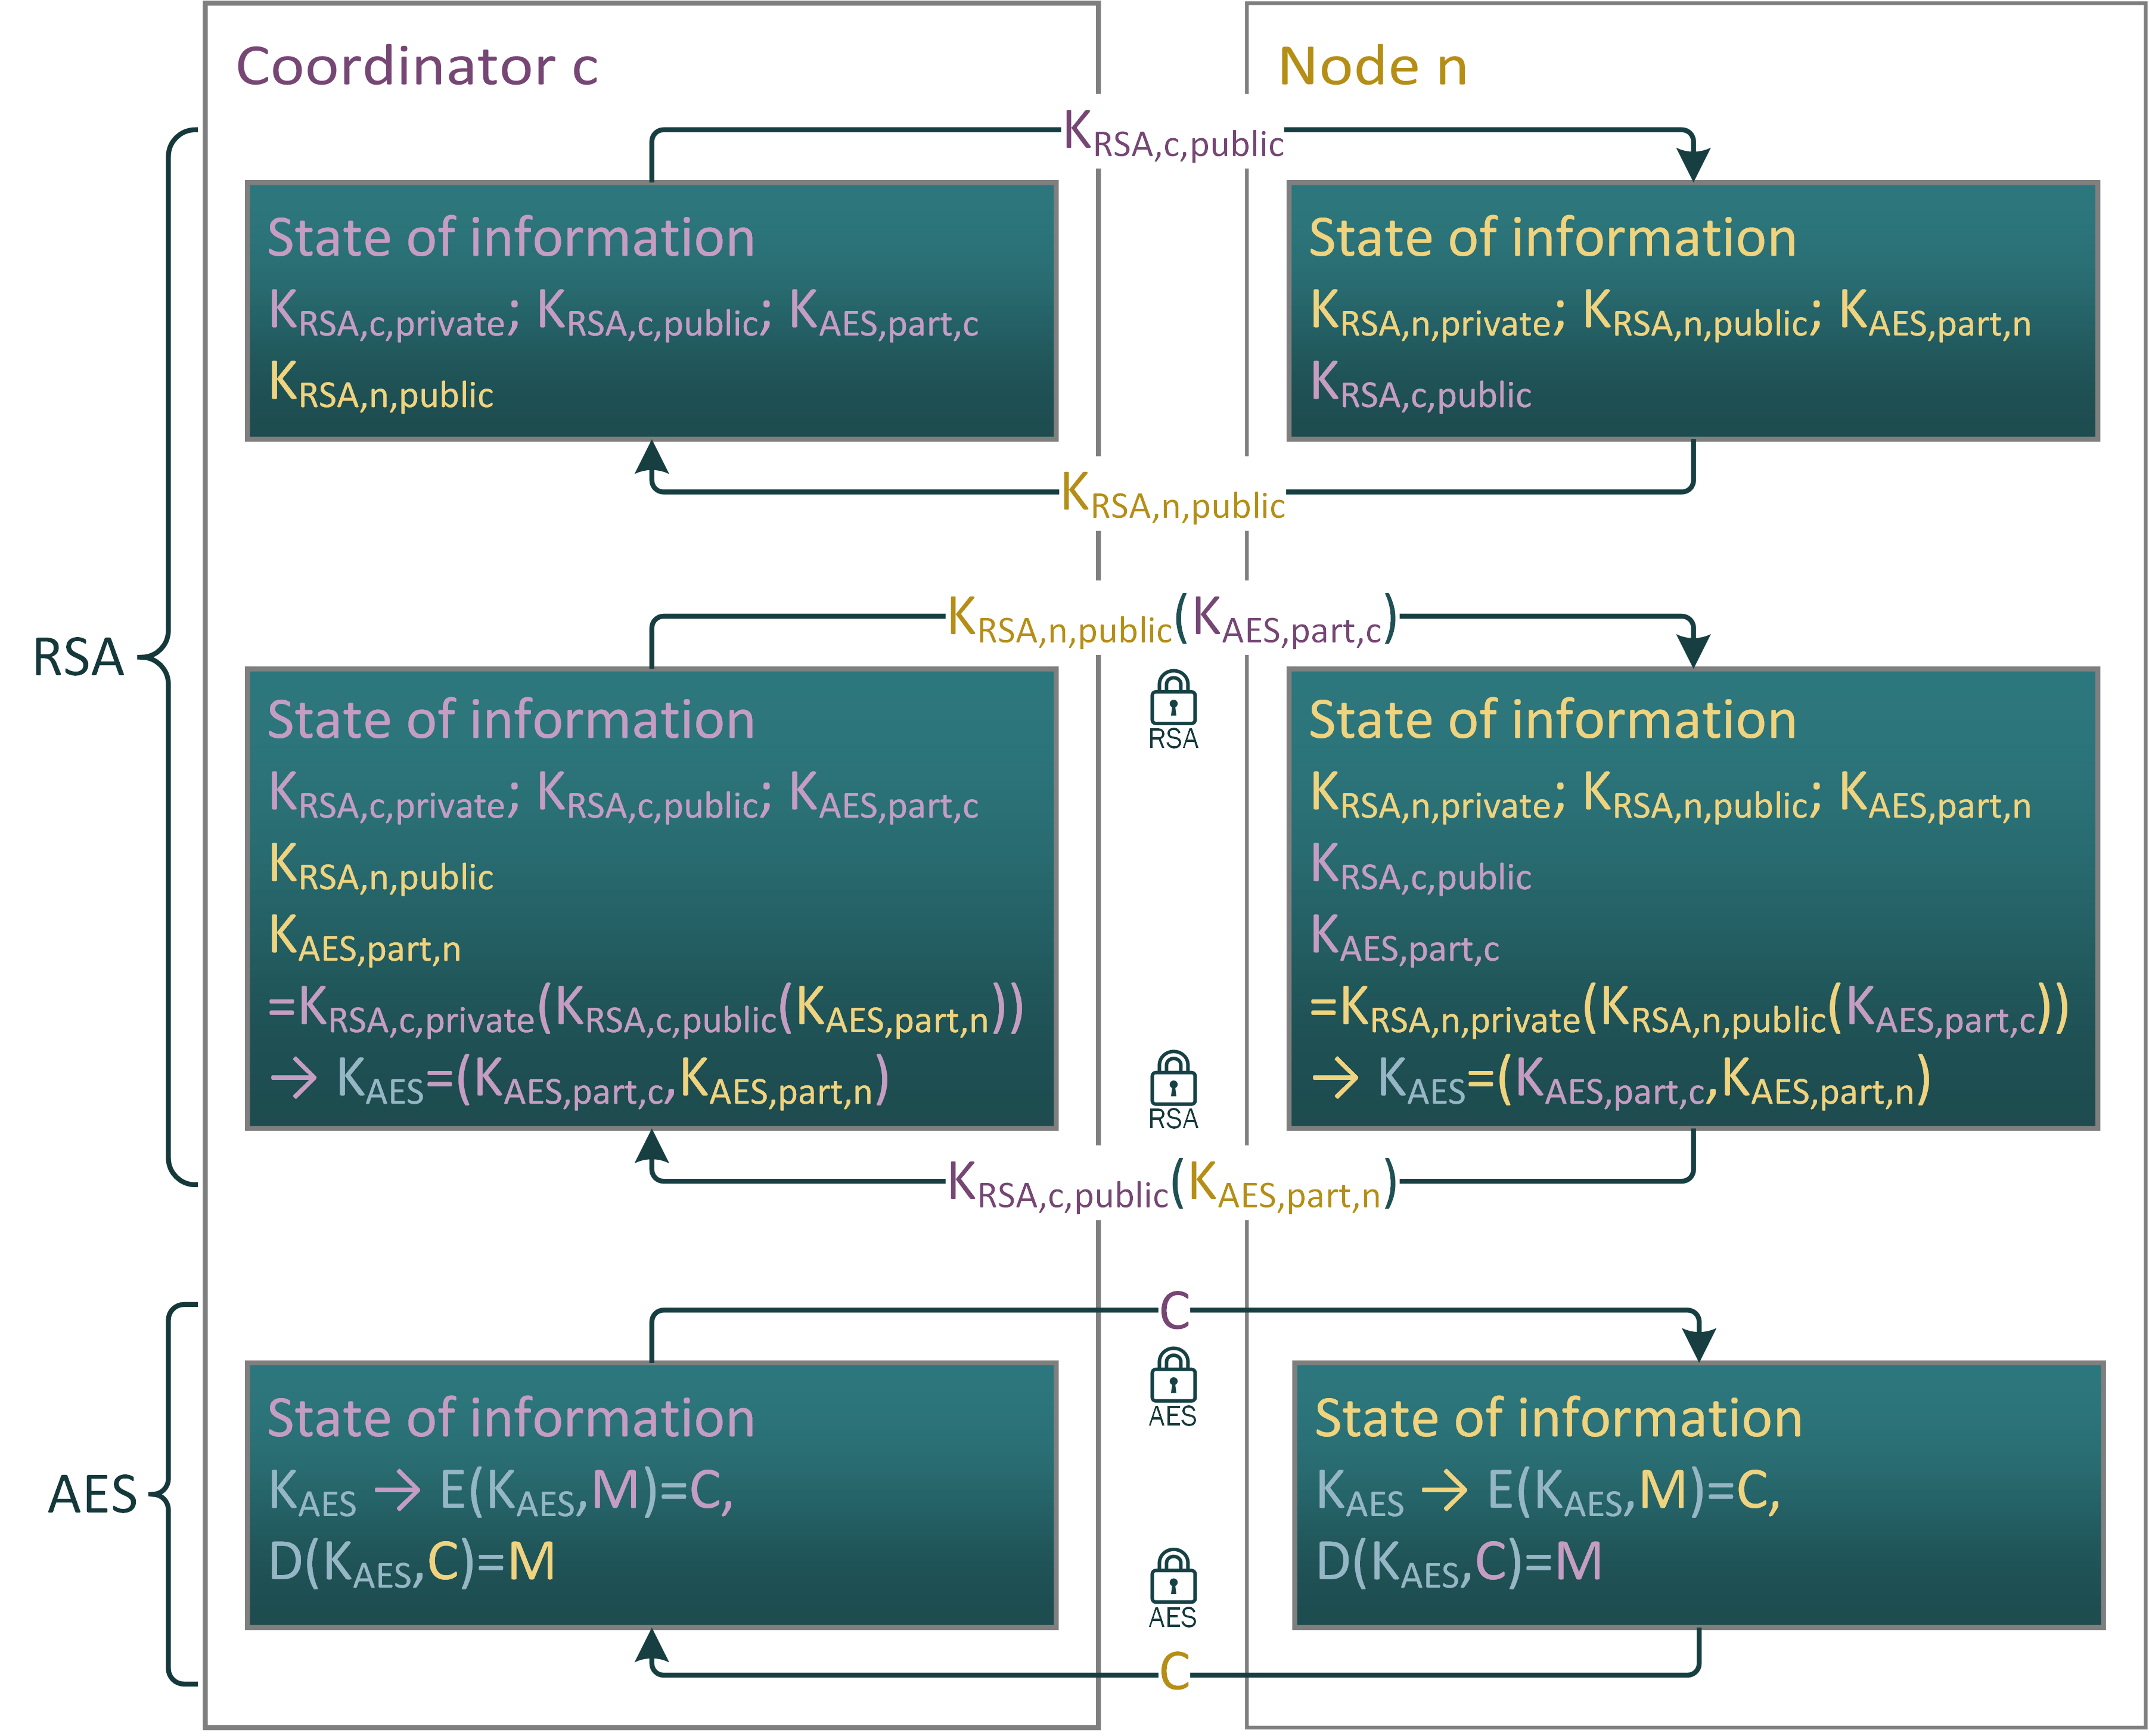
\includegraphics[scale=1.0]{figures/encryption-ion.png}
\end{figure}

The basis for the cryptosystem by \gls{RSA} is the prime-factorization, which requires super-polynomial time. \gls{RSA} is asymmetric, since there is one key for encryption and one key for decryption. In this setting, the public key is used for encryption, so only the receiver with the private key can decrypt the secret.
For the key generation two large prime numbers are selected: $p,q \in \gls{doubleP} \ \text{with} \ p\neq q$. The product $n=p\cdot q$ is computed. Euler's Phi function $\phi (n)=(p-1)(q-1)$ is computed and a coprime integer $e$ is selected $1<e<\phi(n)$. A common value for $e$ is $65537$. The public key is formed by $n$ and $e$.
The private key is formed from $n$ and $d$, where d meets $e\cdot d\equiv 1\mod \phi(n)$.

For the symmetric encryption, booth partners use the same key. \gls{AES} is an iterated block cipher with a block length of 128 bits and key length of 128, 192 or 256 bits. The iterations (called rounds) follow the Rijndael algorithm. A detailed description of the algorithm can be found in \textcite[pp. 20-25]{Delfs2015}.

\section{Architecture} \label{Architecture}

Based on \ref{Coordinator Election} it is sensible, that the central element in this framework is a node component. Figure \ref{figure:UML component diagram} displays the \gls{UML} component diagram for the framework design and illustrates the basic conjunctions between the components, as well as key-functionalities. The node component can also act as the coordinator and in either state communications and computations let it pass through different states of activity. This framework therefore uses the state pattern: the current state determines the behavior and abilities of the node.
In regard to the hosting system the node component utilizes an \gls{API} component, which uses callbacks to bind the communication layer and the system clock to the framework in accordance with \ref{req:Supportability}. To handle the message encryption a cryptography module is needed, providing the functionality described in \ref{Securing the Communication Channel}. As described in \ref{Non-termination Detection} a handler for timeout detection and heartbeat message triggering is provided. Parameters for communication, cryptography and \gls{SMPC} need to be accessible in a central component to meet \ref{req:Usability}.

\begin{figure}[!htbp] % h for placement here
	\caption{\gls{UML} component diagram} \label{figure:UML component diagram}
	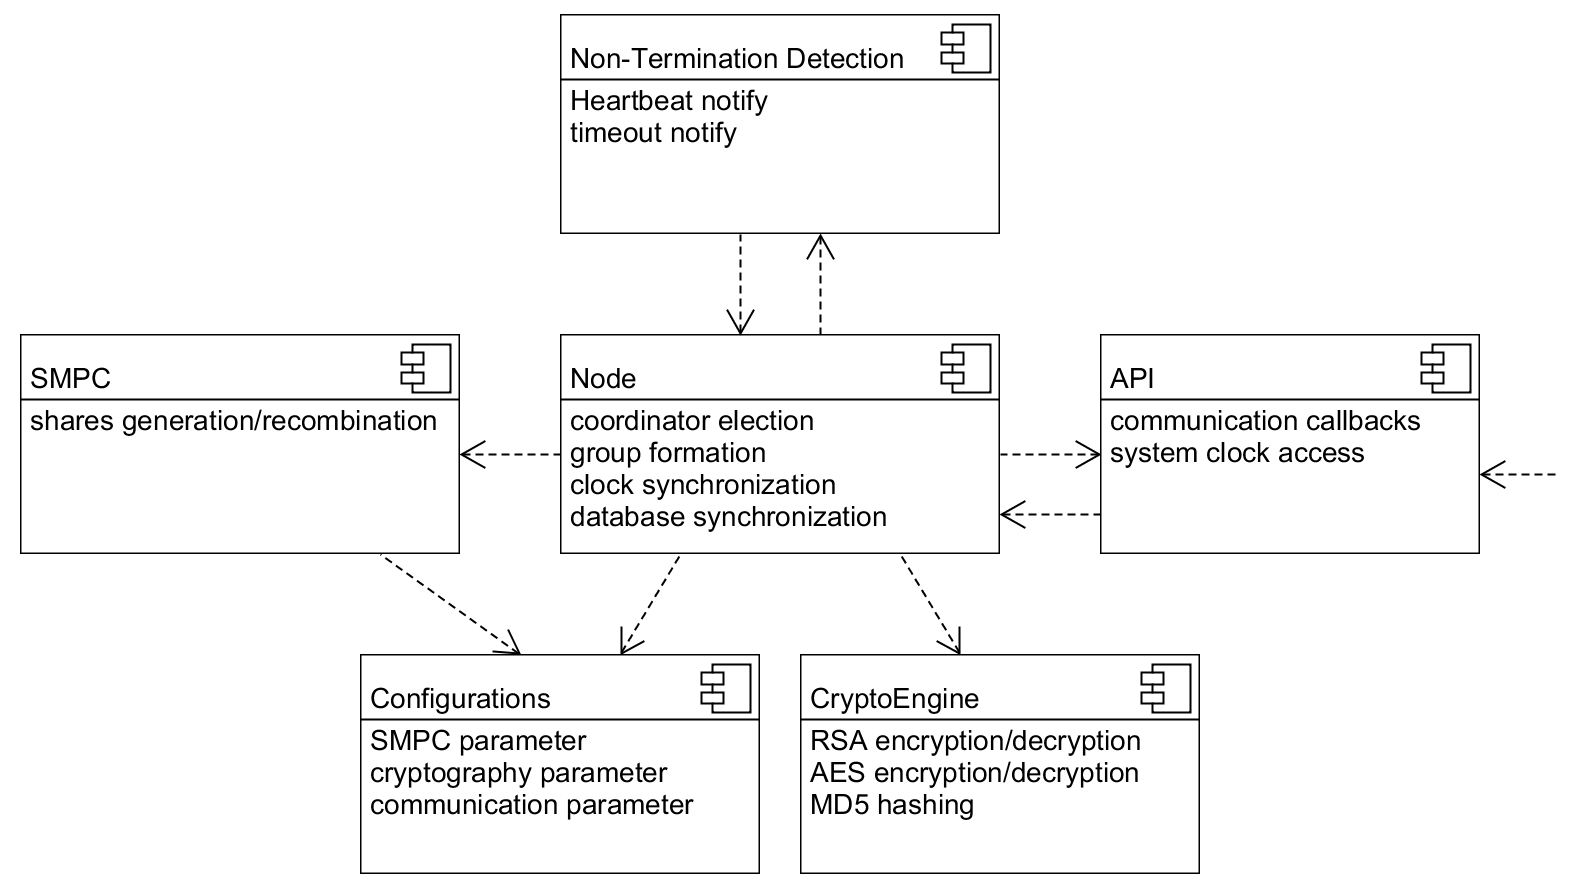
\includegraphics[scale=1.0]{figures/uml-component.png}
\end{figure}

Since it is likely, that the technical limitations described in \autoref{practicability of an implementation} will be overcome in future releases, the framework's core functionality is independent from the efforts to provide the self-forming network abilities (avoidance of code smell known as change preventer or shotgun surgery). So in case of availability of full \gls{MANET} capabilities (secure multi-hop routing and parallel communications) only the node component has to be adopted.

%\todo*{state machine; state pattern; client server architecture; \gls{UML} state diagrams for 1. joining network (get time; set clock delta), 2. finding computation partners, 3. running computation, 4. compare database}


\chapter{Implementation} \label{Implementation}

\todo*{15-20\%; details on the implementation; for someone who wants to continue the work}

While the algorithms and protocols described in \autoref{Background} and \autoref{Design} are language-independent, it is sensible to use the programming language C for the development, since it is widely supported on most \glspl{OS} including embedded \glspl{OS}. 
To evaluate the practicability of the proposed framework design for real-life usage, the core system is implemented.
To simplify the utilization and further development of the framework, first the development environments and tools used for the implementation of the core system are described.

Since the project will be hosted as an open-source project alongside a generated \gls{API}, important features of the modules are introduced along with notes regarding experienced problems.

\section{Development Tools}	\label{Development Tools}

The core implementation was developed on Arch Linux using the \gls{GCC} version 6.2.1. JetBrains CLion 2016.3.1 was selected as \gls{IDE}, because it is cross-platform, offers code completion and analysis and supports Doxygen.

Doxygen is a tool for generating documentation based on annotated sources (\autoref{Doxygen function annotation}), similar to Javadoc. Maintaining the documentation in the source files simplifies the process of keeping the documentation up to date after code changes and the documentation generation can be included in the build pipeline. This helps to avoid version conflicts between \gls{API} and source code, since developers can generate the \gls{API} on their local system from the sources, guaranteeing that the documentation at hand is the correct one for the used release of the source code. Doxygen offers the documentation as \gls{HTML} (\autoref{Doxygen function documentation}) and LaTeX, making it easy to provide platform independent documentation.

\begin{lstlisting}[language=C, caption={Doxygen function annotation}, label={Doxygen function annotation}]
/*!
Computes the modulo x mod p based on the cryptographic modulo definition.
\param x is an integer and the dividend.
\param p is an integer and the divisor.
\return The remainder of x mod p as an unsigned integer.
*/
unsigned int mod (long long x, int p);
\end{lstlisting}

\begin{figure}[!htbp] % h for placement here
	\caption{Doxygen function documentation} \label{Doxygen function documentation}
	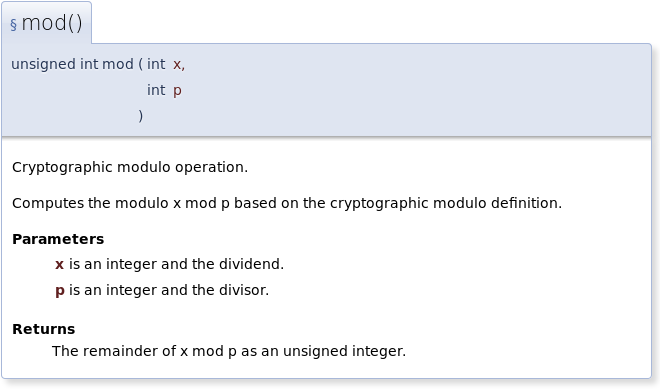
\includegraphics[scale=1.4]{figures/doxygen.png}
\end{figure}

For managing changes to documents, the distributed version control git is used and the project is hosted on GitHub. Besides providing access to the project and easy maintainability the intention is to let other developers suggest improvements using pull requests.

To validate the correctness of implemented functions, the unit test library Unity\footnote{\url{https://github.com/ThrowTheSwitch/Unity}} is used as a submodule. Using the parameter \lstinline|--recursive| the GitHub repository for Unity is embedded in the Security Games repository. 

For unit tests with Unity, test files are added to the project including validations of predefined test cases with known output (\autoref{Unity test file}). When build for testing (\lstinline|make test|), the defined tests are executed and the results are displayed (\autoref{Unity test result}).

\begin{lstlisting}[language=C, caption=Unity test file, label={Unity test file}, float,floatplacement=H]
#include "../src/SMPC_math.h"
#include "../lib/Unity/src/unity.h"

void test_mod(void)
{
	/* All of these should pass */
	TEST_ASSERT_EQUAL(1779, mod(-2255,2017));
	TEST_ASSERT_EQUAL(238, mod(2255,2017));
}

int main(void)
{
	UNITY_BEGIN();
	RUN_TEST(test_mod);
	return UNITY_END();
}
\end{lstlisting}

\begin{lstlisting}[language=C, caption={Unity test result}, label={Unity test result}, float, floatplacement=H]
test/SMPC_math_test.c:30:test_mod:PASS
-----------------------
1 Tests 0 Failures 0 Ignored 
OK
\end{lstlisting}


\section{Module Structure} \label{Module Structure}

As described in \autoref{Architecture} the central module for the framework is the Node module. The header file \lstinline|node.h| provides the interface to the host system. Settings and parameters for communication and computation are defined in \lstinline|configurations.h|. For the usage of the framework only those two header files are relevant: the settings in \lstinline|configurations.h| need to be adjusted to the use-case and  \lstinline|node.h| needs to be included in the own source file, to access functions and register function pointers for needed callbacks.
The core implementation contains the following files:

\begin{itemize}
	\item \lstinline|node.h|: provides function prototypes for setting function pointers for callbacks from the framework to host functions as well as function prototypes for passing massages to the framework.
	\item \lstinline|node.c| contains the implementation for the functions defined in \lstinline|node.h| and is the central managing unit. The processed messages define states for the node and it acts accordingly (state machine).
	\item \lstinline|configurations.h| is the central place for settings regarding network and computation parameters. Booth \lstinline|node.c| and \lstinline|smpc.c| access the definitions in \lstinline|configurations.h| and no other files need adjustment for the usage of the system.
	\item \lstinline|smpc.h| provides function prototypes to \lstinline|node.c| for the generation of the share matrix, the computation of the shares for the different \gls{SMPC} types and the Lagrange interpolation for recombination of shares.
	\item \lstinline|smpc.c| provides the implementation of the functions defined in \lstinline|smpc.h| as well as needed helper functions like the cryptographic modulo operation for negative values and fractions.
	\item wolfCrypt\footnote{\url{https://www.wolfssl.com/wolfSSL/Products-wolfcrypt.html}} cryptography engine provides asymmetric \gls{RSA} as well as symmetric \gls{AES} encryption (\lstinline|rsa.h, aes.h, random.h|) for securing the communication.
\end{itemize}

\subsection{Node Module} \label{Node Module}

The node module is the core of the framework and the only module interacting with the host system (see \autoref{Interfacing the Library}). Since nodes handle the formation of the computation group, they need to be aware of the host's identity, namely the \gls{MAC}, therefore the host passes the \gls{MAC} to the node when initializing it.

For the computation group a share matrix is required, that describes which nodes share secrets when the threshold for needed shares ($k$) is lower than the computation group size. The share matrix is a symmetric matrix with same row-sum and column-sum for all rows and columns. For example \autoref{Share matrix for secret sharing} displays the share matrix for $n=5$ and $k=3$ (so at least three shares are required for the Lagrange interpolation and two adversaries can be tolerated), where node $n_3$ will send his shares $s_{3,1}$ to $n_1$, $s_{3,3}$ to itself and $s_{3,5}$ to $s_5$ while receiving $s_{1,3}$ $s_{3,3}$ and $s_{5,3}$.
\begin{table}[]
	\centering
	\caption[Share matrix for secret sharing]{Share matrix for secret sharing with threshold}
	\label{Share matrix for secret sharing}
	\begin{tabular}{l|lllll}
		& 1 & 2 & 3 & 4 & 5 \\ \hline
		1 & 0 & 0 & 1 & 1 & 1 \\
		2 & 0 & 1 & 0 & 1 & 1 \\
		3 & 1 & 0 & 1 & 0 & 1 \\
		4 & 1 & 1 & 0 & 1 & 0 \\
		5 & 1 & 1 & 1 & 0 & 0
	\end{tabular}
\end{table}

To compute the share matrix, the number of nodes in the computation group needs to be known. The framework offers the setting for varying values for the minimum and the maximum computation group size. Small group sizes make it more likely that a computation is completed, in contrast larger group sizes improve the security. In general it is advised to settle for a value and define minimum and maximum group size with it. This enables the node to compute also all shares needed for the \gls{SMPC} computations without the interaction with other nodes and the online phase can be minimized (see \autoref{Off-line preparation for online computation}).

Once the host system passes a score to the node, the behavior of the node is controlled by different states. \autoref{Node module state machine} displays a simplified state diagram for coordinators and regular nodes once a score is passed.

\begin{figure}[!htbp] % h for placement here
	\caption{Off-line preparation for online computation} \label{figure:Off-line preparation for online computation}
	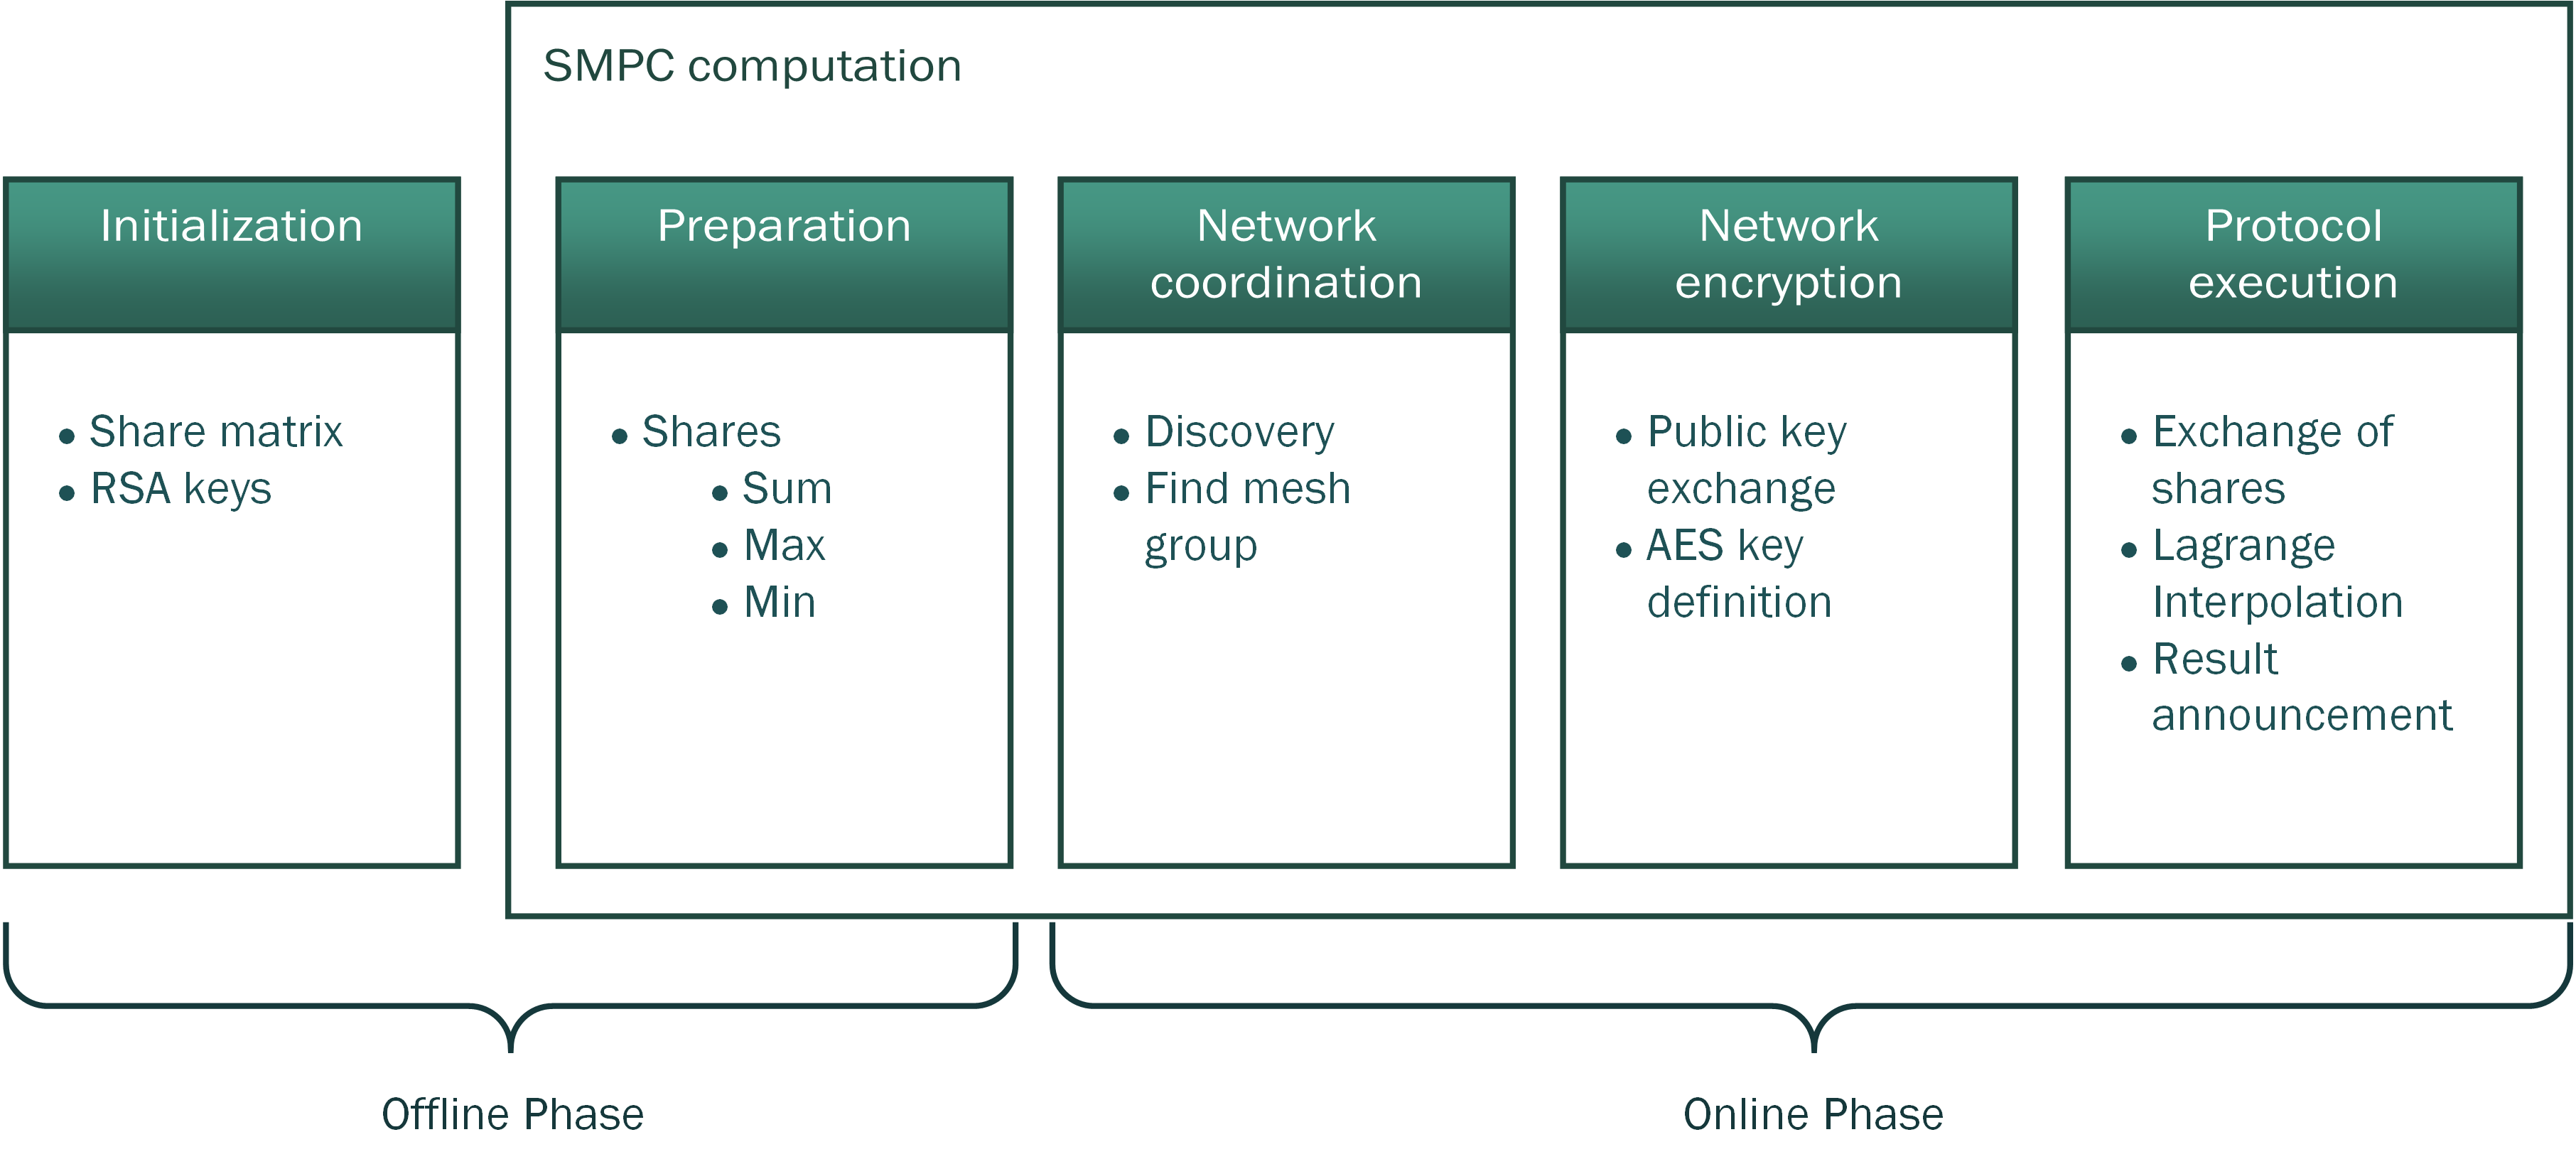
\includegraphics[scale=1.0]{figures/node_phases.png}
\end{figure}

\begin{figure}[!htbp] % h for placement here
	\caption{Node module state machine} \label{Node module state machine}
	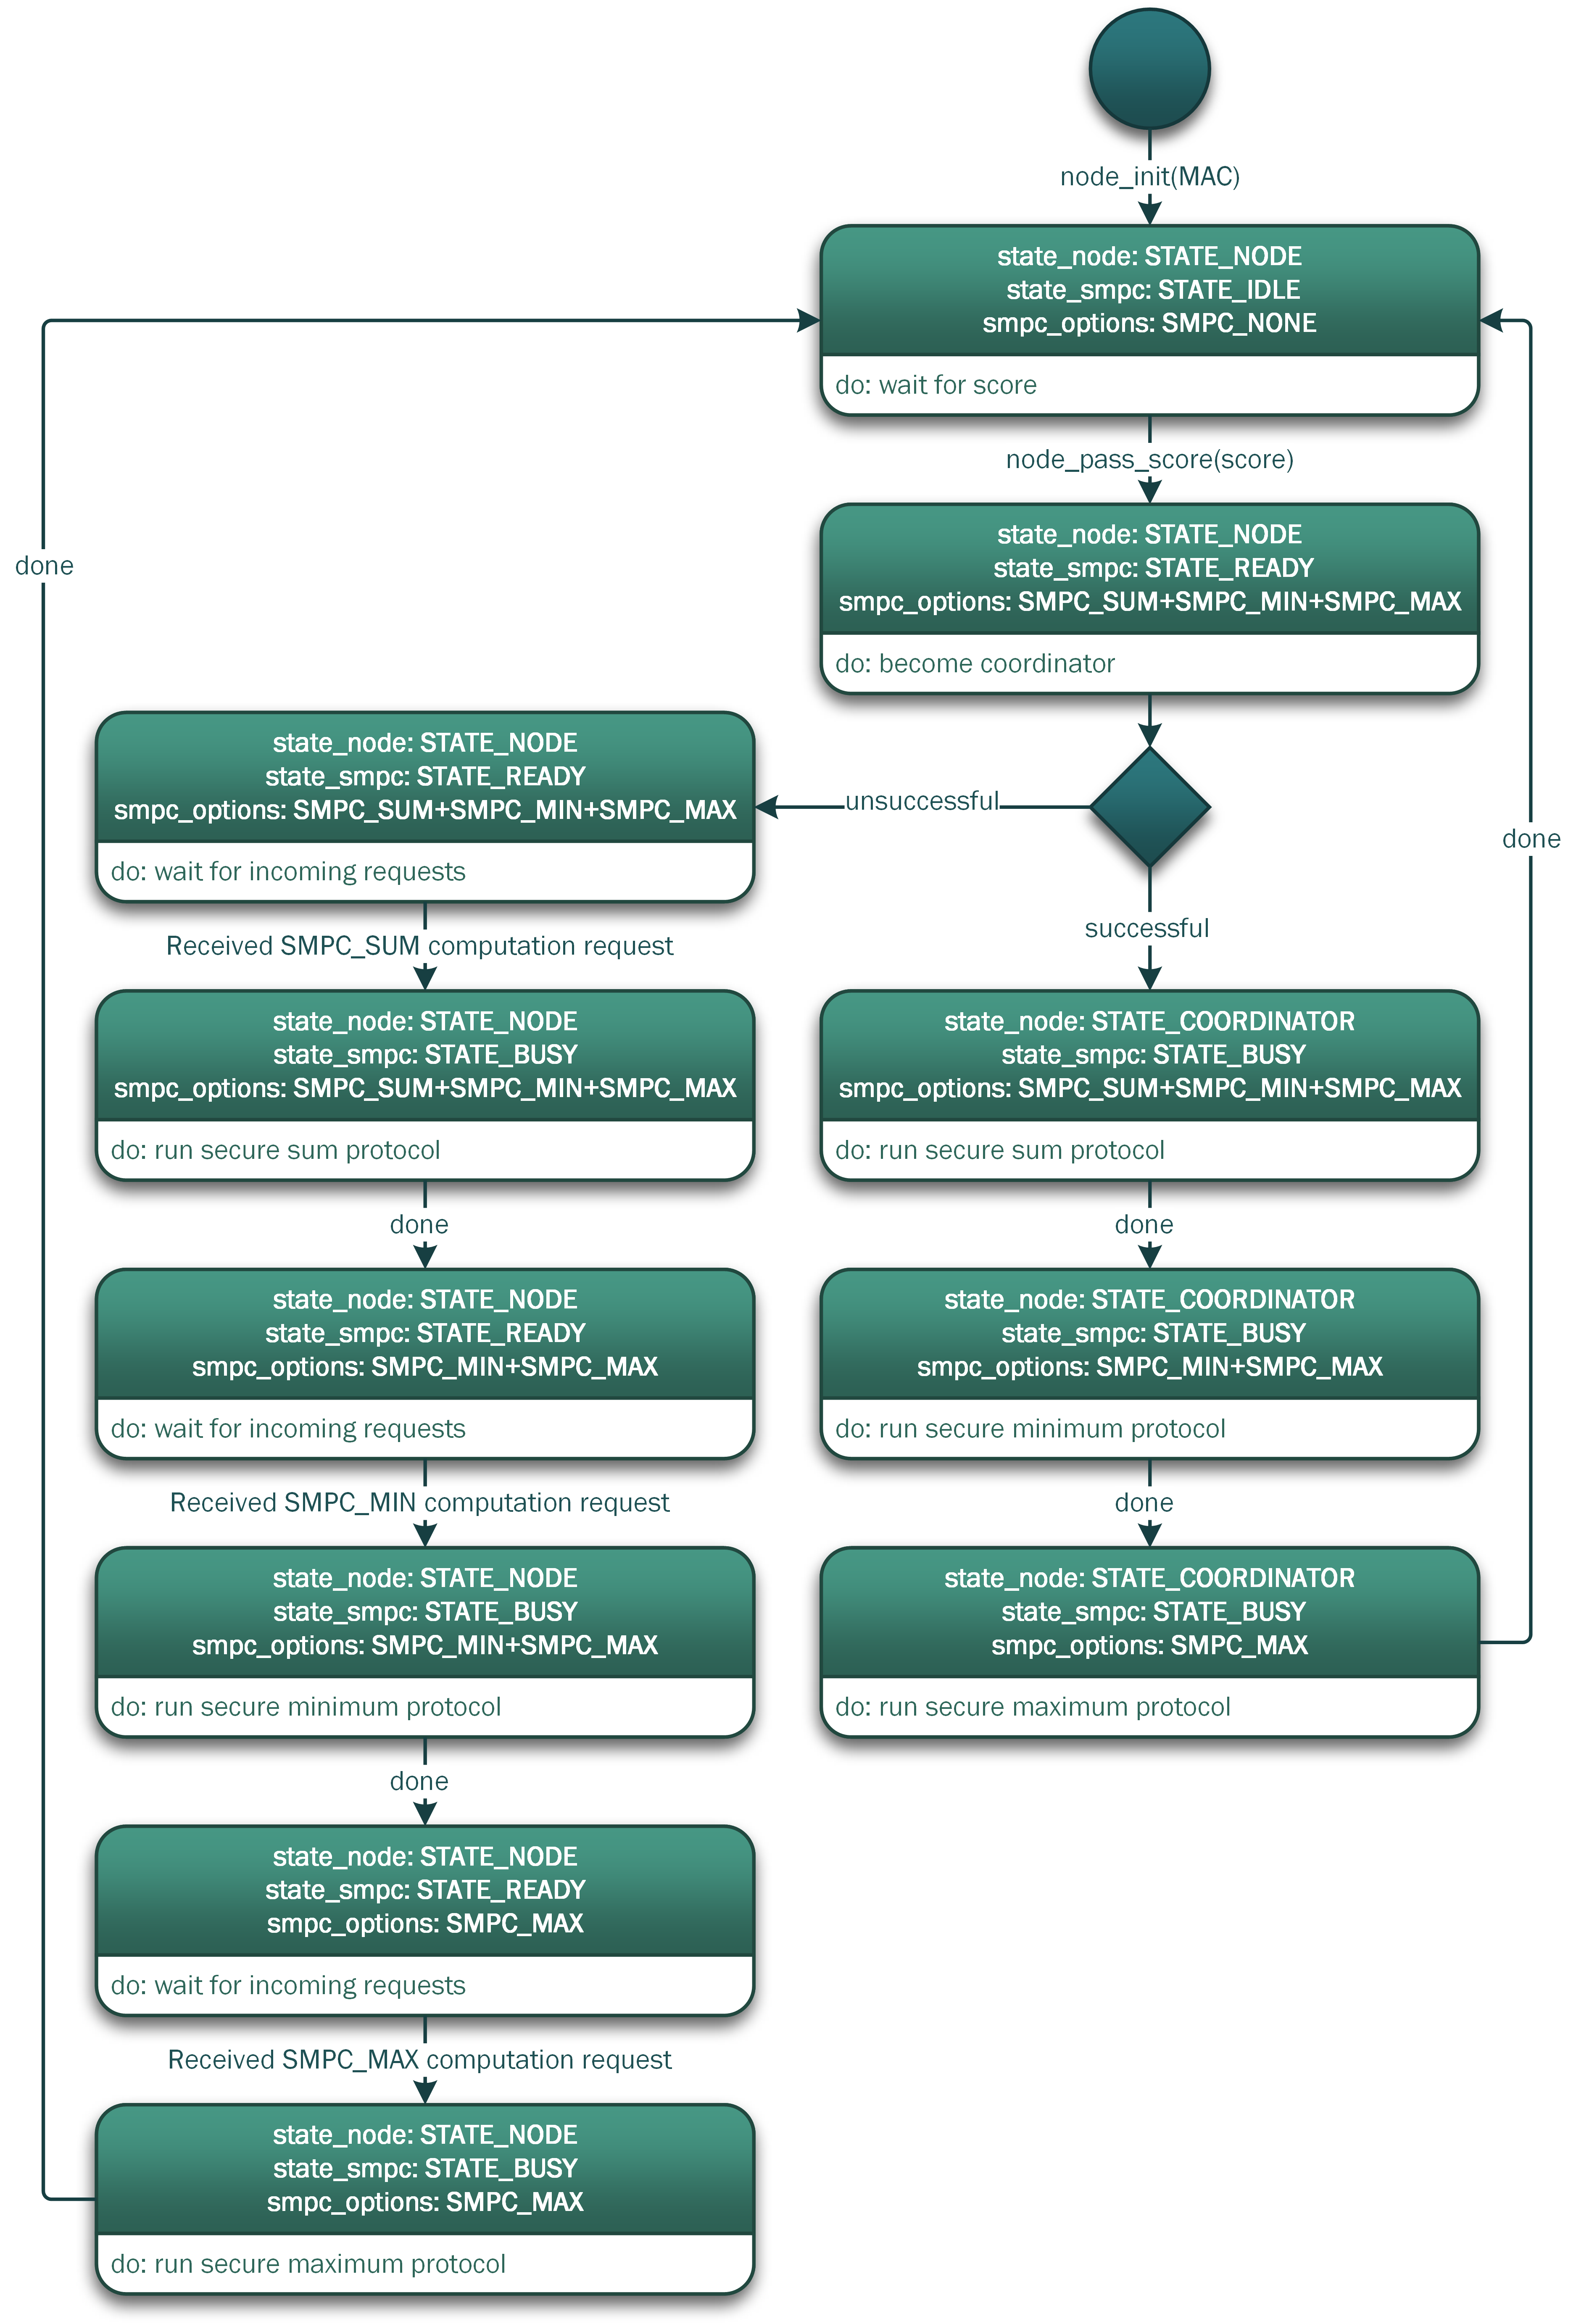
\includegraphics[scale=1.0]{figures/node_states.png}
\end{figure}

\subsubsection{Message Protocol} \label{Message Protocol}

Initialized by the coordinator, nodes pass messages between each other.
The normal communication flow is:
\begin{enumerate}
	\item send request
	\item await response
	\item handle response
\end{enumerate}

To identify the purpose of a received message, an enumeration for message types is implemented, avoiding magic numbers and providing readable condition checks.

\begin{lstlisting}[language=C, caption={Message type enumeration}, label={Message type enumeration}, float, floatplacement=H]
typedef enum { BROADCAST, ACK, STATE_REQUEST, STATE_RESPONSE, DISCOVERY_START_REQUEST, ... COMPUTATION_RESULT_RESPONSE } type_message;
\end{lstlisting}

Even though a regular broadcasting is not provided by the network (compare \autoref{practicability of an implementation}), the node module provides a pseudo-broadcast: a broadcast request requires a direct acknowledgment as a response. This was implemented to trigger longer processes, like discovery in all nodes in a more parallel way, instead of waiting for each node. 
For a broadcast the communication flow is:

\begin{enumerate}
	\item For each node in a passed list
	\begin{enumerate}
		\item send broadcast request: start long action
		\item await \lstinline|ACK|
	\end{enumerate}
	\item For each node in a passed list
		\begin{enumerate}
		\item send request: get result of long action
		\item await response
	\end{enumerate}
\end{enumerate}

The receiving node checks for each incoming message if the message begins with the broadcast enumerator, and responds with the \lstinline|ACK|, before reading and handling the additionally contained enumerator for the task request.

All messages are byte arrays (respectively char arrays), with varying length, depending on the payload (see \autoref{Message body}).

\begin{table}[]
	\centering
	\caption{Message body}
	\label{Message body}
	\begin{tabular}{|l|l|l|}
		\hline
		\lstinline|BROADCAST| (optional) & \lstinline|_REQUEST| or \lstinline|_RESPONSE| & Payload (optional) \\ \hline
	\end{tabular}
\end{table}

The transmitted \gls{SMPC} shares are encrypted using \gls{AES} encryption provided by the cryptography module.

\subsection{Cryptography Module: wolfCrypt} \label{Cryptography Module}

The cryptography engine wolfCrypt is open-source (GPLv2) and was selected because of the following reasons:

\begin{itemize}
	\item Provides asymmetric encryption with \gls{RSA} (for exchanging the symmetric key)
	\item Provides symmetric encryption with \gls{AES} (for exchanging encrypted messages)
	\item Provides hash algorithms, which will be utilized for the database features
	\item Lightweight library, usable on embedded systems (e.g. \gls{TI-RTOS})
\end{itemize}

Like the Unity framework, wolfCrypt is referenced int the repository as a submodule. Using the parameter \lstinline|--recursive| the GitHub repository for Unity is embedded in the Security Games repository, ensuring relative paths in header includes and in the makefile are preserved. Submodules also reference a specific commit, so build errors through different source code versions can be reduced.

To meet up-to-date security demands (see \autoref{Securing the Communication Channel}), \gls{RSA} keys of length 3072 bits are generated and \gls{AES} keys with 192 bit are used (see \autoref{Configuration}) as defaults, though changes can be made in \lstinline|configurations.h|.

For the generation of the \gls{RSA} private key \lstinline|WOLFSSL_API int wc_MakeRsaKey(RsaKey* key, int size, long e, WC_RNG* rng);| is used, which is only available when \lstinline|WOLFSSL_KEY_GEN| is defined, therefore \lstinline|rsa.o| is compiled with the \lstinline|-DWOLFSSL_KEY_GEN| option.

Specific required modules from the library are embedded in the framework but not altered or extended, hence for further information the extensive wolfCrypt documentation\footnote{\url{https://www.wolfssl.com/wolfSSL/Docs-wolfssl-manual-18-wolfcrypt-api-reference.html}} can be consulted.

\subsection{Secure Multi-Party Computation Module} \label{SMPC Module}

The \gls{SMPC} module provides functions to create shares for the secure sum, minimum and maximum computation. As described in \autoref{Secure Comparison Protocol} the shares for following rounds change, when a node disqualifies itself as the maximum. For the off-line preparation the \gls{SMPC} module therefore generates for each computation round additional shares for the disqualification case.
For large computation groups and large upper limits for the maximum score storage has to be considered, especially when running the framework on embedded system. 
\begin{alignat}{3}
\intertext{For example, the upper bound for the maximum score is 10000 and the computation group has a size of 20 and scores are 4 byte integers:}
&n=20, \  b_{10}=10000 && \Rightarrow && b_2=10 \ 0111 \ 0001 \ 0000 \nonumber \\
&\text{Secure sum:} \ && \text{1 round:} \quad && 20\cdot4\text{ byte}=80\text{ byte} \nonumber \\
&\text{Secure max:} \ && \text{14 rounds:} \quad && 14\cdot 20 \cdot 4\text{ byte}=1120\text{ byte} \nonumber \\
&\text{Secure max disqualified:} \ && \text{14 rounds:} \quad && 14\cdot 20 \cdot 4\text{ byte}=1120\text{ byte} \nonumber \\
&\text{Secure min:} \ && \text{14 rounds:} \quad && 14\cdot 20 \cdot 4\text{ byte}=1120\text{ byte} \nonumber \\
&\text{Secure min disqualified:} \ && \text{14 rounds:} \quad && 14\cdot 20 \cdot 4\text{ byte}=1120\text{ byte} \nonumber
\intertext{In total: $4560$ byte need to be stored for the given example values.} \nonumber
\end{alignat}
The \gls{SMPC} module also offers the restoration of the secret using Lagrange interpolation (see \autoref{Public function prototypes in smpc.h}). The interpretation of the result remains in the control of the node module. If the Lagrange interpolation for a round in the secure max protocol returns a value unequal to zero the node has to set the related bit for the maximum result and so on.

\begin{lstlisting}[language=C, caption={Public function prototypes in smpc.h}, label={Public function prototypes in smpc.h}, float, floatplacement=H]
void smpc_generate_shares(int shares[], int n, int k, int secret, smpc_share_type type);
int smpc_lagrange_interpolation(int involved_parties[], int shares[], int k);
\end{lstlisting}

All computations need to be in the finite ring defined by the upper bound prime. For lager computation groups the intermediate values in the Lagrange interpolation can leave the range, so potential risk operations have to be casted in a larger type and afterwards returned into the ring using modular operations. The \gls{SMPC} module therefore offers the cryptographic modulo for negative values and a modulo for fractions based on the Euclidean algorithm. Also for power operations with the risk of reaching undefined type ranges a power function with modulo application on intermediate values is provided (see \autoref{Modular operations in smpc.c})

\begin{lstlisting}[language=C, caption={Modular operations in smpc.c}, label={Modular operations in smpc.c}, float, floatplacement=H]
int mod_power(int base, int power, int mod);
unsigned int mod (long long , int );
int mod_fraction(long long x, int p);
\end{lstlisting}

\section{Interfacing the Library} \label{Interfacing the Library}

As mentioned in \autoref{Node Module} for the usage of the library \lstinline|node.h| provides the prototypes for function callbacks, that need to be provided from the host system, to give the library access to the communication layer. In the current implementation the system is intended for the usage with Bluetooth and devices are identified by \gls{MAC}, but with moderate effort the system is portable to an IP address based system: only the arrays containing the discovery results and related messages in the node module need adjustments, otherwise the computations are independent from the communication layer.
Based on tests on various Android device with different \gls{API} levels only the \gls{RFCOMM}Bluetooth protocol offers the ability to connect devices without (with minimum) user-interaction.

\subsection{Configuration} \label{Configuration}

Before the system is used, the settings in \lstinline|configuration.h| should be adjusted to the demands of the own system. The default values are displayed in \autoref{Definitions in configurations.h}.

\begin{lstlisting}[language=C, caption={Definitions in configurations.h}, label={Definitions in configurations.h}, float, floatplacement=H]
#define CONFIGURATIONS_MINIMUM_COMPUTATION_GROUP 20
#define CONFIGURATIONS_MAXIMUM_COMPUTATION_GROUP 20
#define CONFIGURATIONS_MAX_SCORE 10000
// wolfCrypt settings
#define CONFIGURATIONS_AES_KEY_SIZE 192
#define CONFIGURATIONS_RSA_KEY_SIZE 3072
#define CONFIGURATIONS_BOUNDING_PRIME 2147483647
\end{lstlisting}

As previously described the value for minimum and maximum computation group size are set to the same value, making the group size static and enabling the computation of the shares in the off-line phase (see \autoref{figure:Off-line preparation for online computation}). 

Smaller computation groups offer better performance and reduce the risk of network separation, but for security reasons no adversaries should be tolerated. Providing a narrow estimation for the possible scores thorough the maximum score value is important for the secure maximum and minimum protocols, because it determines the number of needed rounds.

The selected key sizes for \gls{RSA} and \gls{AES} meet currently considered secure settings.  

\subsection{Usage in C}	\label{Usage in C}

After including \lstinline|node.h| the host has access to the functions to initialize the node, pass a score or pass a message (see \autoref{Function prototypes int node.h}). 

\begin{lstlisting}[language=C, caption={Function prototypes int node.h}, label={Function prototypes int node.h}, float, floatplacement=H]
void node_init(char *mac);
void node_pass_score(int score);
void node_pass_message(char *source, char *message);
void node_set_discovery_function(void(*func)(char macs[][18], int* result_count));
void node_set_send_function(void(*func)(char *target, char *message));
void node_set_await_function(int (*func)(char * source, char[]));
\end{lstlisting}

Using the provided setters, the host system needs to provide the function pointers for the functions to send from the node, run discovery of Bluetooth devices and await the response from a specified node (see \autoref{Prototypes for host callbacks}). After setting the callbacks the node can be initialized before passing the first score (see \autoref{Node setup and system start}).

\begin{lstlisting}[language=C, caption={Prototypes for host callbacks}, label={Prototypes for host callbacks}, float, floatplacement=H]
void host_function_send_message(char *target, char *message);
void host_function_discovery(char macs[][18], int* result_count);
int host_function_await_response(char *source, char response[]);
\end{lstlisting}

\begin{lstlisting}[language=C, caption={Node setup and system start}, label={Node setup and system start}, float, floatplacement=H]
node_set_discovery_function(&host_function_discovery);
node_set_await_function(&host_function_await_response);
node_set_send_function(&host_function_send_message);
node_init(mac);
node_pass_score(score);
\end{lstlisting}


\subsection{Usage in Android} \label{Usage in Android}
Using the Android \gls{NDK} it is possible to utilize C and C++ libraries inside of activities, to reuse existing code base.

To develop native code for Android with Android Studio the following \gls{SDK} Tools are needed and are provided through the integrated \gls{SDK} Manager

\begin{itemize}
	\item LLDB: a debugger, providing debugging of native code to Android Studio
	\item CMake: an open-source, cross-platform build tool, working alongside the Gradle Build Tool embedded in Android Studio 
\end{itemize} 

To call functions from the library in Java code the function calls are wrapped in native methods implemented by the native-lib. The signature of the function is marked with the native keyword and the function name follows a strict naming convention.

\begin{lstlisting}[language=Java, caption={Method signature in MainActivity.java}, label={Method signature in MainActivity.java}, float, floatplacement=H]
public native void nodePassMessage(String source, String message);
\end{lstlisting}

\begin{lstlisting}[language=Java, caption={Function implementation in node\_wrapper.c}, label={Function implementation in node_wrapper.c}, float, floatplacement=H]
JNIEXPORT void JNICALL
Java_[package]_MainActivity_nodePassMessages(JNIEnv *env, jobject this, jstring source, jstring message) { ... }
\end{lstlisting}

\begin{figure}[!htbp] % h for placement here
	\caption{\gls{JNI} bridge between Java and C code} \label{JNI bridge between Java and C code}
	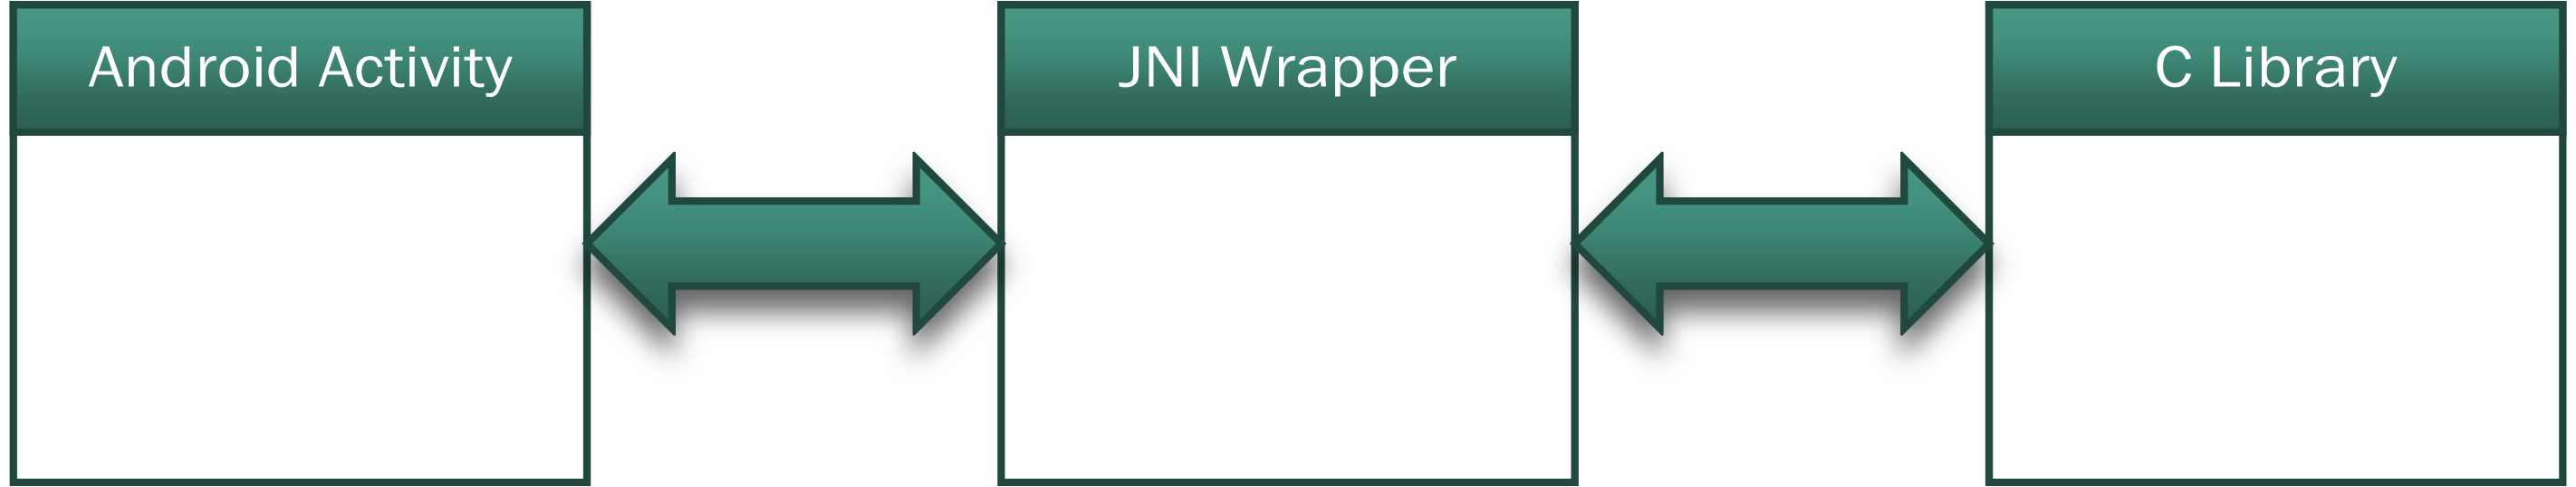
\includegraphics[scale=1.0]{figures/jni_wrapper.png}
\end{figure}

To provide a callback function, \gls{JNI} class lookup can be used. To call a Java method defined as \lstinline|public void sendMessage(String target, String message){ ... }| class and method references can be stored (see \autoref{Using a Java method as callback for native method}) and the reference to a wrapping function is passed to the C library.

\begin{lstlisting}[language=C, caption={Using a Java method as callback for native method}, label={Using a Java method as callback for native method}, float, floatplacement=H]
    jclass mainClass = (*env)->FindClass(env, "[package]/MainActivity");
jmethodID id = (*env)->GetMethodID(env, mainClass, "sendMessage", "(Ljava/lang/String;Ljava/lang/String;)V");
jobject javaObjectRef = (*env)->NewObject(env, mainClass, id);
(*env)->CallVoidMethod(javaObjectRef, id, "some mac", "some message");
\end{lstlisting}

\subsubsection{Android Bluetooth Observations} \label{Android Bluetooth Observations}

In regard to the implementation of the \gls{RFCOMM} communication, different versions of Android showed different behavior: when trying to set the visibility, older test devices running Android 4.0 up to Android 4.3 issued the initial user confirmation to become indefinitely discoverable (see \autoref{Android discoverable intent}), but stopped without notification after the duration set in the Bluetooth settings, deviation from the android documentation. In contrast Android 5 devices became discoverable indefinitely (until Bluetooth was disabled and re-enabled). 

\begin{lstlisting}[language=Java, caption={Android discoverable intent}, label={Android discoverable intent}, float, floatplacement=H]
Intent discoverableIntent = new Intent(BluetoothAdapter.ACTION_REQUEST_DISCOVERABLE);
discoverableIntent.putExtra(BluetoothAdapter.EXTRA_DISCOVERABLE_DURATION, 0);
context.startActivity(discoverableIntent);
\end{lstlisting}

Also one device (Kindle Fire HDX based on Android 4.2.2) showed unexpected behavior when establishing the insecure \gls{RFCOMM} connection, showing briefly the pairing request before hiding it, yet denying the connection. From these first tests - though not representative - the downward compatibility for devices running Android 4.3 and below might be problematic.

\FloatBarrier


\chapter{Evaluation} \label{Evaluation}
\todo*{5-15\%; outcome; how was it tested; for supervisor}

While the correctness of the implemented methods is verified using unit tests (see \autoref{Development Tools}), the influence of configurable options (see \fullref{Configuration}), like the group size has to be evaluated. Also the impact of devices with significant lower computation power is of interest when targeting wearables and \gls{IoT} grade devices.
For the usage of the framework embedded in an Android application running battery powered devices like the personal smartphone, the power consumption is also an important topic.

%\section{Testing Tools}	\label{Testing Tools}

%\todo*{centralized client-server test application for android: trigger test runs, report results (measured execution time, correctness)}

\section{Power Consumption for Bluetooth States} \label{Power Consumption for Bluetooth States}

To evaluate the power consumption of Android devices in different Bluetooth states an application was developed enabling Bluetooth states for a specific amount a time. Then a report can be imported from the devices which contains estimated power usage\footnote{\url{https://developer.android.com/studio/profile/battery-historian.html}}.

\begin{enumerate}
	\item Using \gls{ADB} with a connected device, the battery stats are reseted to reduce the produced analysis file to the duration of interest: \lstinline|adb shell dumpsys batterystats --reset|
	\item The device is disconnected from the development system, so battery stats are recorded
	\item The application is executed for a fixed time duration
	\item The device is reconnected to the development system and using \gls{ADB} the report is pulled from the device: \lstinline|adb bugreport > bugreport.txt|
	\item The report contains a section labeled estimated power use (see \autoref{Android battery stats report})
\end{enumerate}
  
\begin{lstlisting}[language=C, caption={Android battery stats report}, label={Android battery stats report}]
Estimated power use (mAh):
Capacity: 2300, Computed drain: 229, actual drain: 184-207
Screen: 146
Bluetooth: 12,0
\end{lstlisting}
  
All test were realized on a Sony Experia Z1 Compact:
\begin{itemize}
	\item Android 5.1.1
	\item Software Version 14.6.A.1.236
	\item disabled power saving modes
\end{itemize}   

Each test case has a runtime of one hour, to reduce the significance of measuring inaccuracy. At the beginning and after completion of the tests Bluetooth is disabled. Discoverable state is periodically verified during the test with another Android device in range. Tests:

\begin{enumerate}
	\item Bluetooth enabled, not discoverable, not discovering and not connected
	\item Bluetooth enabled, discoverable, not discovering and not connected
	\item Bluetooth enabled, discoverable, not discovering and connected over \gls{RFCOMM}
	\item Bluetooth enabled, discoverable, not discovering, connected over \gls{RFCOMM} and exchanging small messages
	\item Bluetooth enabled, discoverable, and discovering, not connected
	\item Wi-Fi enabled, connected and receiving video-stream
\end{enumerate}

The results of the power consumption tests are displayed in \autoref{figure:Batterystats}.

\begin{figure}[!htbp] % h for placement here
	\caption{Batterystats for different Bluetooth states (logarithmic scale) } \label{figure:Batterystats}
	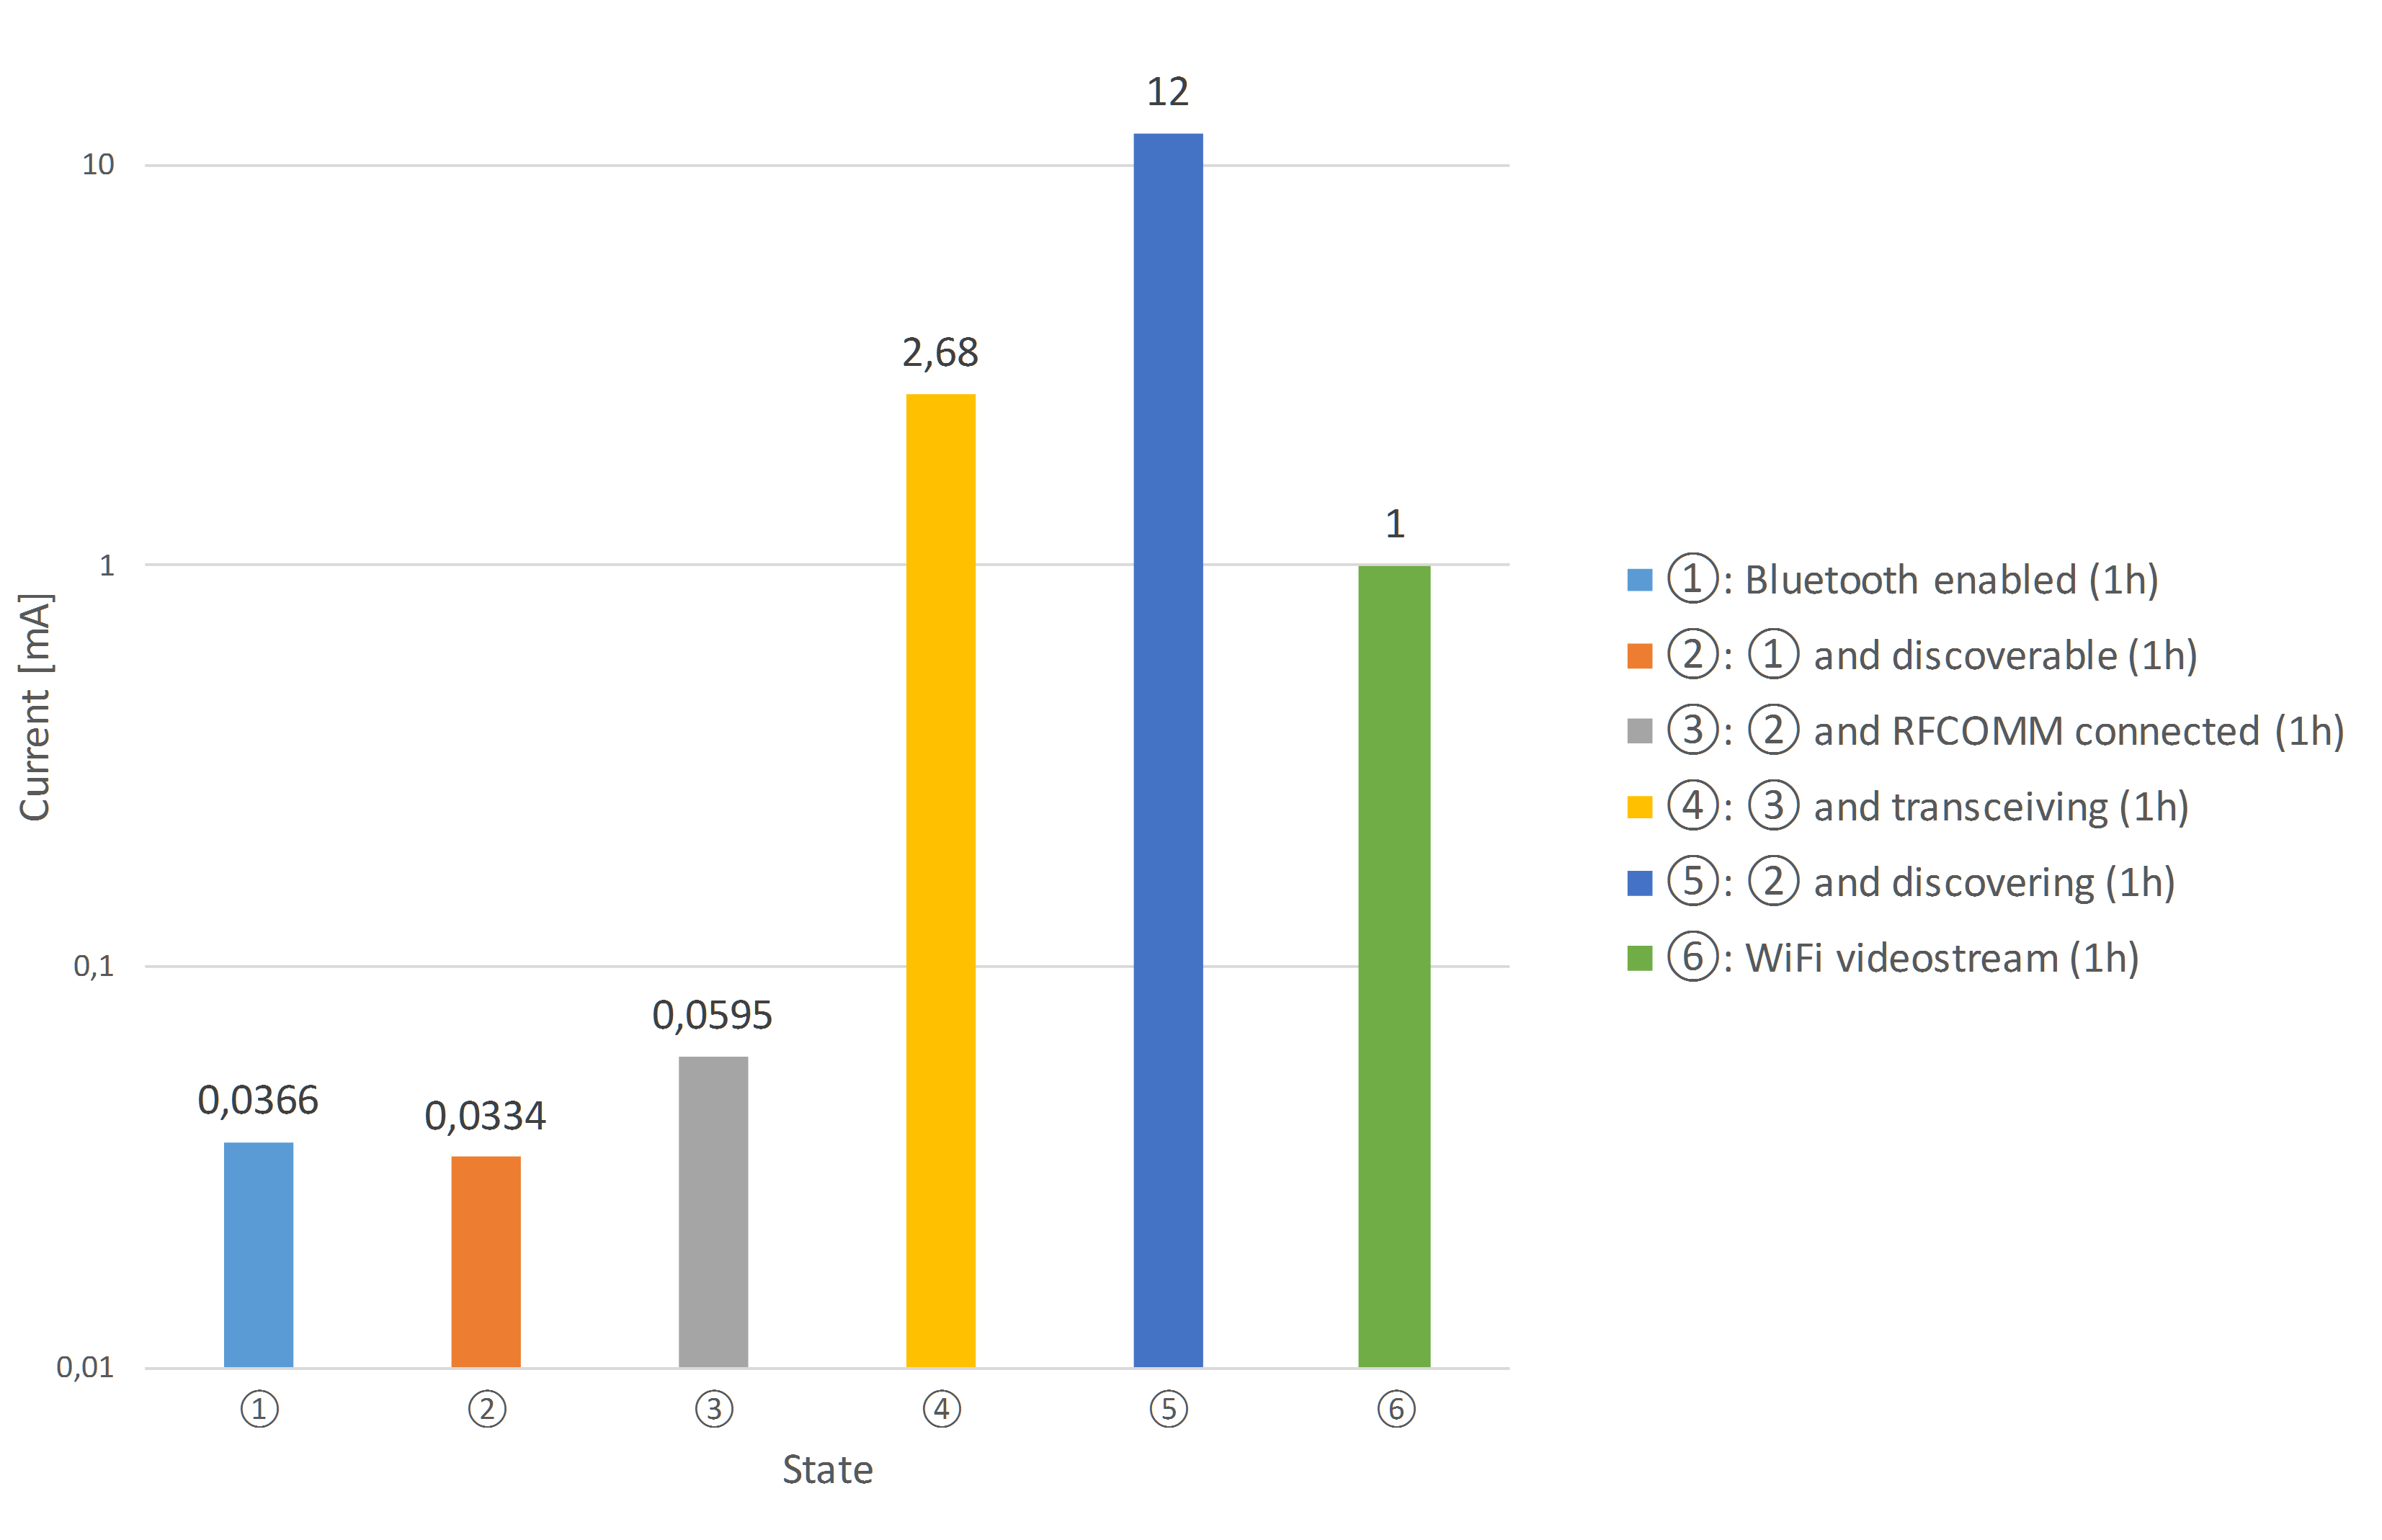
\includegraphics[scale=1.0]{figures/eval_current_measurements.png}
\end{figure}

\section{Examination of Computation Time Dependent on Number of Participants} \label{Examination of Computation Time Dependent on Number of Participants}

For the evaluation of the influence of computation power and computation group size a tester application was developed, that utilizes the framework by including node.h and providing the needed callbacks. Using a bash script, the group size $n$ can be passed as a parameter to the application and the script generates $n$ processes and assigns a \gls{MAC} to each process as well as a score value.

The processes communicate using named pipes, with the \gls{MAC} as name, so the communication flow is very similar to the communication over a \gls{RFCOMM} socket.

To take the discovery duration into account, the tester application forces a sleep for 3 seconds, when discovery is called by the node module. Also a sleep duration based on the lower end for Bluetooth transmission rates (732,2 kbit/s) is applied for outgoing messages depending on the message length.

The time critical part is the online phase of the computations (see \autoref{Off-line preparation for online computation}), therefore the coordinator measures the time (using the \lstinline|<time.h>| library) from sending the state request to all nodes nearby until the computation is concluded with the acknowledgment from all nodes in response to the computation result announcement.

Test settings for secure sum protocol:
\begin{enumerate}
	\item Secure sum with 5 nodes
	\item Secure sum with 10 nodes
	\item Secure sum with 20 nodes
	\item Secure sum with 40 nodes
	\item Secure sum with 80 nodes
	\item Secure sum with 100 nodes
\end{enumerate}

Test execution: each test was repeated three times and the displayed durations in \autoref{figure:Computation time over number of nodes for secure sum} and \autoref{figure:Computation time over number of nodes for secure maximum} are the arithmetic average to reduce the significance of disturbances through other processes.

\begin{figure}[!htbp] % h for placement here
	\caption{Computation time over number of nodes for secure sum} \label{figure:Computation time over number of nodes for secure sum}
	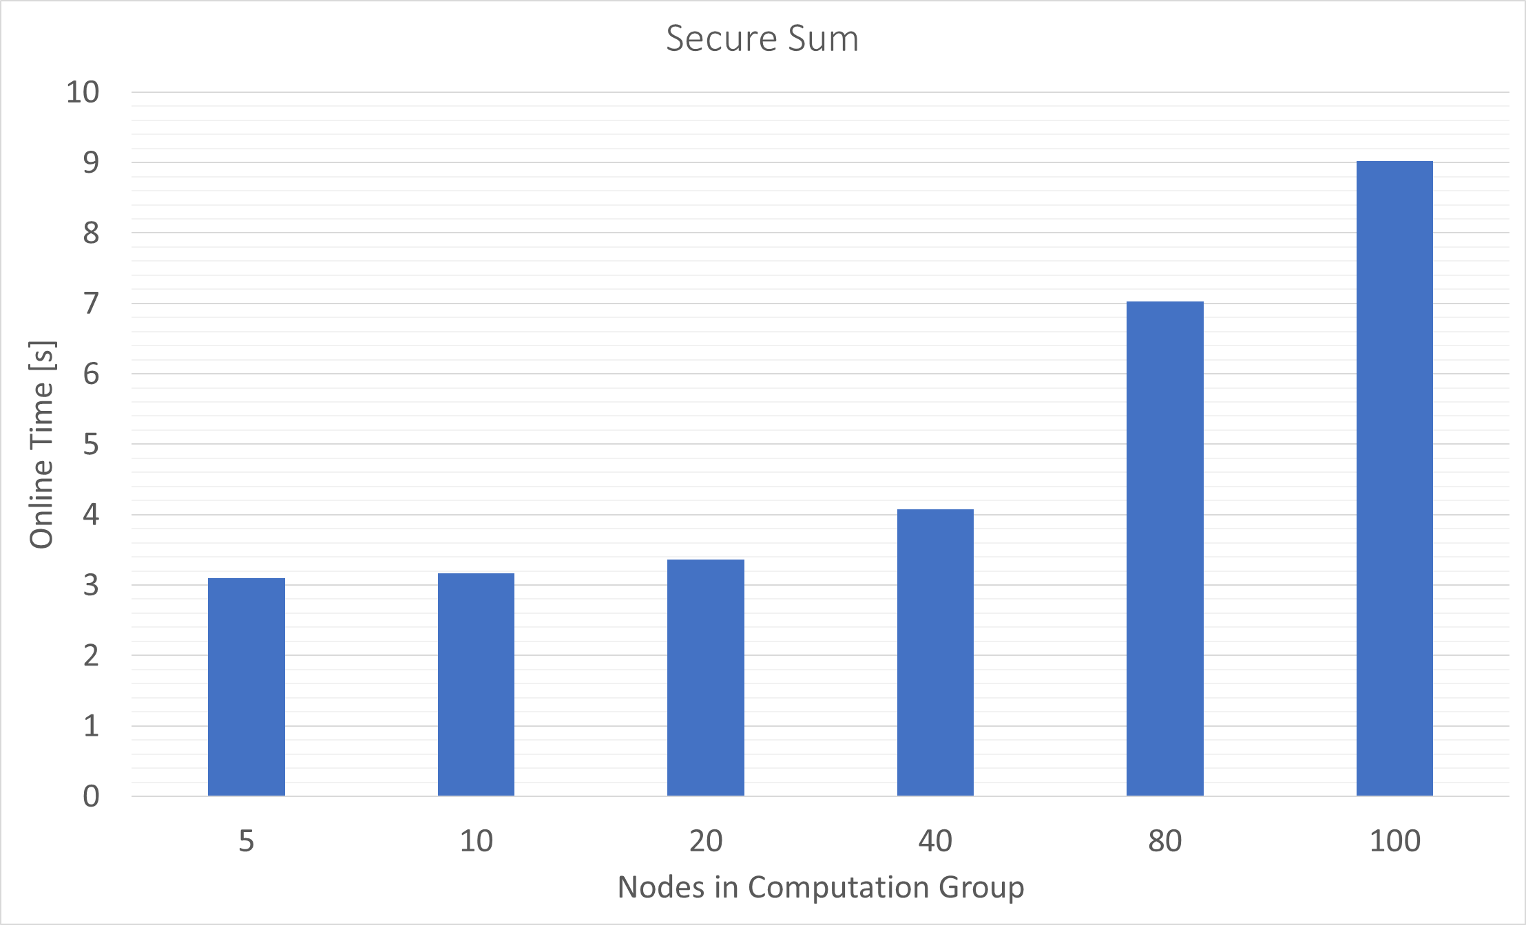
\includegraphics[scale=1.0]{figures/eval_sum.png}
\end{figure}

Test settings for secure maximum protocol:
\begin{enumerate}
	\item Secure minimum/maximum with 5 nodes
	\item Secure minimum/maximum with 10 nodes
	\item Secure minimum/maximum with 20 nodes
	\item Secure minimum/maximum with 40 nodes
	\item Secure minimum/maximum with 80 nodes
	\item Secure minimum/maximum with 100 nodes
\end{enumerate}


\begin{figure}[!htbp] % h for placement here
	\caption{Computation time over number of nodes for secure maximum} \label{figure:Computation time over number of nodes for secure maximum}
	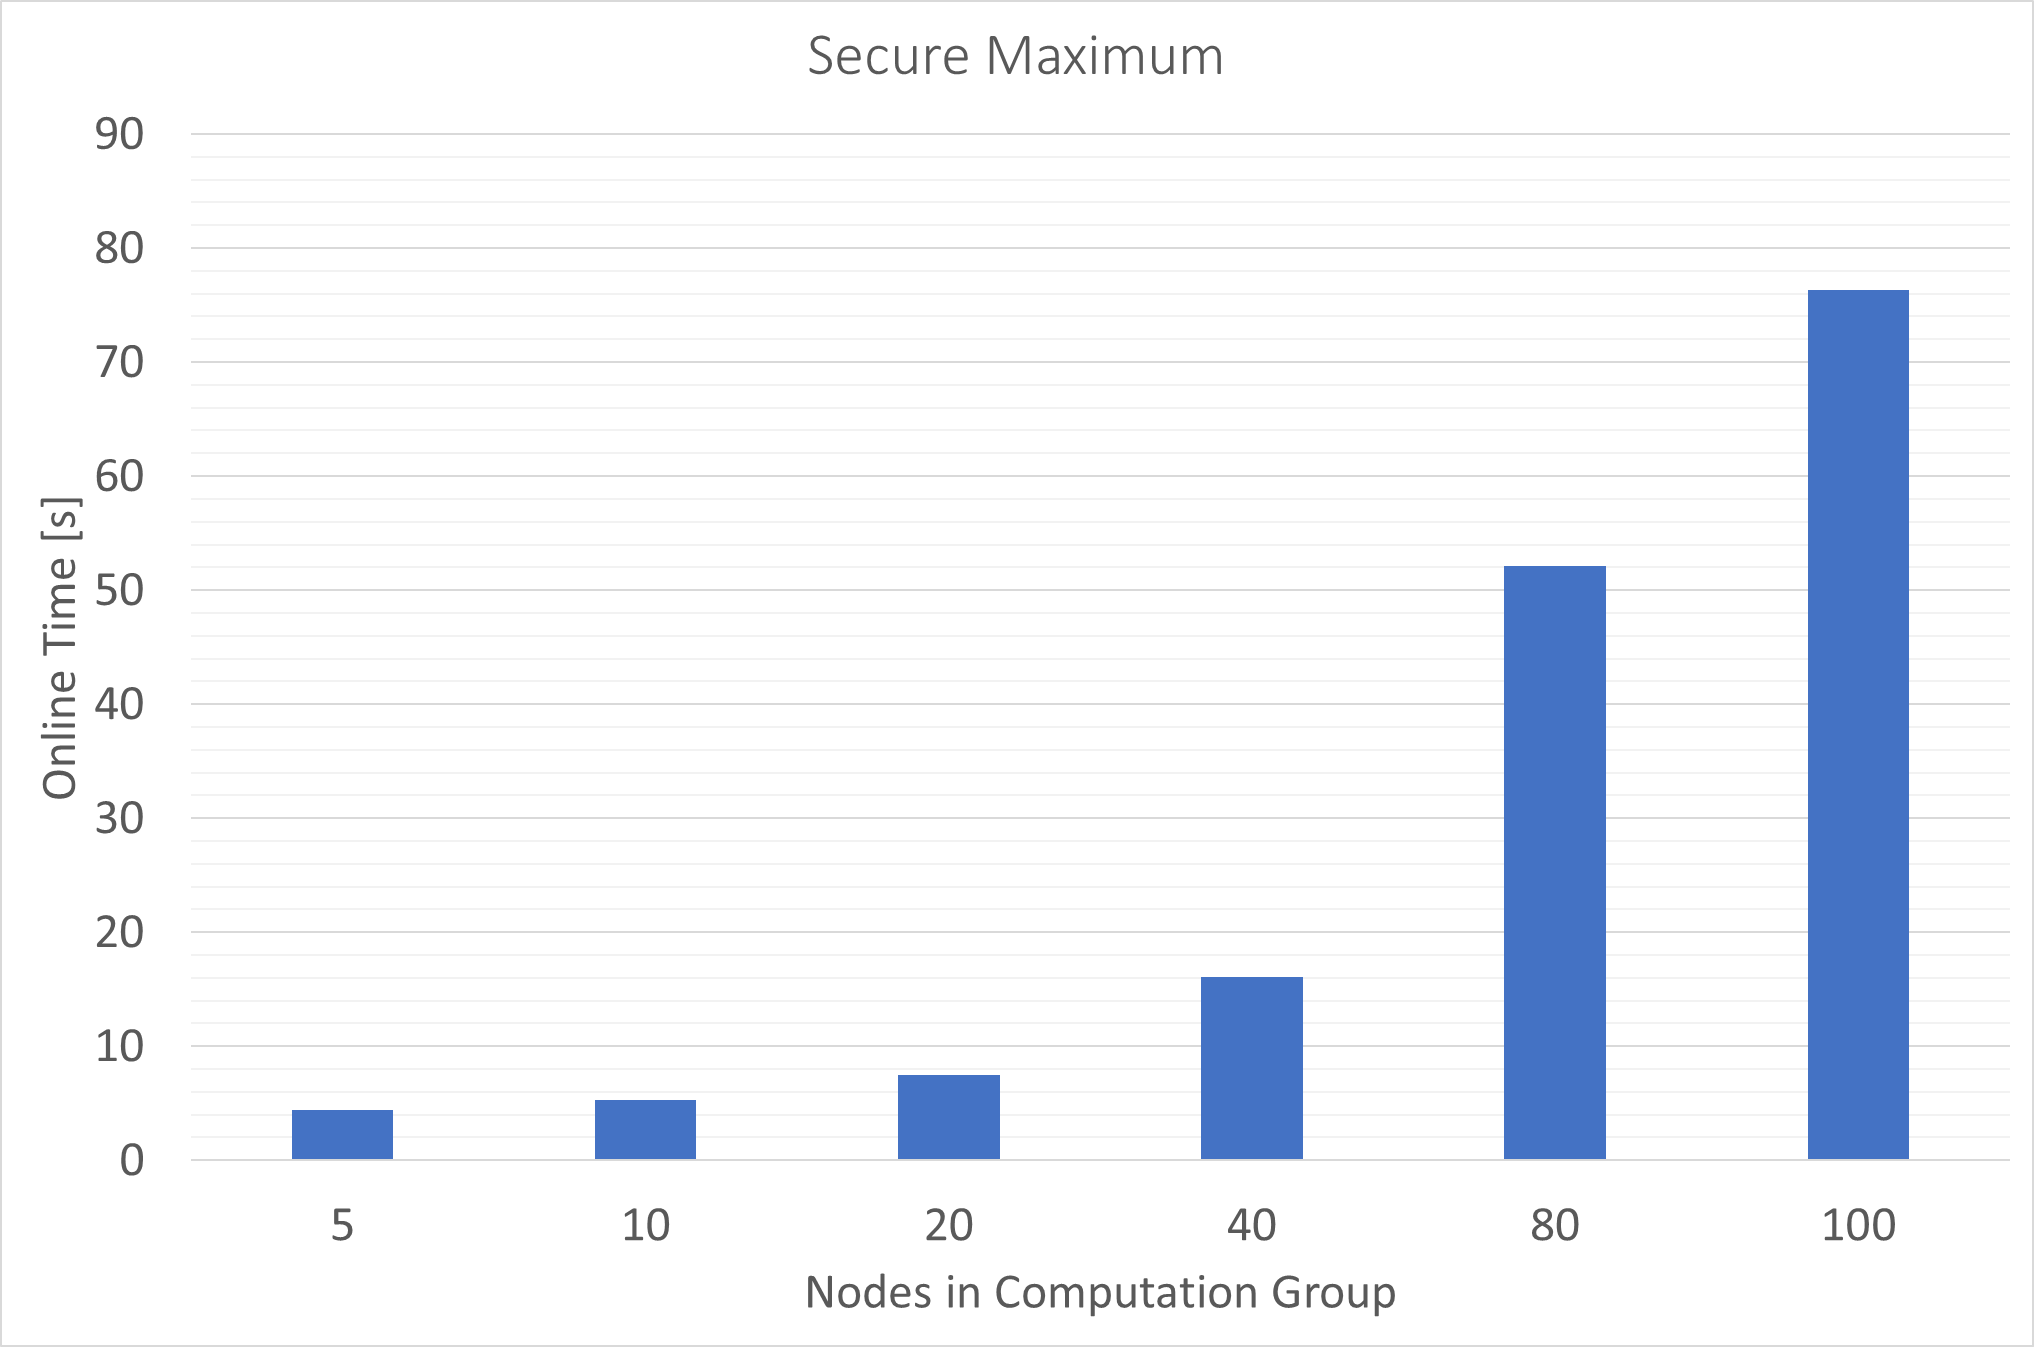
\includegraphics[scale=1.0]{figures/eval_max.png}
\end{figure}

\section{Examination of Computation Time Dependent on Computing Power} \label{Examination of Computation Time Dependent on Computing Power}
%
To evaluate the influence of computational power, the virtualization software VirtualBox was used: a Linux client running the tester application is limited through the CPU limit setting of VirtualBox. In VirtualBox the guest CPU setting can not be reduced beyond a lower bound (40\% on the development environment). Within these limits, the total computation time did not change reliable or reproducible.

As an alternative approach cpulimit\footnote{\url{https://github.com/opsengine/cpulimit}} was used to limit the cpu usage of the tester processes. Again the online time was not affected besides for very small limit-values (1 to 5\%). The measurements embedded in the code revealed however, that the usage of \lstinline|SIGSTOP| and \lstinline|SIGCONT| signals distort the measurements and the results are not reproducible.

Finally the power management of the hosting system provided reproducible results. The changes in the related computations (encryption, decryption, summation, Lagrange interpolation) are very small, therefore the fixed value for discovery was removed, to highlight the differences (see \autoref{figure:Computation time over CPU Power for 20 nodes}).

For all tests the computation group size was defined as 20. The power management was than used to limit the CPU to levels of 20\%, 40\%, 60\%, 80\% and 100\%.
\begin{figure}[!htbp] % h for placement here
	\caption{Computation time over CPU Power for 20 nodes} \label{figure:Computation time over CPU Power for 20 nodes}
	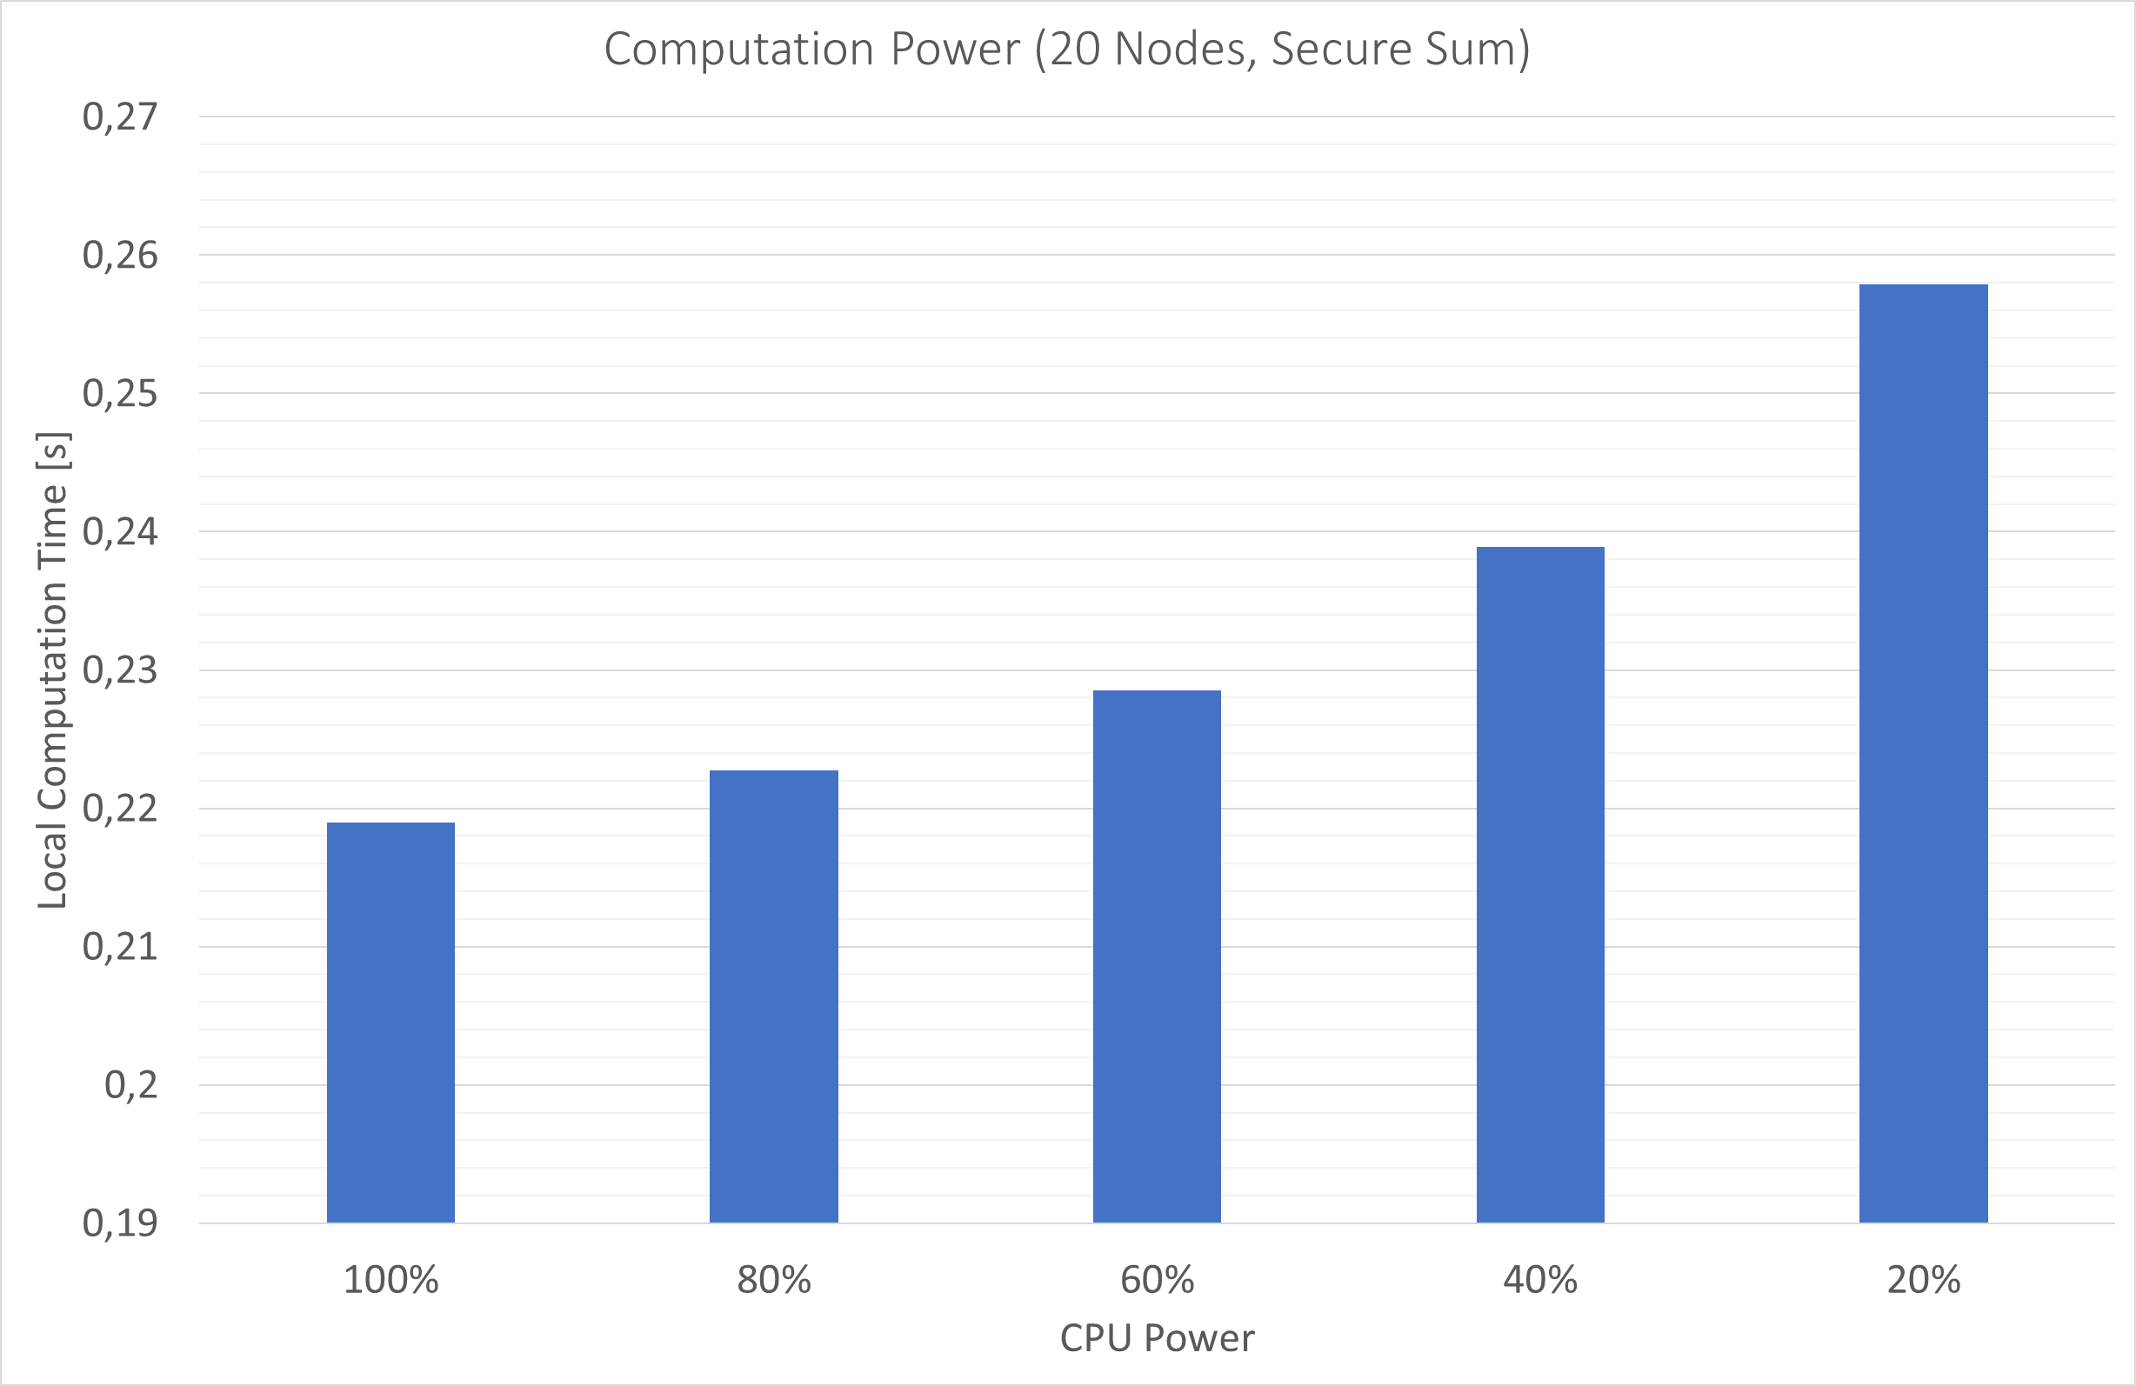
\includegraphics[scale=1.0]{figures/eval_power.png}
\end{figure}

\FloatBarrier

\chapter{Discussion} \label{Discussion}

The evaluation of the core implementation in \autoref{Evaluation} demonstrates that the framework reaches a performance grade that makes it applicable for smaller computation group sizes. Besides the computation performance, the unobtrusiveness for the end-user is also important for the successful integration of the system for example in a work environment. The demands toward the system were outlined in \autoref{Requirements} and the requirement coverage is review.
Finally solutions and improvement potential for design flaws, which were uncovered through the simulations and analysis of subroutines, are proposed for next  he evaluation also revealed first design flaws and improvement potential and solutions are proposed for the next development iterations.

\section{Requirement Satisfaction in Real-Life Settings} \label{Requirement Satisfaction in Real-Life Settings}

The usage of the framework in \glspl{MANET} with the intention to use personal smartphones as hosts, require strict compliance with the requirements regarding unobtrusiveness (\ref{req:Pairing-less Connection}), privacy protection (\ref{req:SMPC Module}) and performance (\ref{req:Performance}). In the following sections conditions for compliance are discussed in context of real-life environments.

\subsection{User Acceptance}
The results of the power consumption tests for Android (see \fullref{figure:Batterystats}) show, that having Bluetooth enabled, being discoverable and holding a \gls{RFCOMM} connection have no significance for the daily usage of a smartphone: being discoverable and connected for 24 hours consumes around the same amount of power as having the display activated for a few minutes (also analyzed through the battery stats, compare \autoref{Android battery stats report}). 
The discovery phase is expensive in regard of power consumption, but device dependent this phase is usually only active for around one to five seconds. Even for multiple retries to form a computation group, the total power consumption per hour for discovery will range significantly below 1 mA, for example if for all three \gls{SMPC} protocols 10 retries to form a computation group were needed and the device runs discovery for 5 seconds, then the power consumption for the discovery phase is $0,5$ mA in an hour. 

In regard of the power consumption the framework is therefore fit for usage and worries regarding drainage of the battery can be easily invalidated.

Further the Android tests (see \autoref{Android Bluetooth Observations}) have shown, that at least for Android devices running Android 5.0 and up, the user interaction required for joining the system is limited to the permission of becoming discoverable. Until Bluetooth is disabled, no further interactions are required and no system settings have to be manually altered. Therefore requirement \ref{req:Pairing-less Connection} is also met.

For developers \ref{req:Supportability} is met through the doxygen documentation, the clean interface provided by \lstinline|node.h| and the implementations in the tester application and the Android example. For \ref{req:Usability} all settings are adjusted in \lstinline|configurations.h|, simplifying the framework adaption and integration. 
As described in \autoref{Interfacing the Library}, \ref{req:Expandability} is not fully met yet. The \gls{MAC} address bound identification of devices will be further abstracted to decouple the framework from a specific wireless technology.

\subsection{Required Time for Computation}

Since the system is intended for a \gls{MANET}, the computation time has to stay within limits, so that the computation can complete before the fully meshed computation group network is separated.

In the secure sum protocol for lower node numbers, the discovery is the major time consumer and up to 20 nodes, the computational costs are comparatively negligible. For larger computation groups, the time needed to compute the secure sum reaches durations that make a network separation for moving nodes likely. Bluetooth range varies significantly among Bluetooth modules and power settings, but a range of 10 meters is a good rule of thumb. Considering a typical walking speed of 1,4 meters per second \autocite{Mohler2007}, the distance after 7 seconds (compare \autoref{figure:walking range in computation time}) makes it likely that the connection to other nodes is lost because of the distance or shielding walls, especially if the other nodes are moving as well.

\begin{figure}[!htbp] % h for placement here
	\caption{Walking range in computation time} \label{figure:walking range in computation time}
	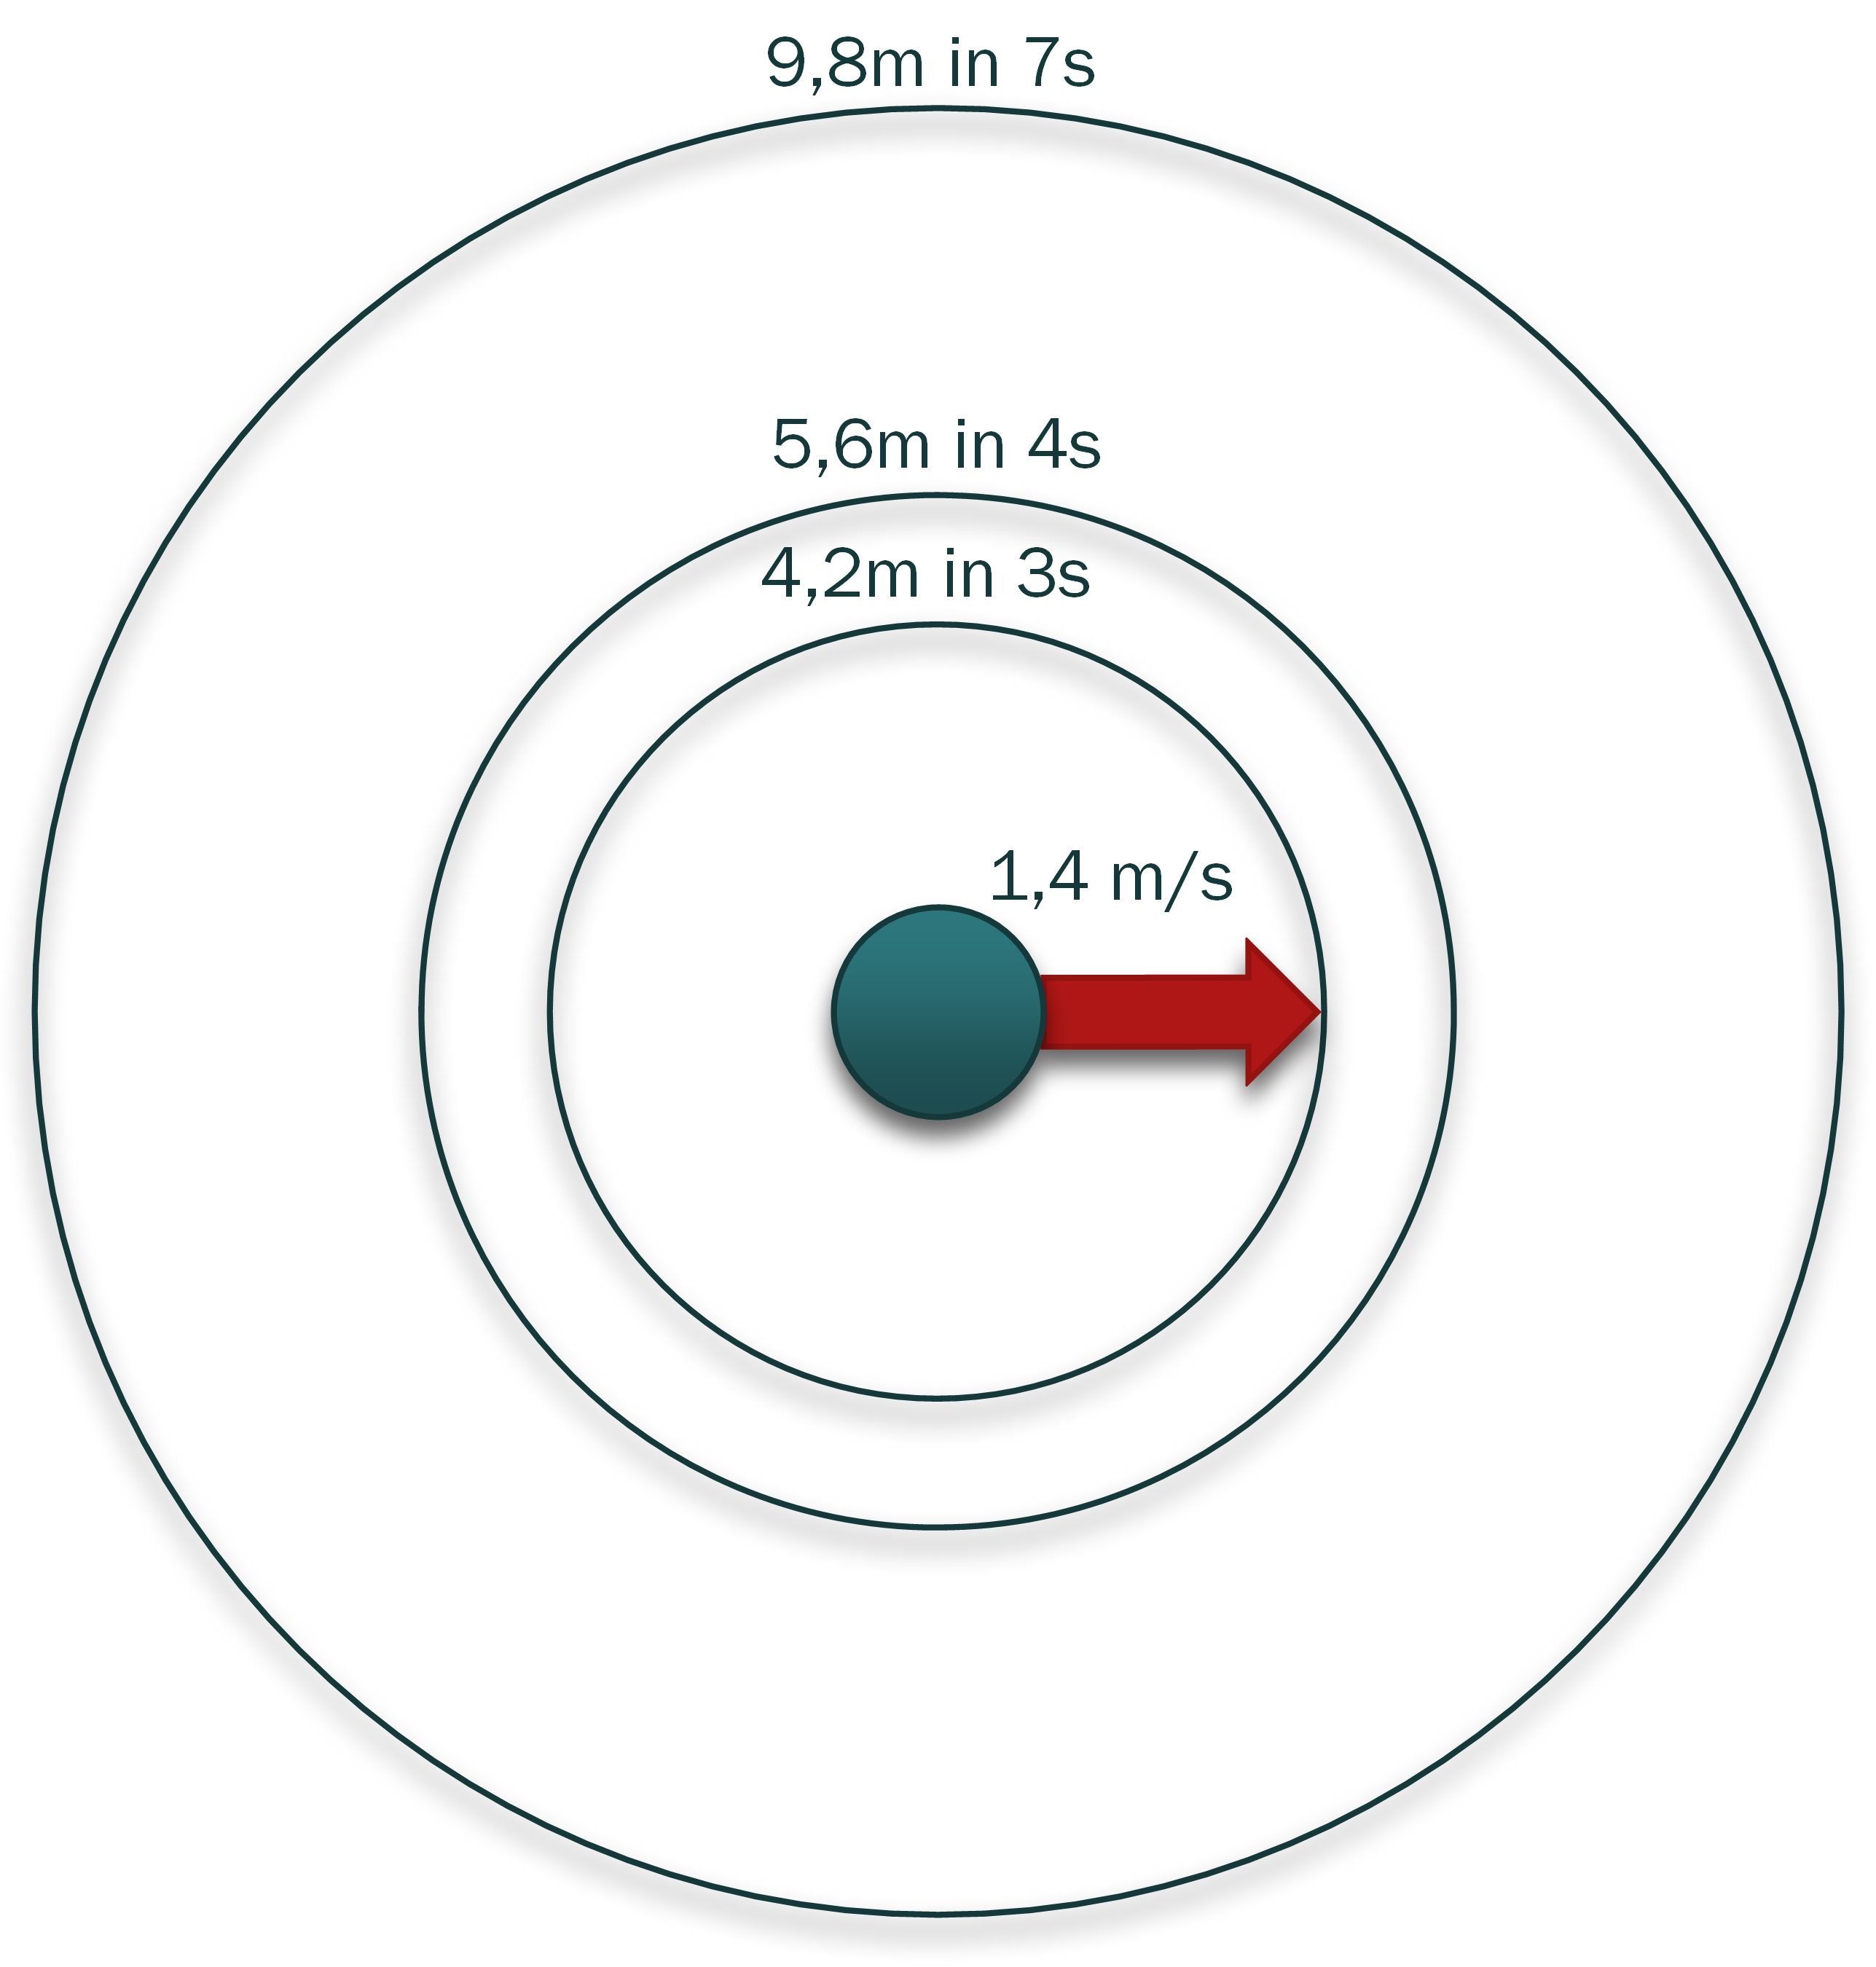
\includegraphics[scale=1.0]{figures/walking_range.png}
\end{figure}

The core implementation provided in \autoref{Implementation} meets requirements \ref{req:Coordinator Election}, \ref{req:Token-Passing} and \ref{req:SMPC Module}, though based on the current performance simulations of the system (see \autoref{figure:Computation time over number of nodes for secure sum} and \autoref{figure:Computation time over number of nodes for secure maximum}) \ref{req:Performance} is only met for small computation groups ($n<20$). Since the simulations in \autoref{Evaluation} do not take into account durations needed for establishing the \gls{RFCOMM} connections, the simulations need to be adjusted based on further measurements on different Android devices. The development goal for the tester application is to make it a tool for analyzing the performance of the framework in the intended system configuration.

The tests regarding computational power have shown, that the reduction of the online phase through scale up of the nodes is limited: the message driven nature of the system and the high amount of massages (raising with the number of nodes squared) passed between the nodes in a sequential manner are not transmitted faster when upscaling. This demonstrates that the framework can tolerate nodes with comparatively low computational power, but the influence of the messages also request optimization of the message system (see \autoref{Design Flaws Detected Through Evaluation}).

\section{Design Flaws Discussion} \label{Design Flaws Detected Through Evaluation}

Since the sequential message passing between the nodes is causing a significant computation delay, the design needs to be optimized. The message format holds potential for optimization as well as the message exchange protocol.
Message format improvements:
\begin{itemize}
	\item Currently the messages are zero terminated strings, which simplified the first implementation, but it also generates overhead: each message holds the additional termination character and numbers are digit-wise converted into ASCII characters. For a signed integer of eleven digit length, this produces an overhead of 8 bytes. Therefore all messages with known payload size can be transmitted in the native data type to reduce overhead. For encrypted messages this provides no message reduction though, because short messages are padded to the block size (16 byte).
	\item The \gls{MAC} addresses are transmitted as passed from the host in the colon-separated form. Removing the separating colons removes 5 byte per \gls{MAC} address.
	\item The \lstinline|Broadcast_Request| enumerator can be defined as the upper bound for all message types.  Instead of concatenating the broadcast and the message request, the sum of booth can be used as message type. Using $127$ as the broadcast value leaves $0$ to $126$ as message type values, while keeping the sum within a byte's length. The receiving node checks if the message type is larger than the broadcast request value to identify a broadcast request. This reduces the broadcast requests by 3 bytes.
\end{itemize}

Similar to software parallelization, where load is distributed among threads, in some cases the sequential message passing can be distributed among nodes:
\begin{itemize}
	\item Instead of sending each node in the computation group sequentially a broadcast message (compare \autoref{figure:Broadcast optimization - a}), the coordinator can distribute broadcasts with large payloads among nodes, which in turn transmit the message to a subgroup of nodes. The coordinator then sends \lstinline|ACK|-requests to each node to verify all nodes are ready (see \autoref{figure:Broadcast optimization - b}).
\end{itemize}

\begin{figure}[!htb] % h for placement here
	\centering
	\subfloat[Current implementation of computation group announcement]{%
		\label{figure:Broadcast optimization - a}
		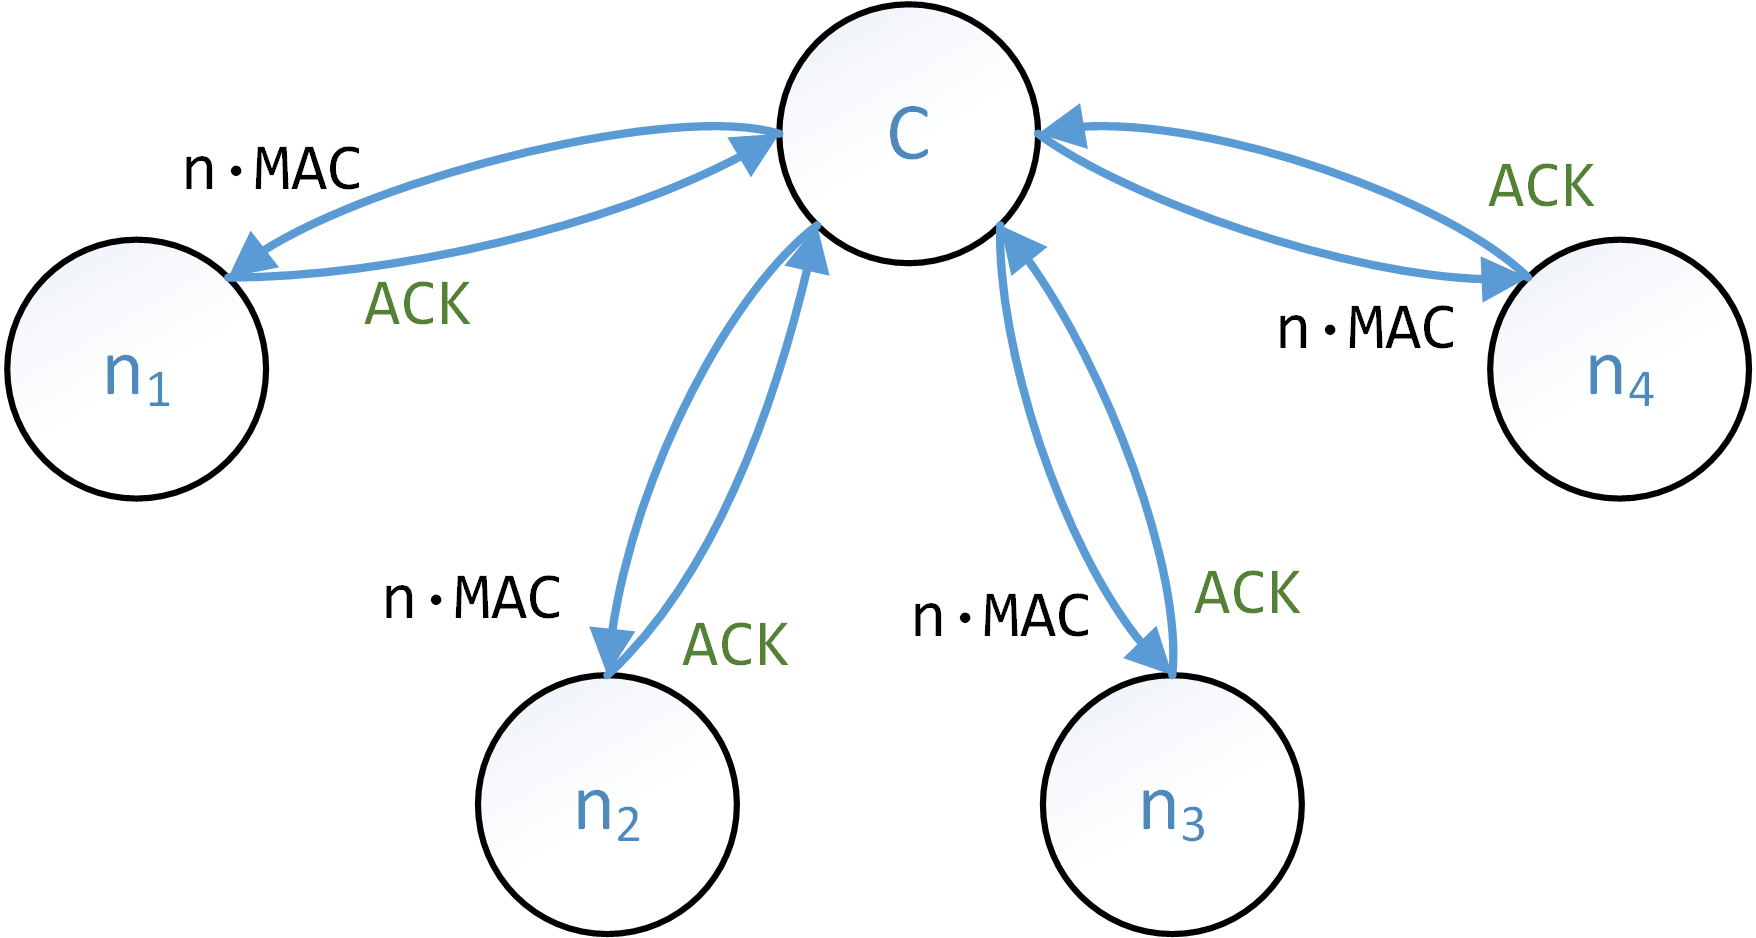
\includegraphics[scale=1.0]{figures/broadcast_distribution_old.png}
		
	}\\
	\subfloat[Improved computation group announcement]{%
		\label{figure:Broadcast optimization - b}
		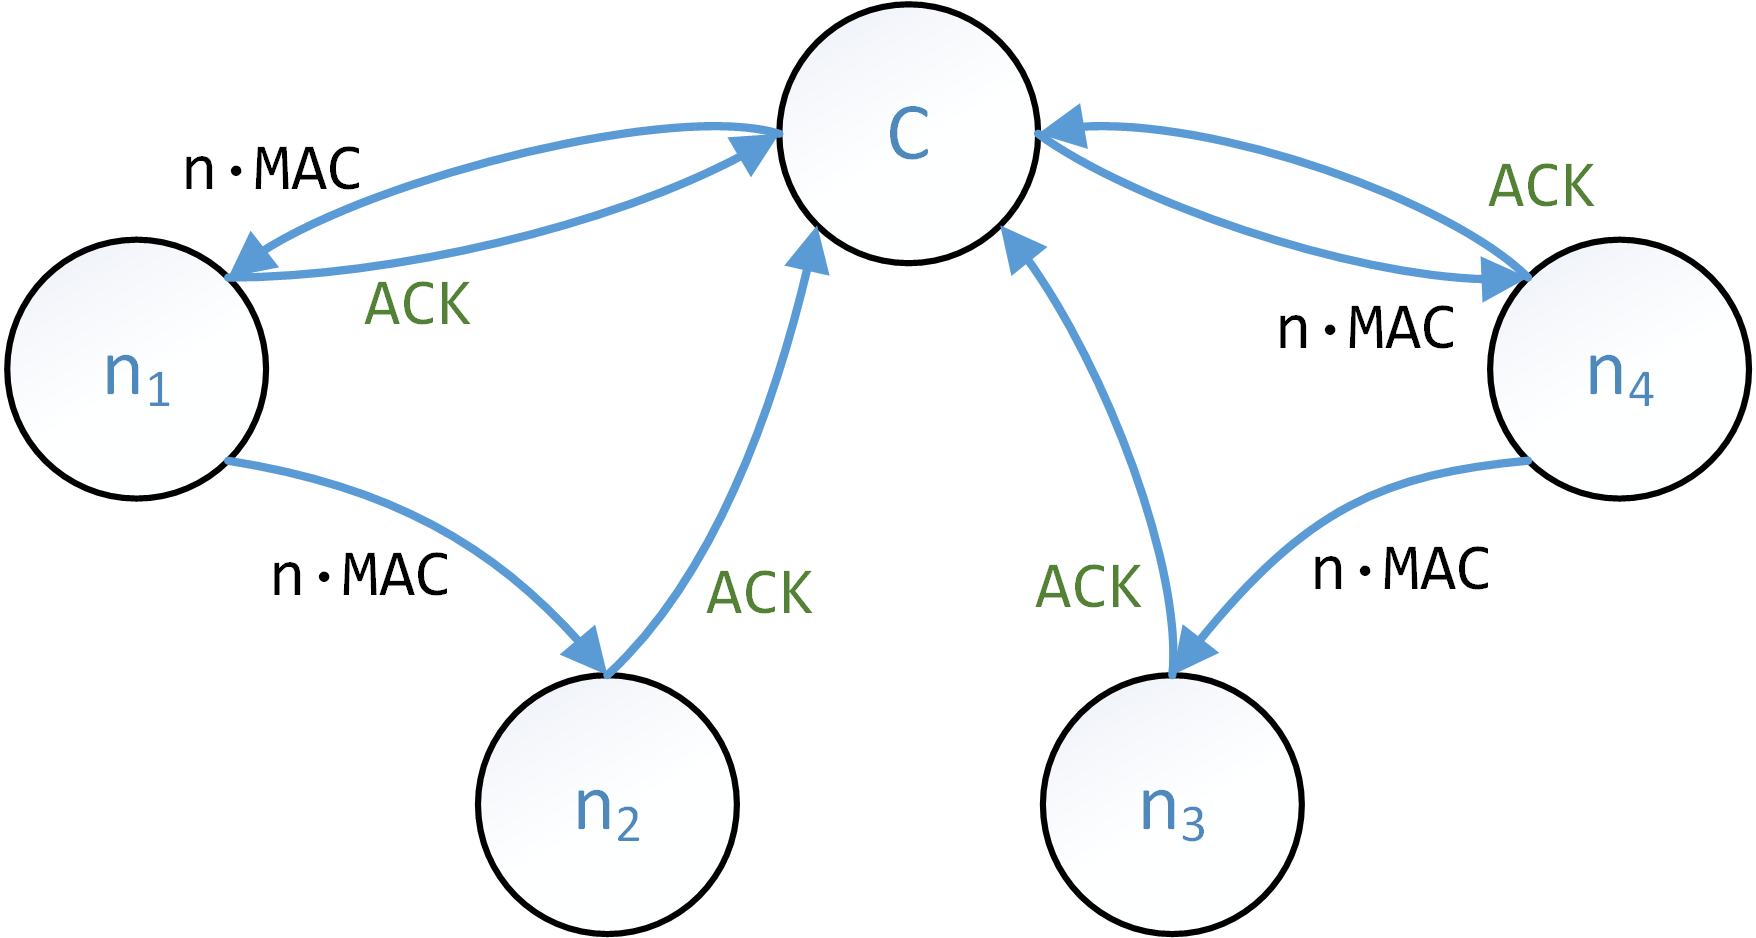
\includegraphics[scale=1.0]{figures/broadcast_distribution_new.png}
	}
	\caption{Broadcast optimization} \label{figure:broadcast optimization}
\end{figure}
 
Protocol improvements:
\begin{itemize}
	\item The sum protocol currently limits the computation group, because an 32 bit integer is computed and returned. For larger scores, this can cause a integer overflow if the computation group is lager than the maximum value of the data type divided by the maximum score. Because of the expected group sizes based on \autoref{Evaluation}, using a 64 bit integer will fix the overflow risk.
	\item A fixed size computation group reduces the online-phase and is therefore the preferred setting, but this will leave single nodes without the option to commit their scores. The computation priority should increase for these node. When a threshold is reached, the computation can tolerate a number of nodes (similar to the threshold for adversaries) using computation results as inputs. This has to be evaluated for correctness and privacy.
\end{itemize}

For the real-life usage a quality of service feature will be useful: if the configurations of the framework provide a high grade of privacy (larger computation group) but cause many network separation while computing, the user should be informed. For the assessment the following events should be collected:
\begin{enumerate}
	\item Forming of computation group was unsuccessful.
	\item Computation was aborted due to network separation.
\end{enumerate}

Using these values as a metric for system performance, the maintainer can then change the computation group size to improve the chances for computation completion.

%Based on the gamification related target group, assumptions regarding the significance of dated data can be made: for example it is of interest to compare the general average for the previous year with the personal scores, maybe also on month or week level. In contrast a more fine-grained resolution of dated data will be rarely used while requiring extensive storage, compared to summarized data.

\FloatBarrier

\chapter{Conclusion} \label{Conclusion}

\todo*{5-10\%; outcome for an introduction-reader}

\todo*{describe how statements in the introduction were met: \gls{SMPC} over self-forming, low maintenance/infrastructure-less network; framework offers reduced complexity, useful computation results for many gamification settings and other applications; performance for real life usage with good levels of security; outlook: will gain more significance for SIoT: secure Internet of things (revisit topic of insecure Internet); next steps: host public as open source to gain to use open source community to improve project further}

\clearpage
\renewcommand{\bibname}{References} % rename Bibliograpy to References

\begingroup
\sloppy
\printbibliography[heading=bibintoc] % add References chapter and display it in toc
\endgroup



%\begin{appendices}
%	\chapter{Some name}
%	\lipsum[3]
%\end{appendices}

%\todos

\end{document}